%!TEX root = ../dissertation.tex
\begin{savequote}[75mm]
Age wears the flesh but galvanizes the soul.   
\end{savequote}
\chapter{Effects from variations in the sideband and control region definitions}
\label{app:appendixSysVar}

\paragraph{}
This Appendix is the supporting material for section~\ref{sec:non-closure-mu-qcd}. 
The effect on signal region yield from different control region and sideband region definitions is tested. 
All these tests are done on the control/sideband regions after the full reweighting procedure as described in \ref{sec:boosted-reweight} while applying the nominal reweighting values.

\paragraph{}
In addition to the nominal control region and sideband region definitions, seven additional variations, as illustrated in Figures~\ref{CRSB:CR_High}, \ref{CRSB:CR_Low}, \ref{CRSB:CR_Small}, \ref{CRSB:SB_High}, \ref{CRSB:SB_Low}, \ref{CRSB:SB_Large}, \ref{CRSB:SB_Small}. 
They are defined in section~\ref{sec:non-closure-mu-qcd}.

\paragraph{}
The high mass and low mass CR test how background modeling is sensitive to the exact position of CR. 
The signal-depletion CR is designed to test whether there is significant signal contamination in the CR. 
If there is a large amount of signal contamination in CR, the agreement between data and prediction in the CR would be significantly different from the number calculated with nominal CR. 
The sideband variations are designed to test how sensitive the normalization fit is to the sideband definition.

\paragraph{}
The agreement between data and prediction in CR are summarized in Tables~\ref{tab:Tab_4b_CR_Variations}, \ref{tab:Tab_3b_CR_Variations}, and \ref{tab:Tab_2bs_CR_Variations}.
For most CR variations, the discrepancy between data and prediction is smaller than the statistical uncertainty of data. 
The only exception is $2bs$ high CR variation, where the prediction is $\sim 1.5 \sigma$ away from the data.
The signal-depletion CR definition shows no significant deviation in yield from the nominal CR definition.
The discrepancy is within the statistical uncertainty of data as well.
This shows that no significant signal contamination in the CR is found.

\begin{figure}[htbp!]
\centering
\captionsetup{justification=centering}
    \begin{subfigure}[b]{0.39\textwidth}
        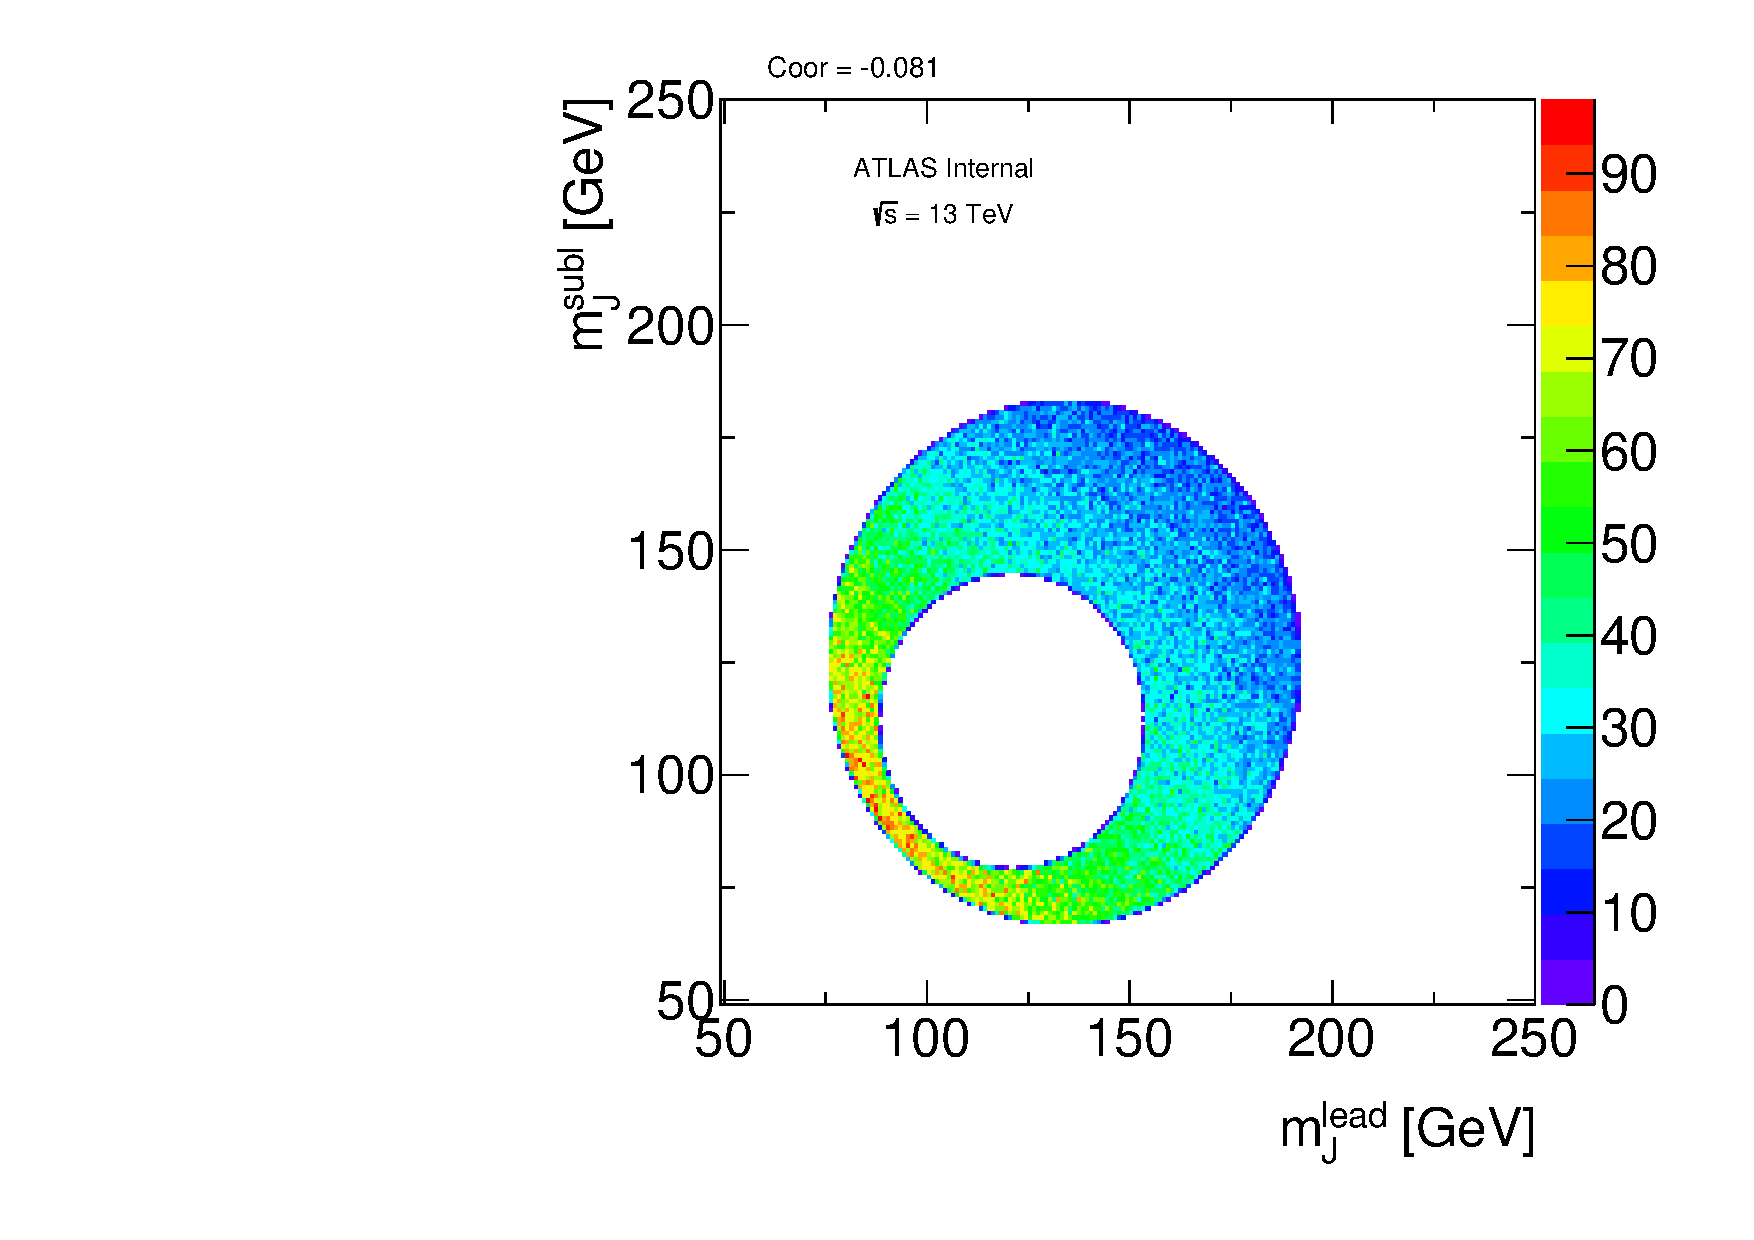
\includegraphics[width=\textwidth,angle=-90]{figures/boosted/Syst_CRSB/CR_Low_Sideband_OneTag_mH0H1.pdf}
        \caption{Sideband region}
        \label{CRSB:CR_Low_SB}
    \end{subfigure}
    \quad
    \begin{subfigure}[b]{0.39\textwidth}
        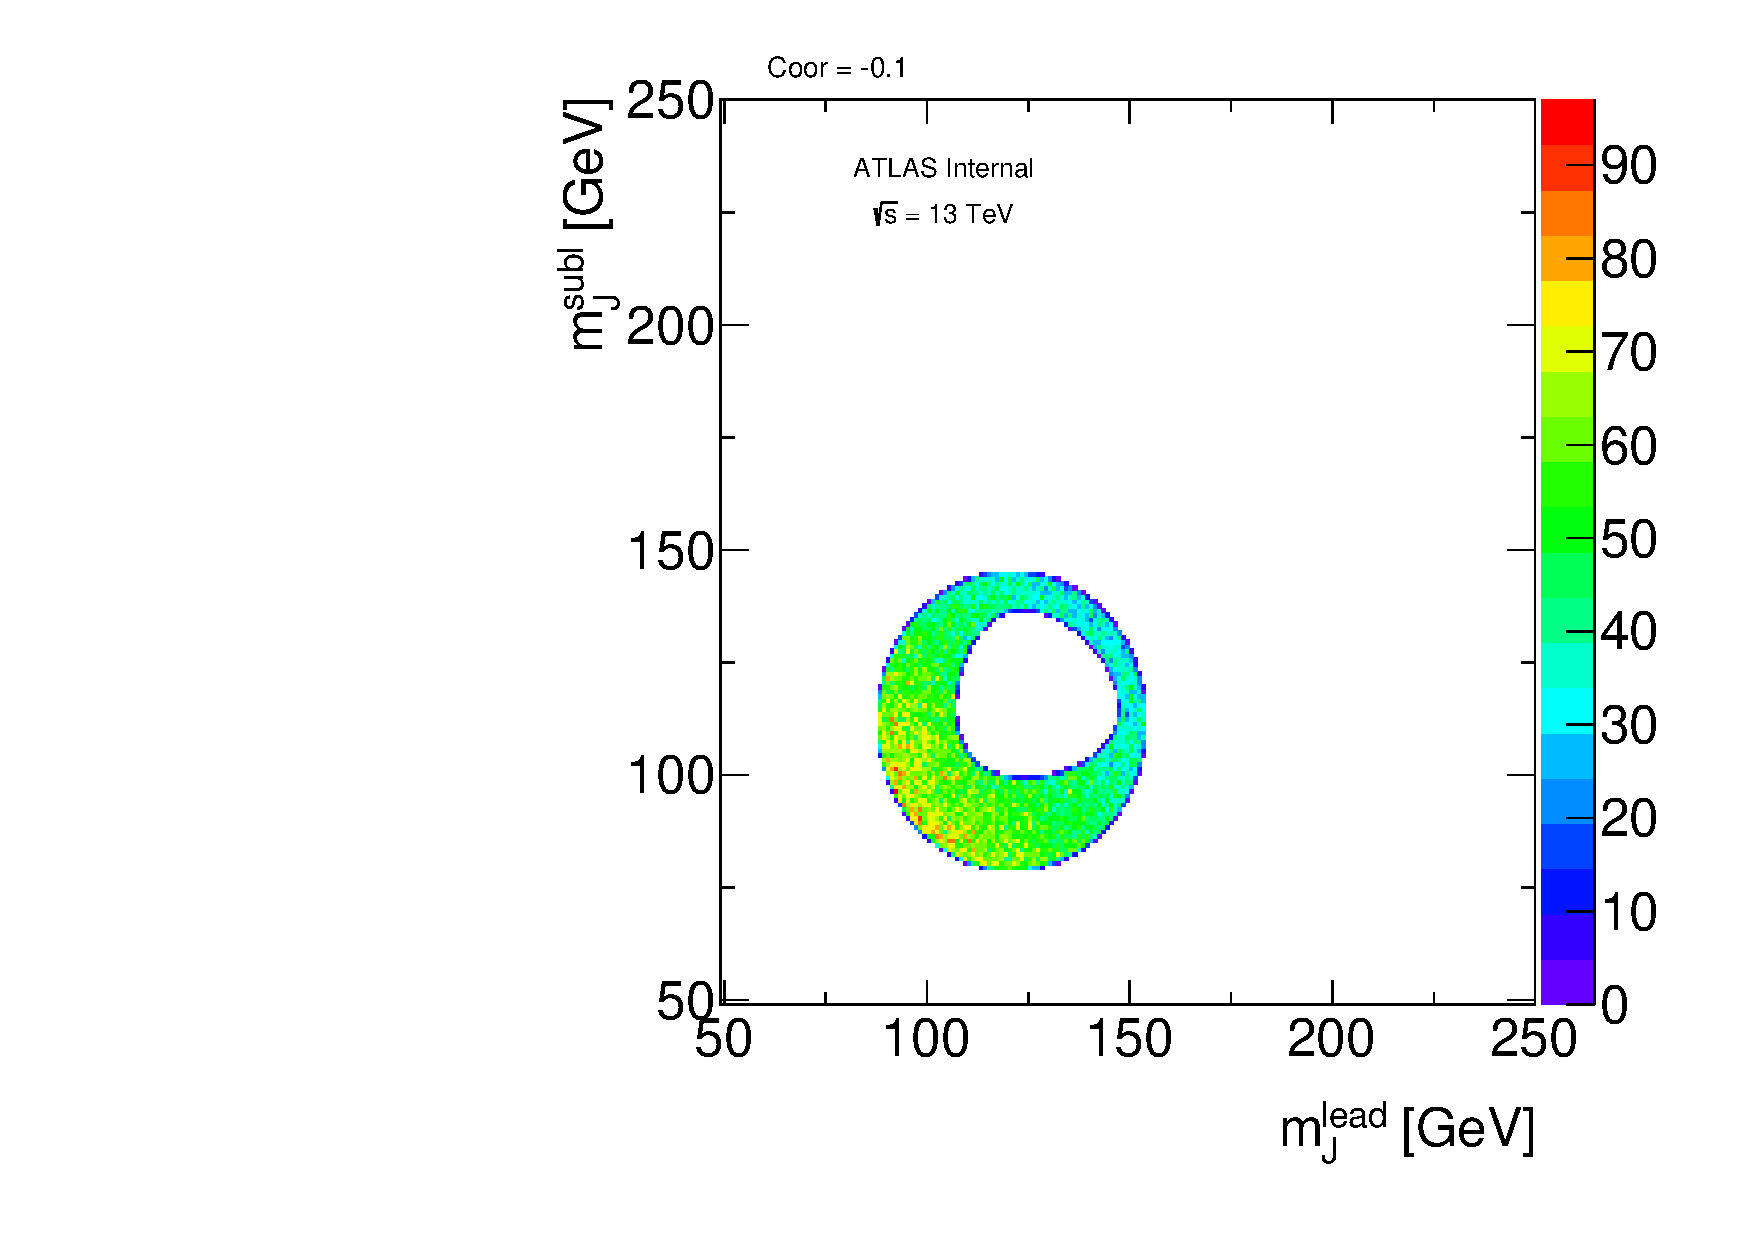
\includegraphics[width=\textwidth,angle=-90]{figures/boosted/Syst_CRSB/CR_Low_Control_OneTag_mH0H1.pdf}
        \caption{Control region}
        \label{CRSB:CR_Low_CR}
    \end{subfigure}
\caption{In $1b$ data, with the low-mass CR variation, new SB and CR \mleadJ-\msublJ~ distributions.}
\label{CRSB:CR_Low}
\end{figure}


\begin{figure}[htbp!]
\centering
\captionsetup{justification=centering}
    \begin{subfigure}[b]{0.39\textwidth}
        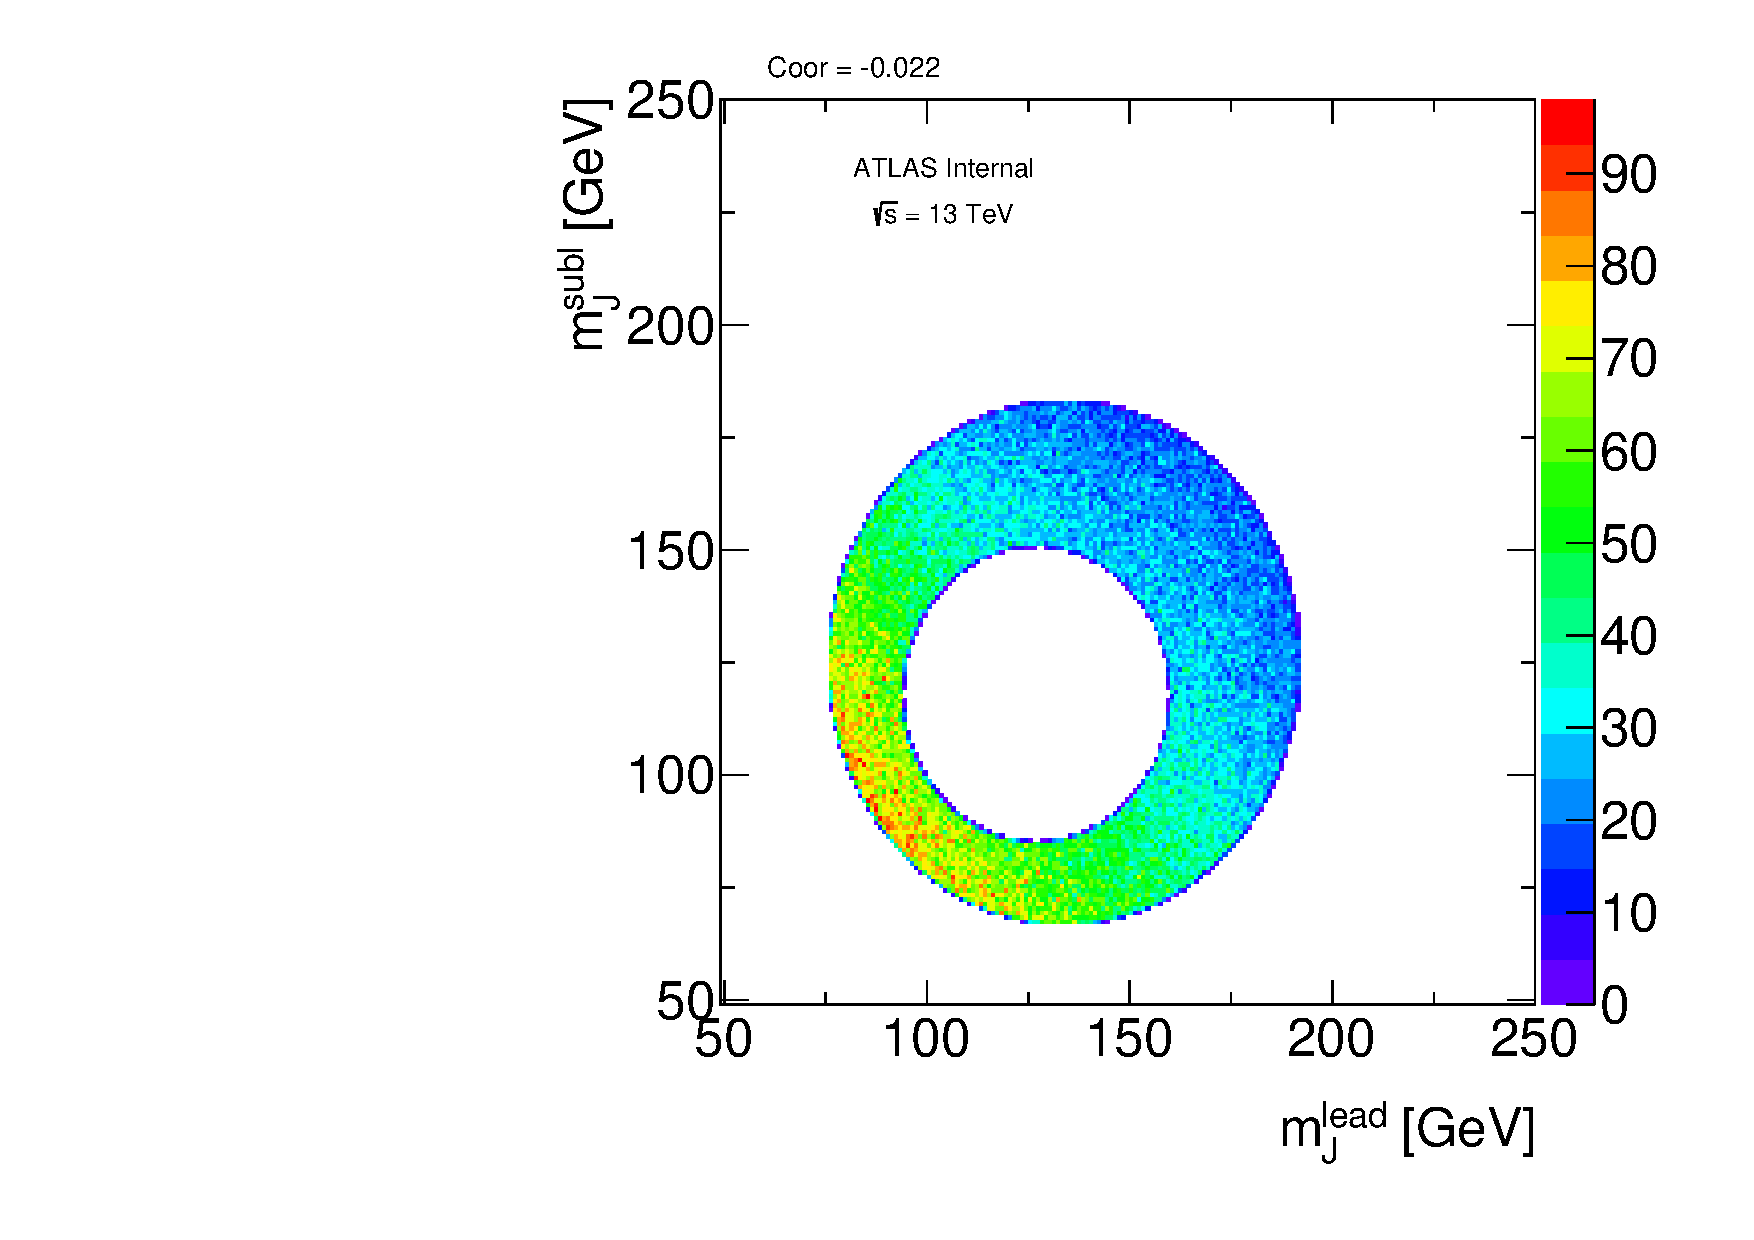
\includegraphics[width=\textwidth,angle=-90]{figures/boosted/Syst_CRSB/CR_High_Sideband_OneTag_mH0H1.pdf}
        \caption{Sideband region}
        \label{CRSB:CR_High_SB}
    \end{subfigure}
    \quad
    \begin{subfigure}[b]{0.39\textwidth}
        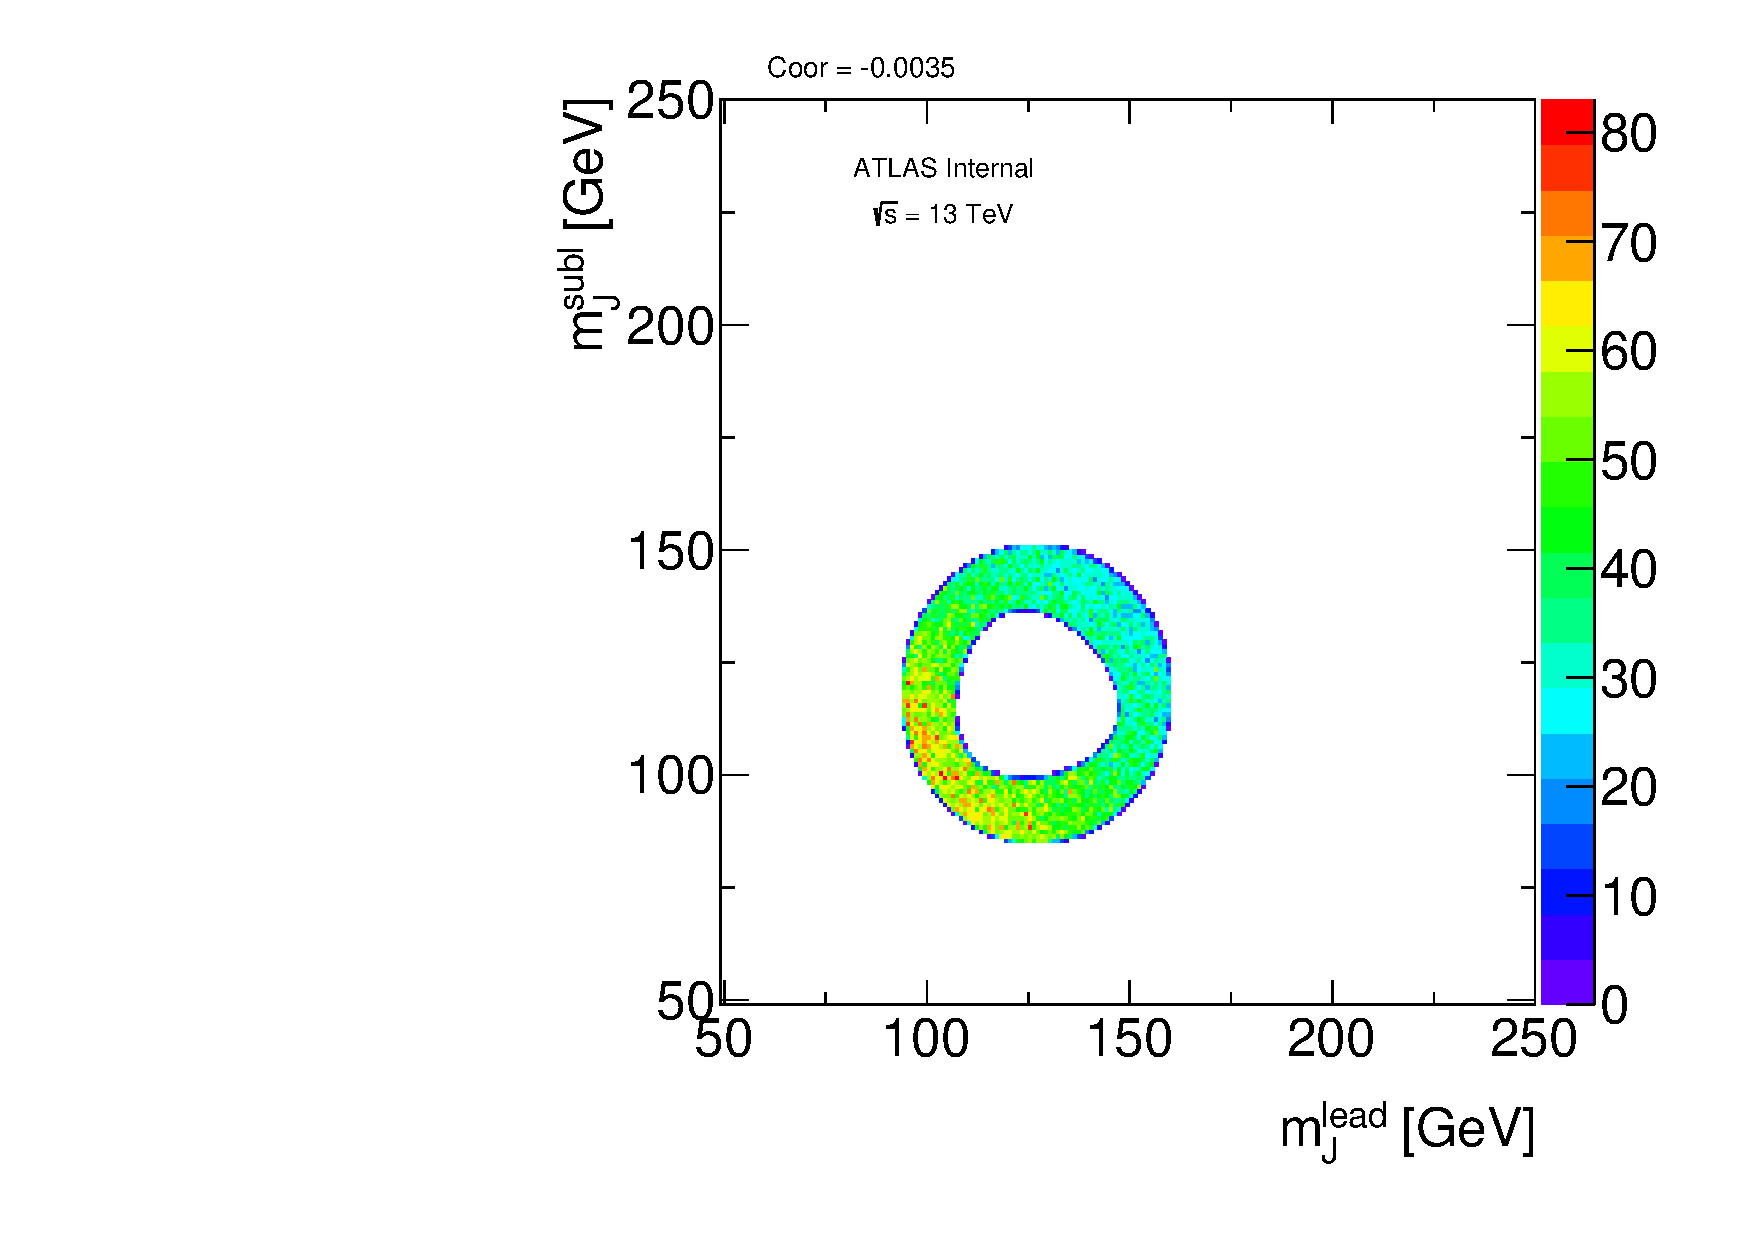
\includegraphics[width=\textwidth,angle=-90]{figures/boosted/Syst_CRSB/CR_High_Control_OneTag_mH0H1.pdf}
        \caption{Control region}
        \label{CRSB:CR_High_CR}
    \end{subfigure}
\caption{In $1b$ data, with the high-mass CR variation, new SB and CR \mleadJ-\msublJ~ distributions.}
\label{CRSB:CR_High}
\end{figure}

\begin{figure}[htbp!]
\centering
\captionsetup{justification=centering}
    \begin{subfigure}[b]{0.39\textwidth}
        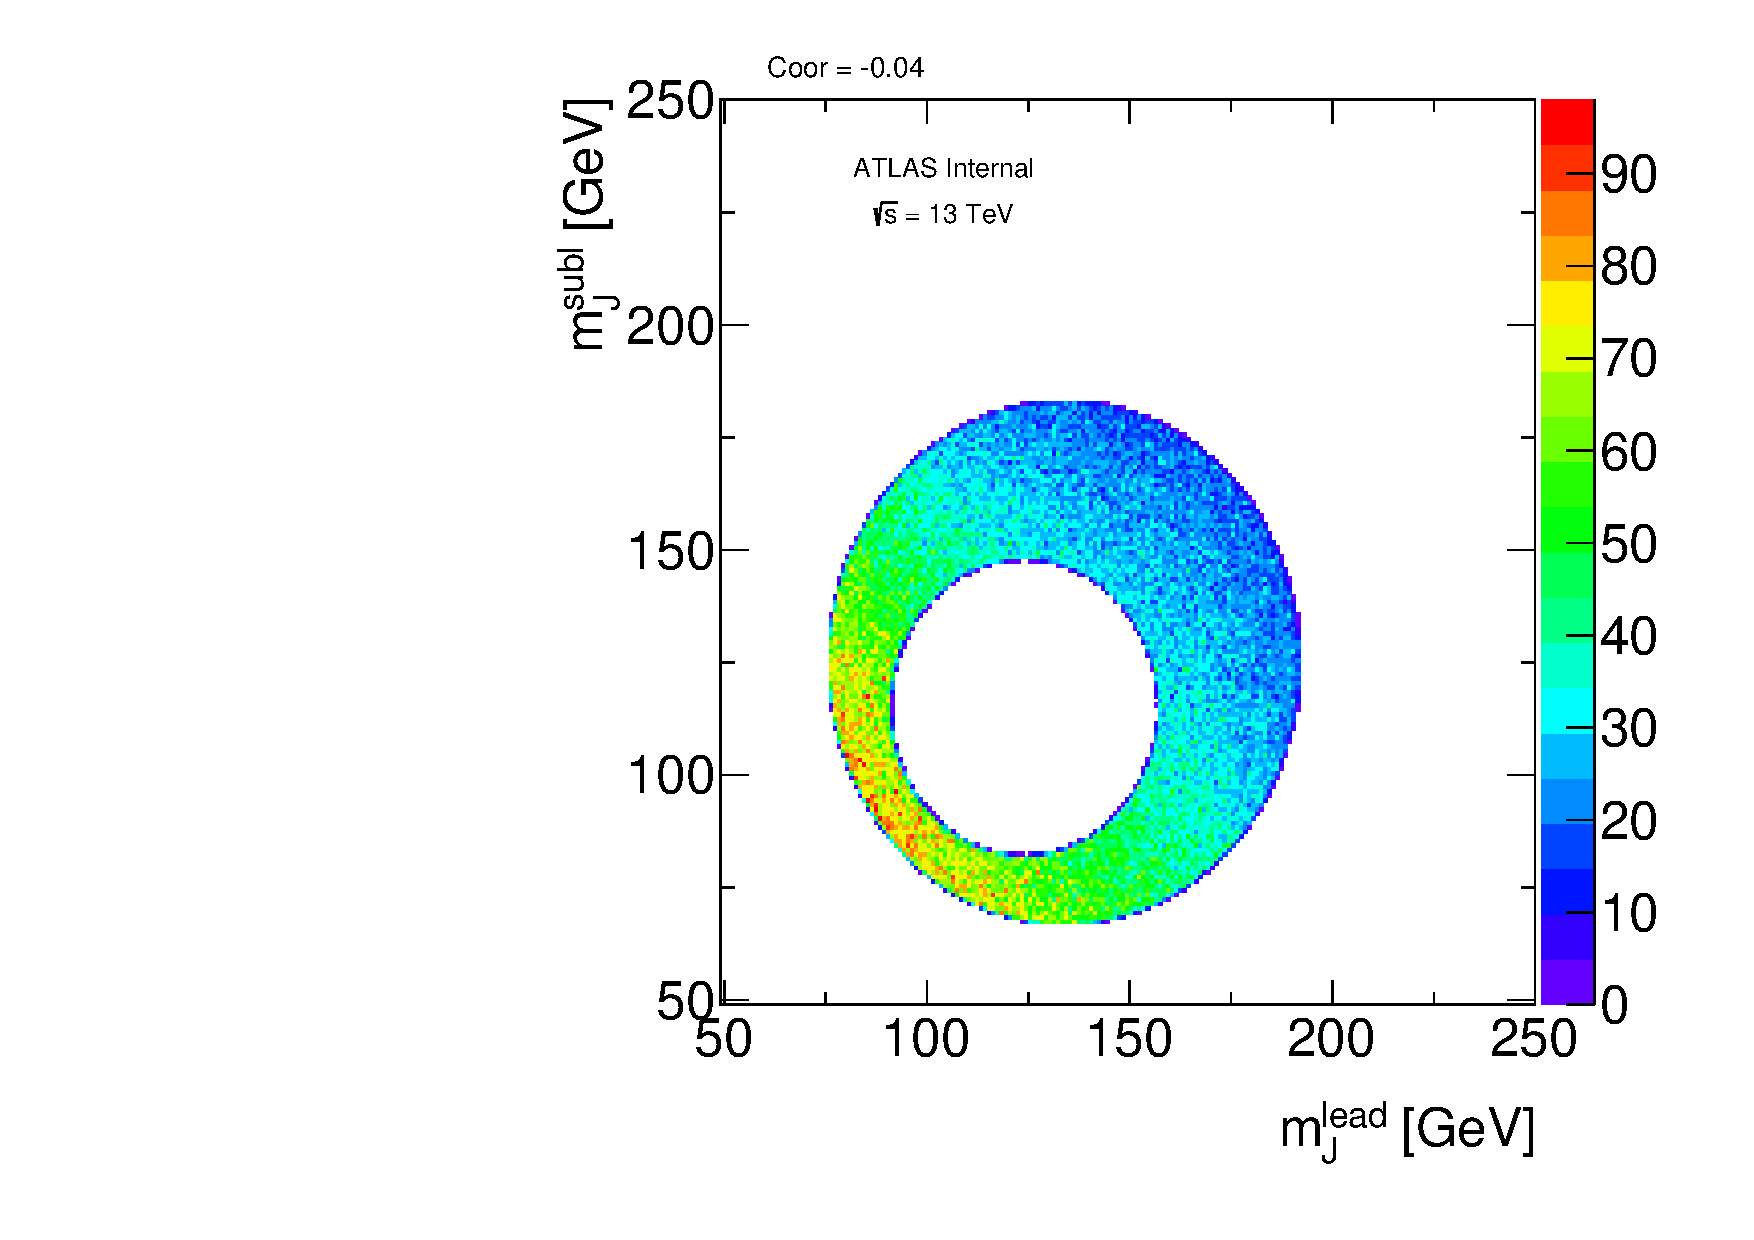
\includegraphics[width=\textwidth,angle=-90]{figures/boosted/Syst_CRSB/CR_Small_Sideband_OneTag_mH0H1.pdf}
        \caption{Sideband region}
        \label{CRSB:CR_Small_SB}
    \end{subfigure}
    \quad
    \begin{subfigure}[b]{0.39\textwidth}
        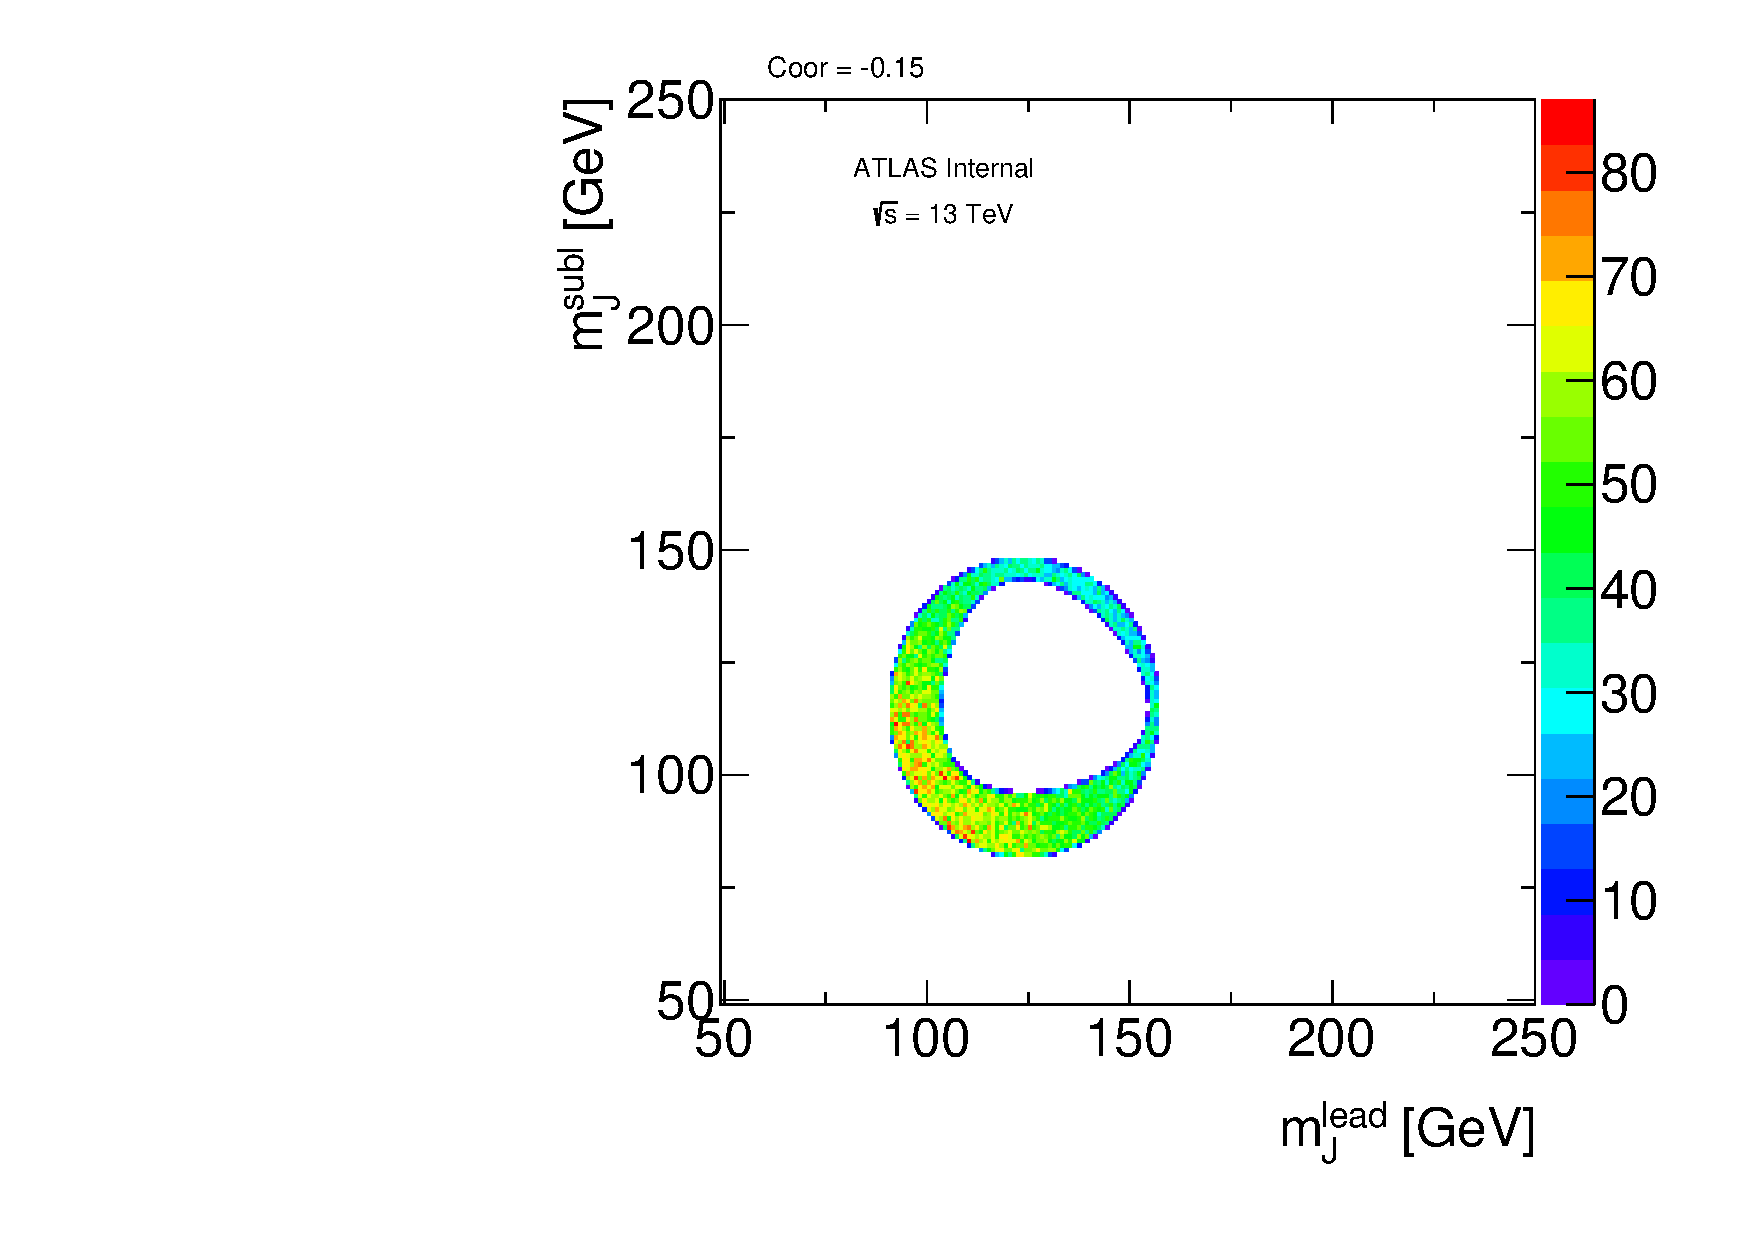
\includegraphics[width=\textwidth,angle=-90]{figures/boosted/Syst_CRSB/CR_Small_Control_OneTag_mH0H1.pdf}
        \caption{Control region}
        \label{CRSB:CR_Small_CR}
    \end{subfigure}
\caption{In $1b$ data, with the signal-depletion (small) CR variation, new SB and CR \mleadJ-\msublJ~ distributions.}
\label{CRSB:CR_Small}
\end{figure}

\begin{figure}[htbp!]
\centering
\captionsetup{justification=centering}
    \begin{subfigure}[b]{0.39\textwidth}
        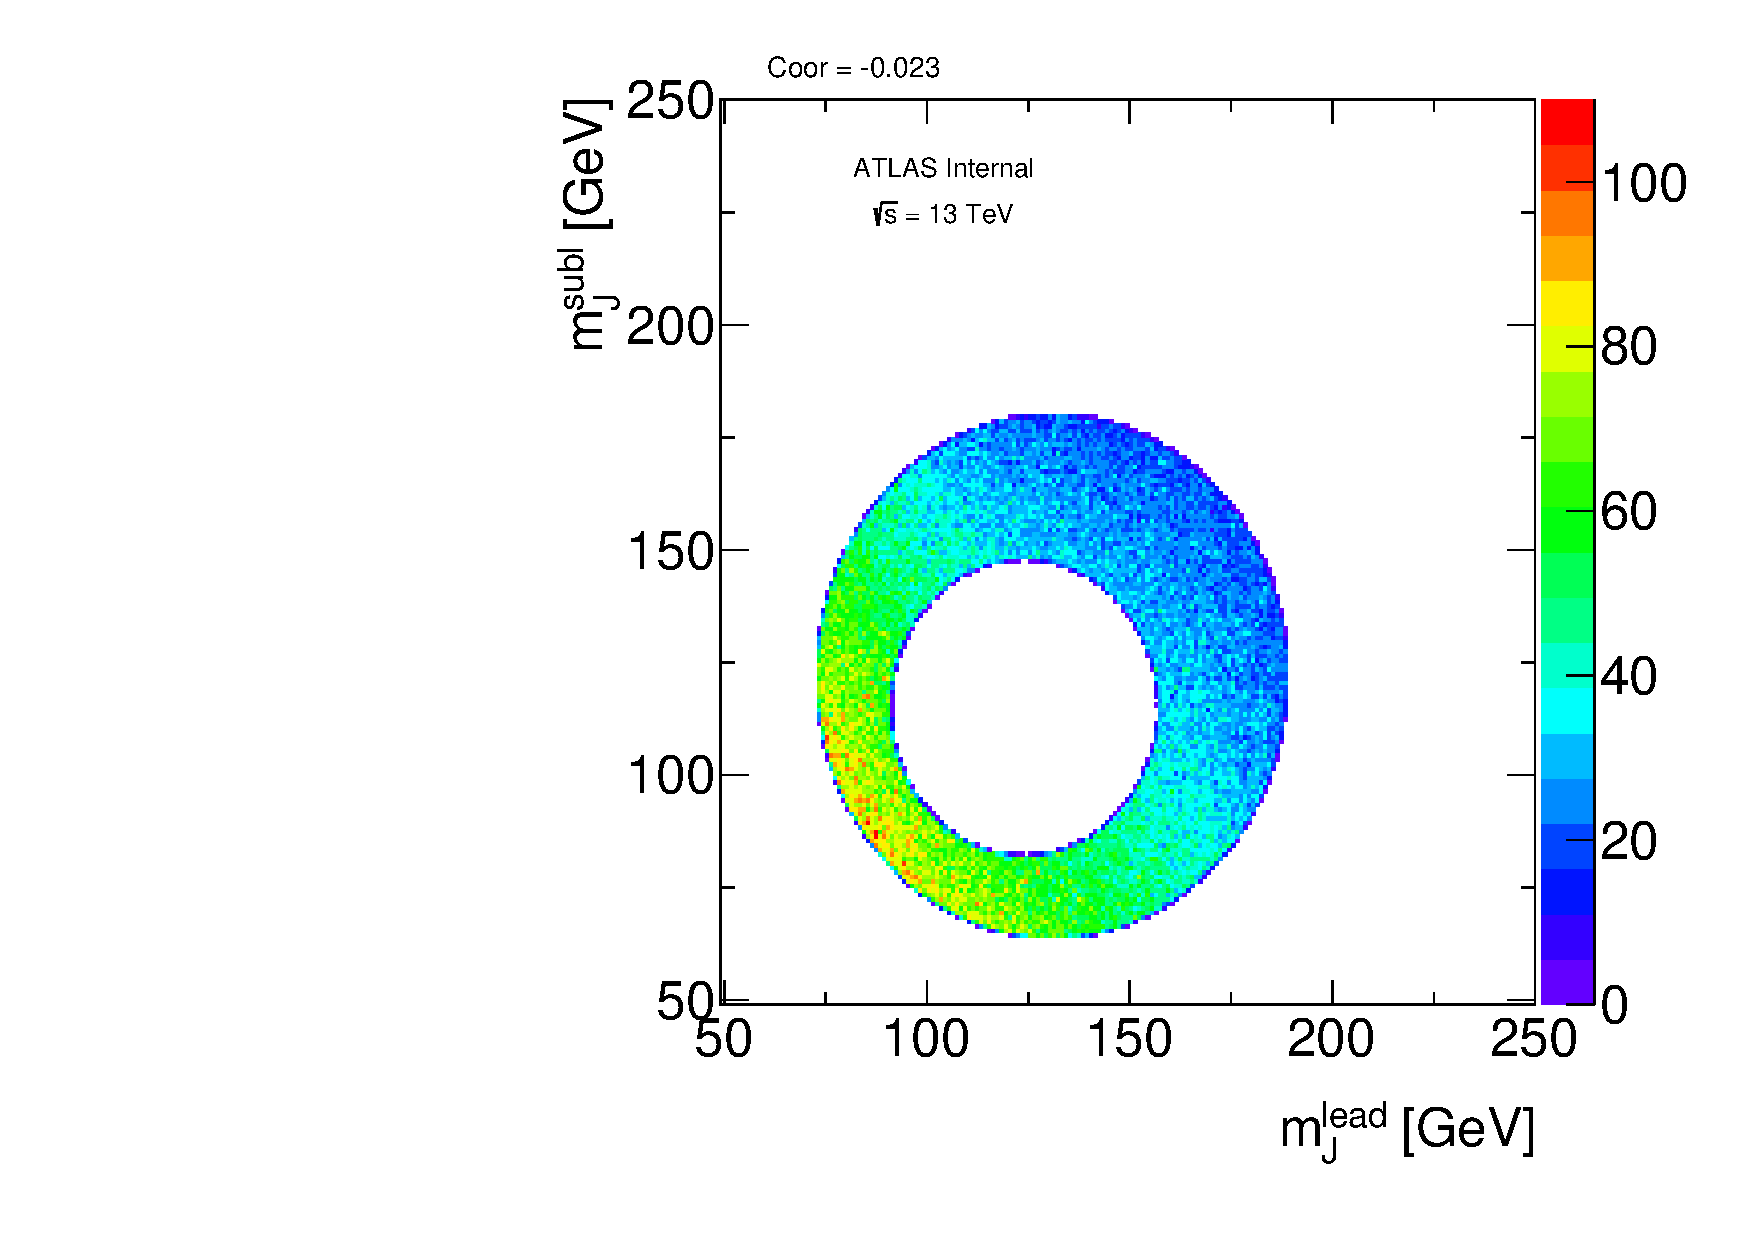
\includegraphics[width=\textwidth,angle=-90]{figures/boosted/Syst_CRSB/SB_Low_Sideband_OneTag_mH0H1.pdf}
        \caption{Sideband region}
        \label{CRSB:SB_Low_SB}
    \end{subfigure}
    \quad
    \begin{subfigure}[b]{0.39\textwidth}
        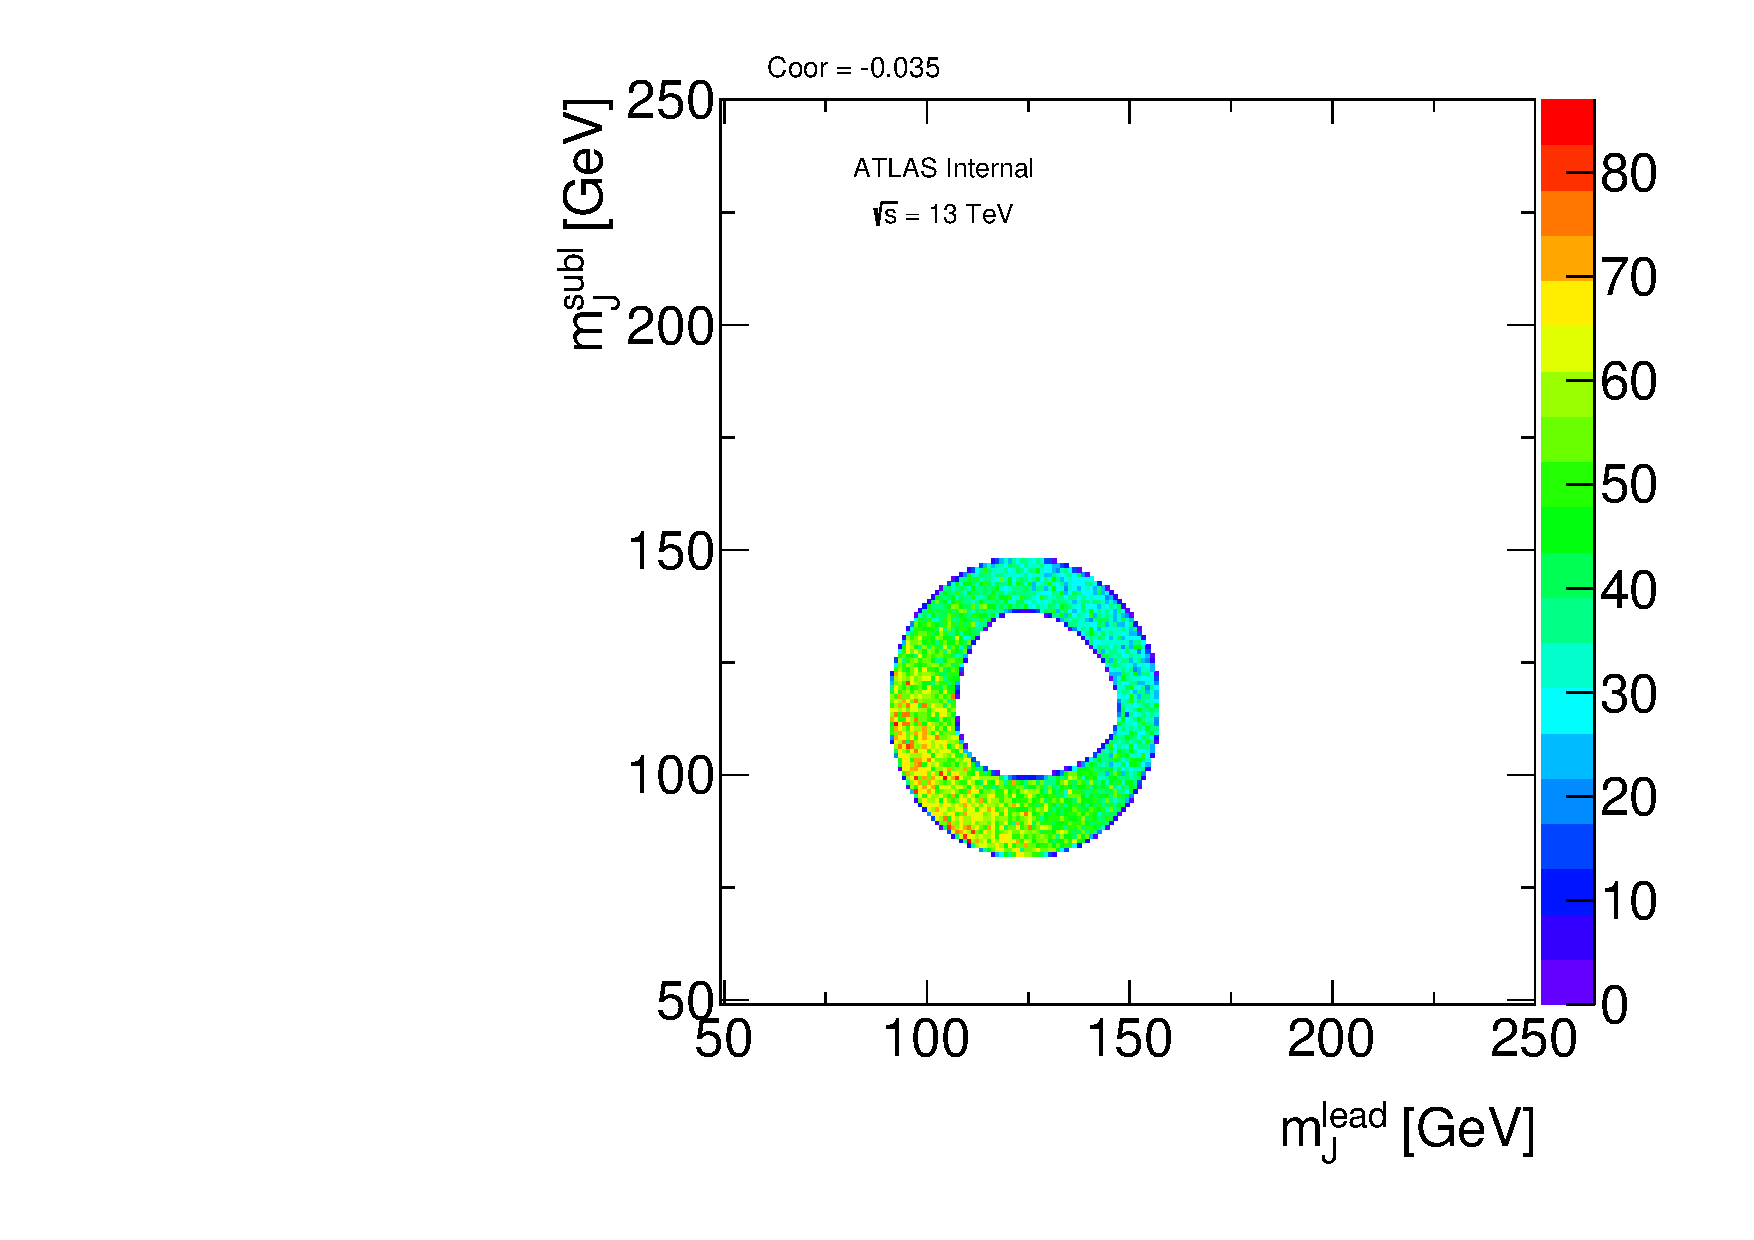
\includegraphics[width=\textwidth,angle=-90]{figures/boosted/Syst_CRSB/SB_Low_Control_OneTag_mH0H1.pdf}
        \caption{Control region}
        \label{CRSB:SB_Low_CR}
    \end{subfigure}
\caption{In $1b$ data, with the low-mass SB variation, new SB and CR \mleadJ-\msublJ~ distributions.}
\label{CRSB:SB_Low}
\end{figure}


\begin{figure}[htbp!]
\centering
\captionsetup{justification=centering}
    \begin{subfigure}[b]{0.39\textwidth}
        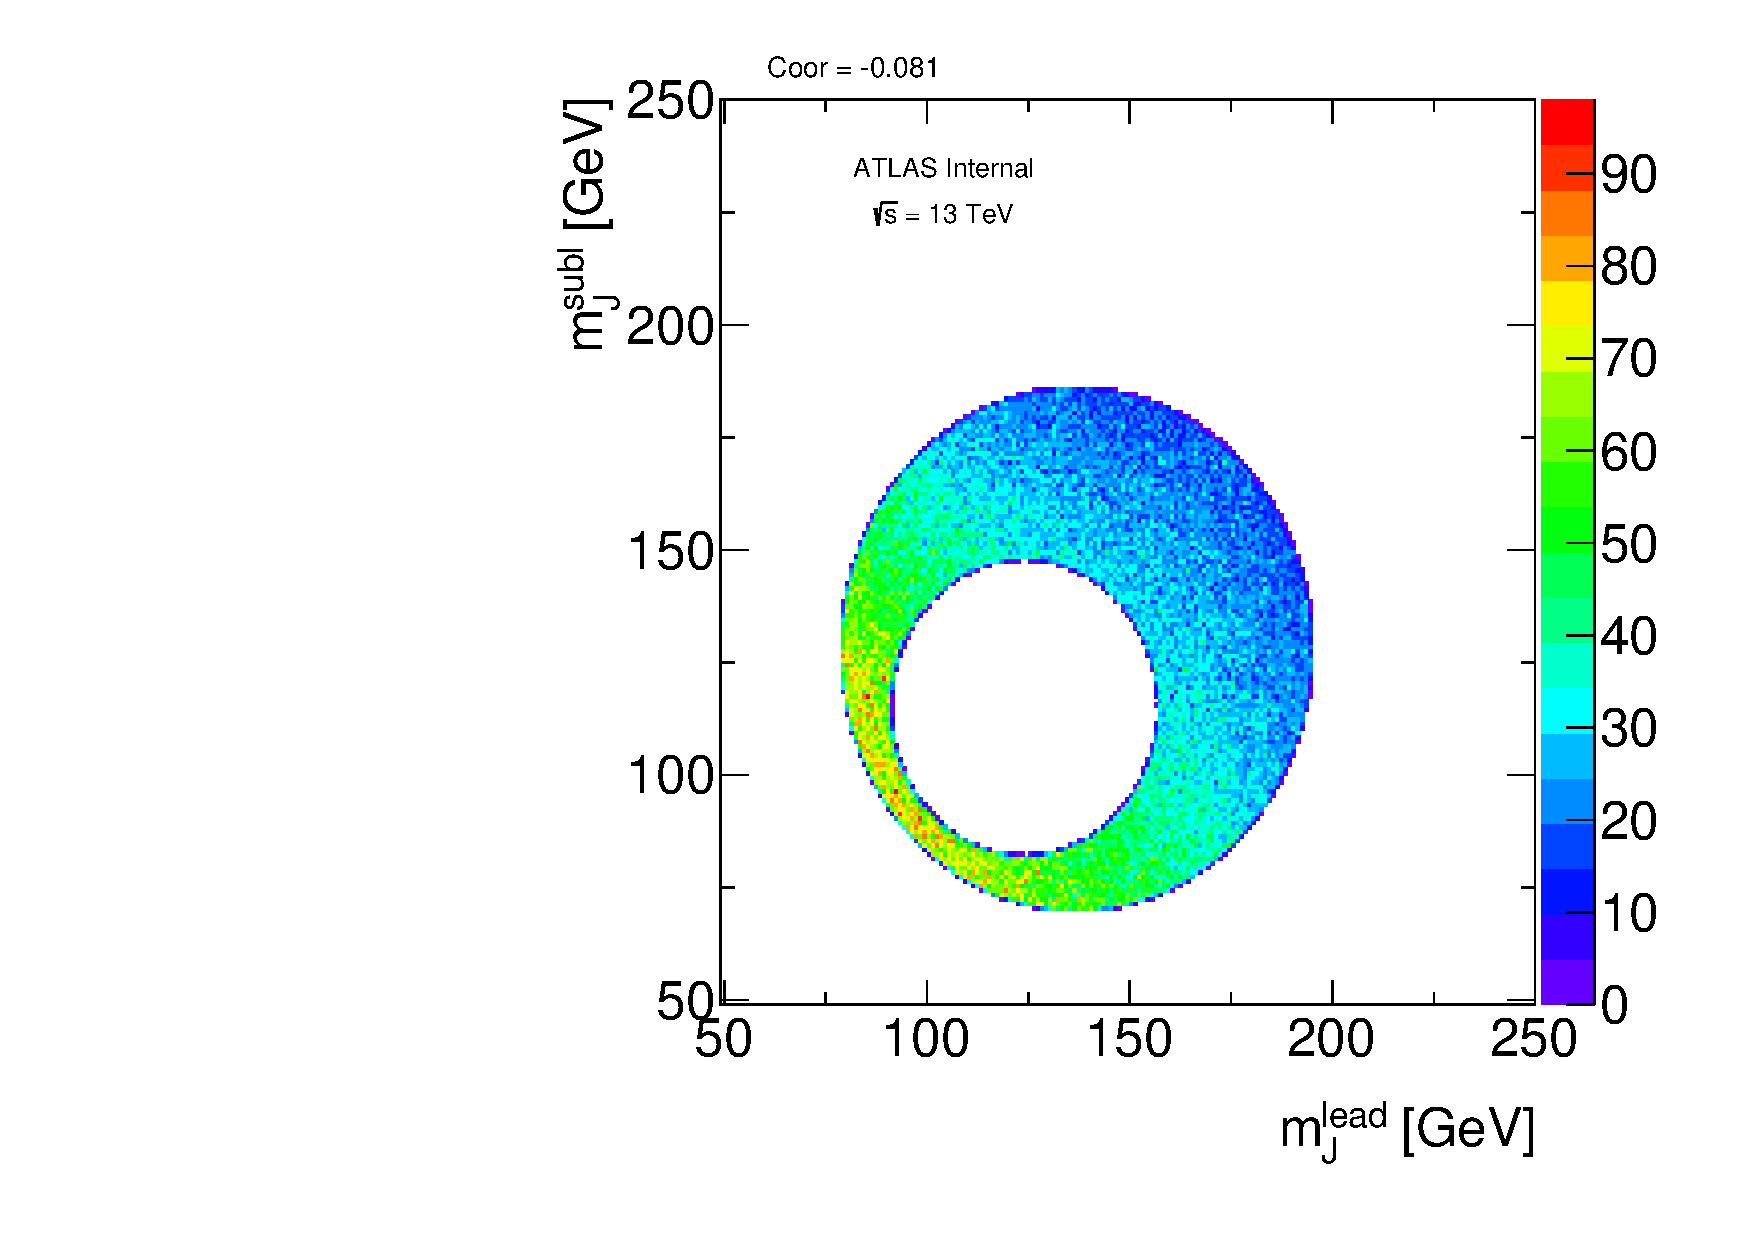
\includegraphics[width=\textwidth,angle=-90]{figures/boosted/Syst_CRSB/SB_High_Sideband_OneTag_mH0H1.pdf}
        \caption{Sideband region}
        \label{CRSB:SB_High_SB}
    \end{subfigure}
    \quad
    \begin{subfigure}[b]{0.39\textwidth}
        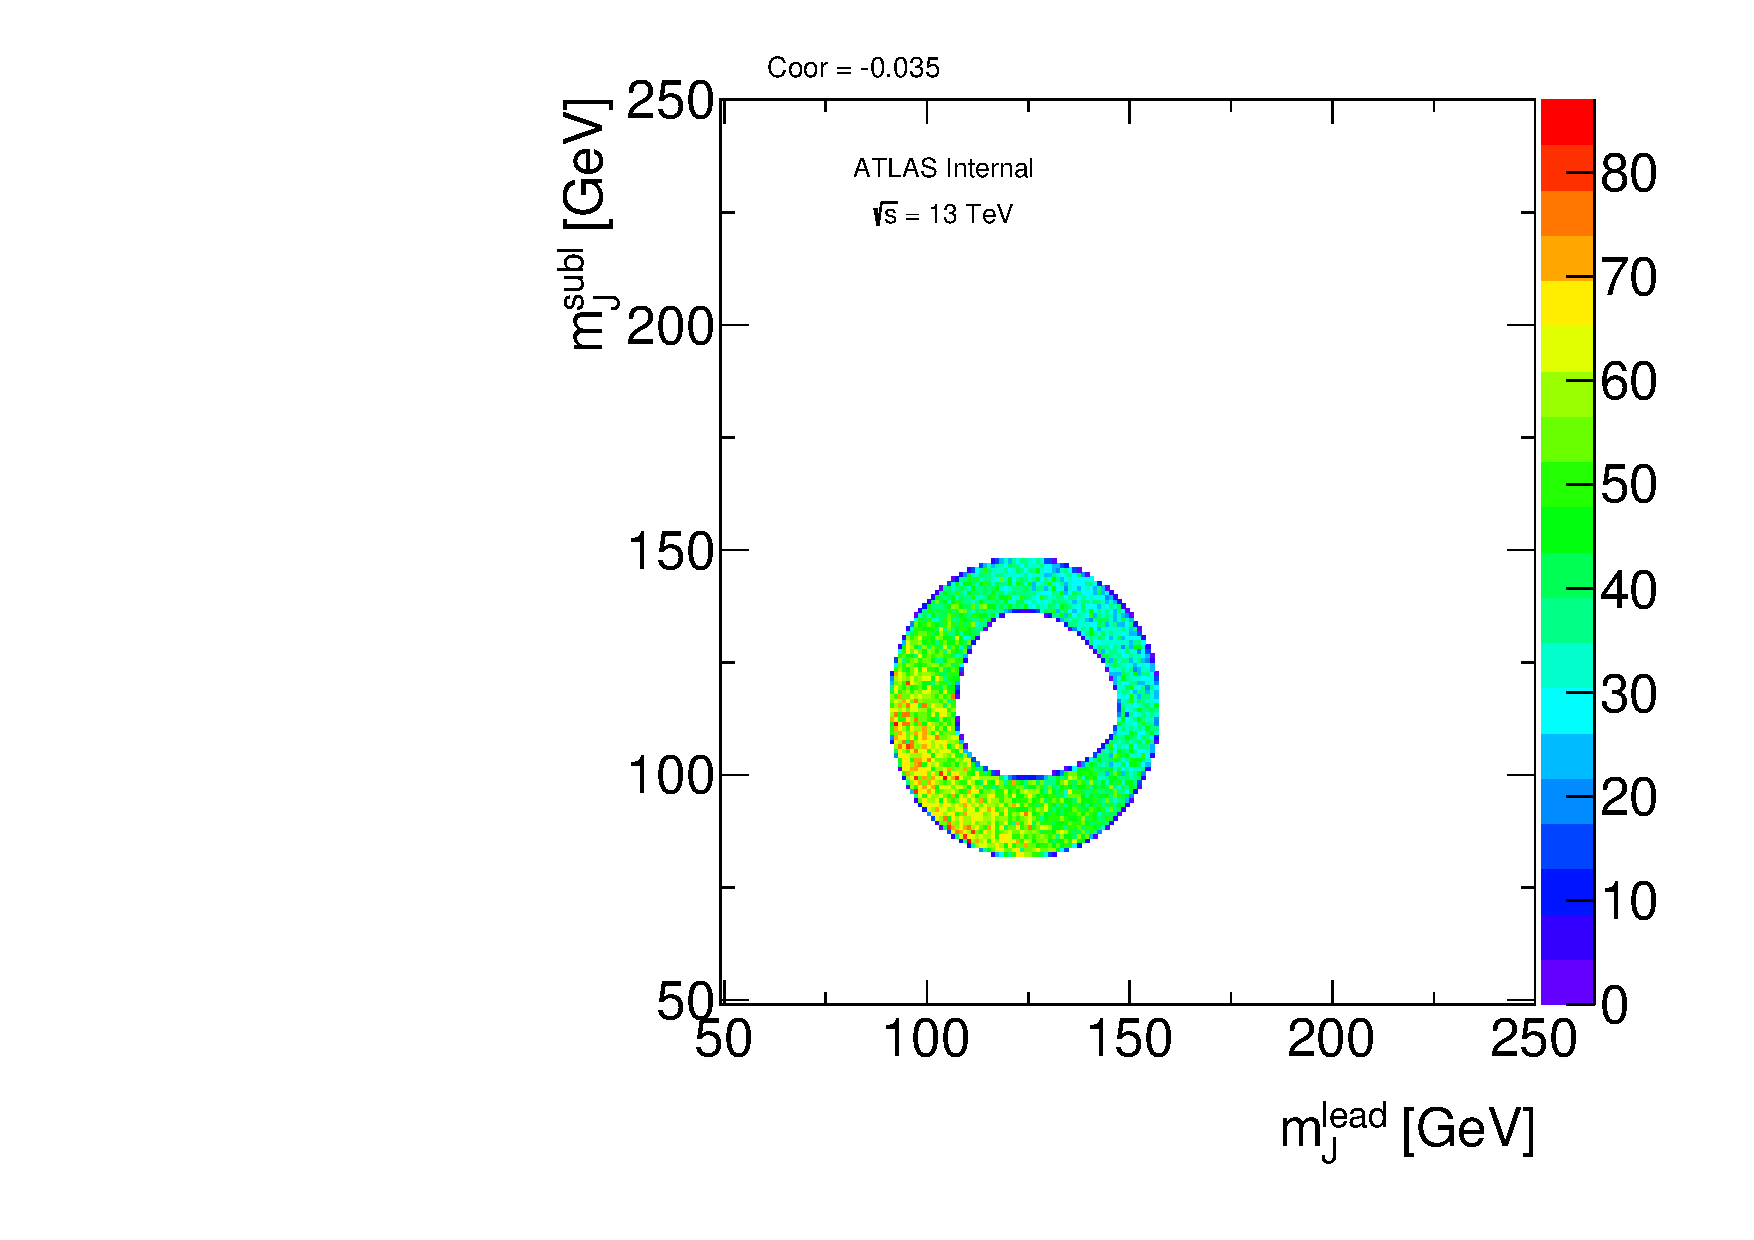
\includegraphics[width=\textwidth,angle=-90]{figures/boosted/Syst_CRSB/SB_High_Control_OneTag_mH0H1.pdf}
        \caption{Control region}
        \label{CRSB:SB_High_CR}
    \end{subfigure}
\caption{In $1b$ data, with the high-mass SB variation, new SB and CR \mleadJ-\msublJ~ distributions.}
\label{CRSB:SB_High}
\end{figure}

\begin{figure}[htbp!]
\centering
\captionsetup{justification=centering}
    \begin{subfigure}[b]{0.39\textwidth}
        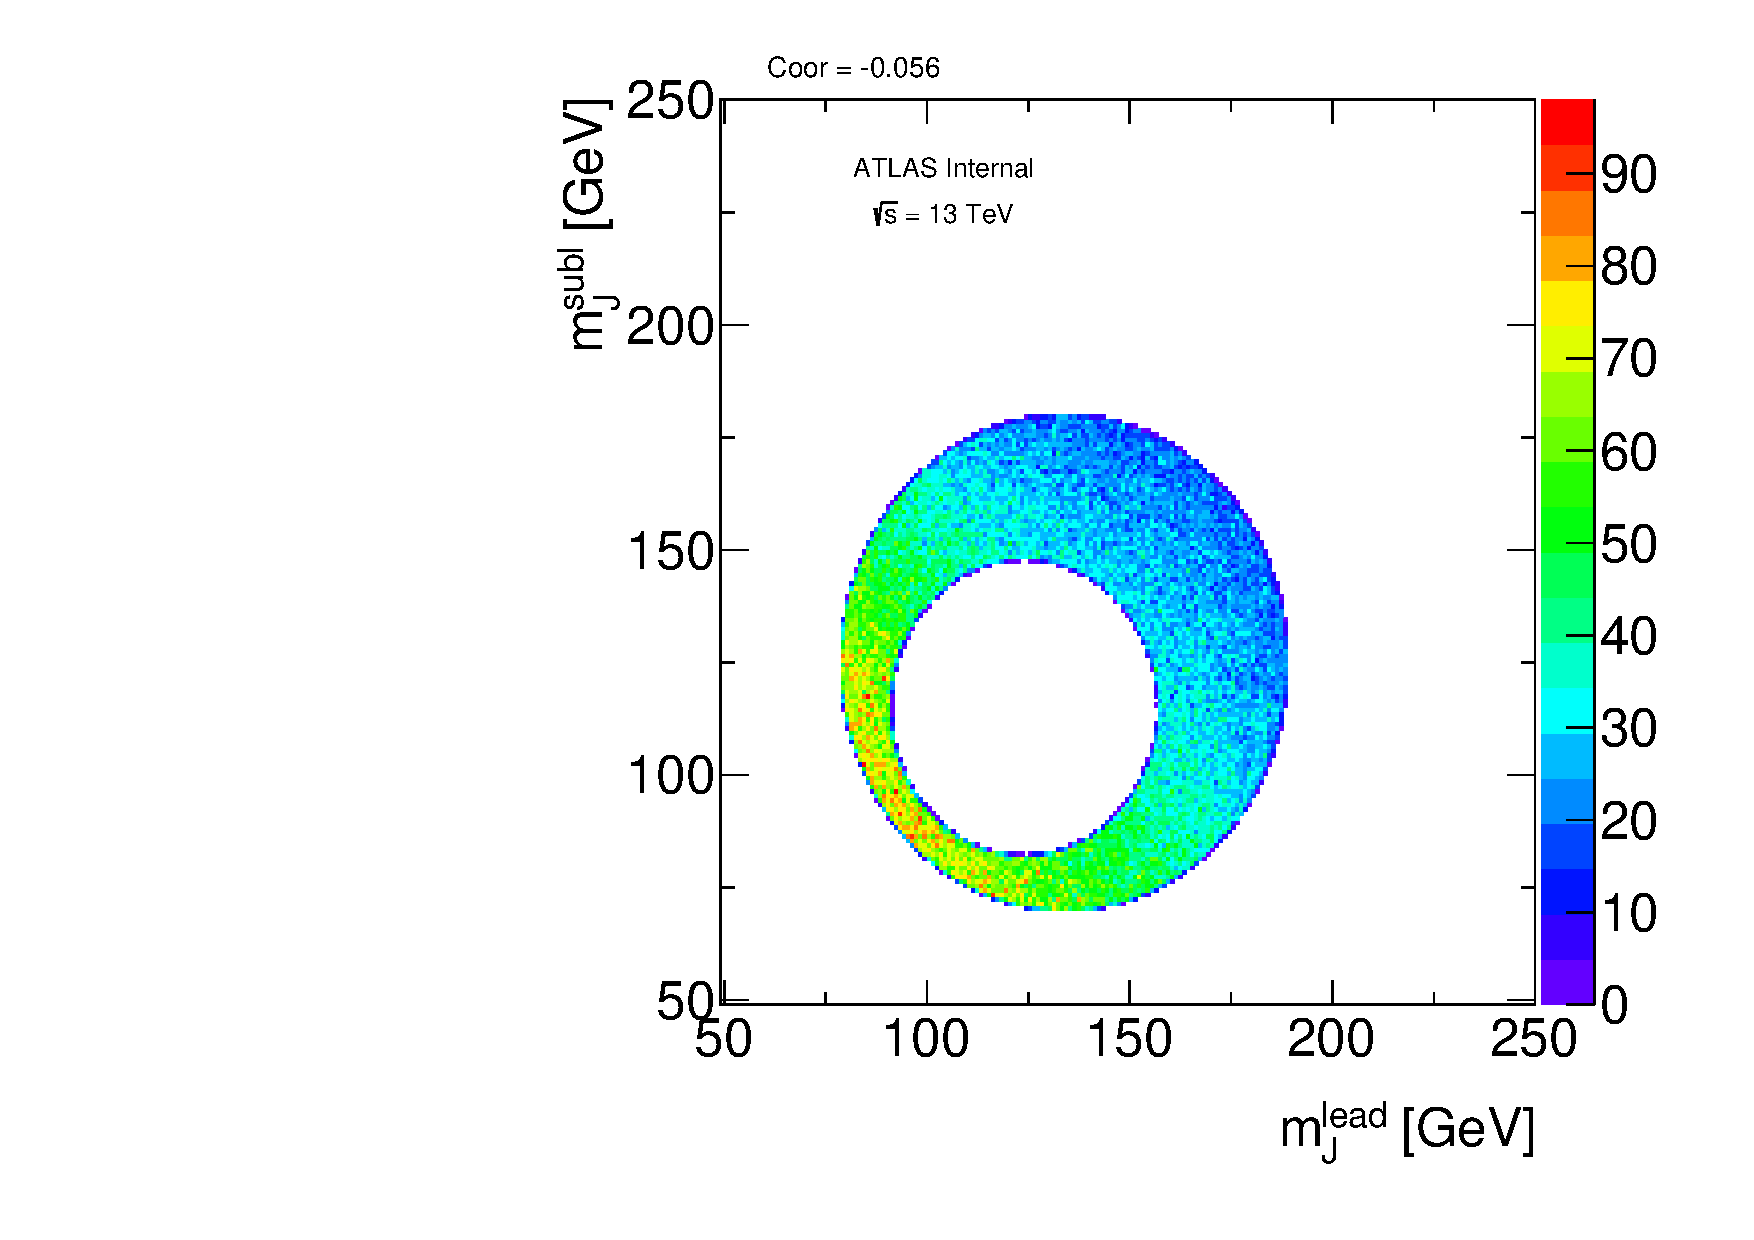
\includegraphics[width=\textwidth,angle=-90]{figures/boosted/Syst_CRSB/SB_Small_Sideband_OneTag_mH0H1.pdf}
        \caption{Sideband region}
        \label{CRSB:SB_Small_SB}
    \end{subfigure}
    \quad
    \begin{subfigure}[b]{0.39\textwidth}
        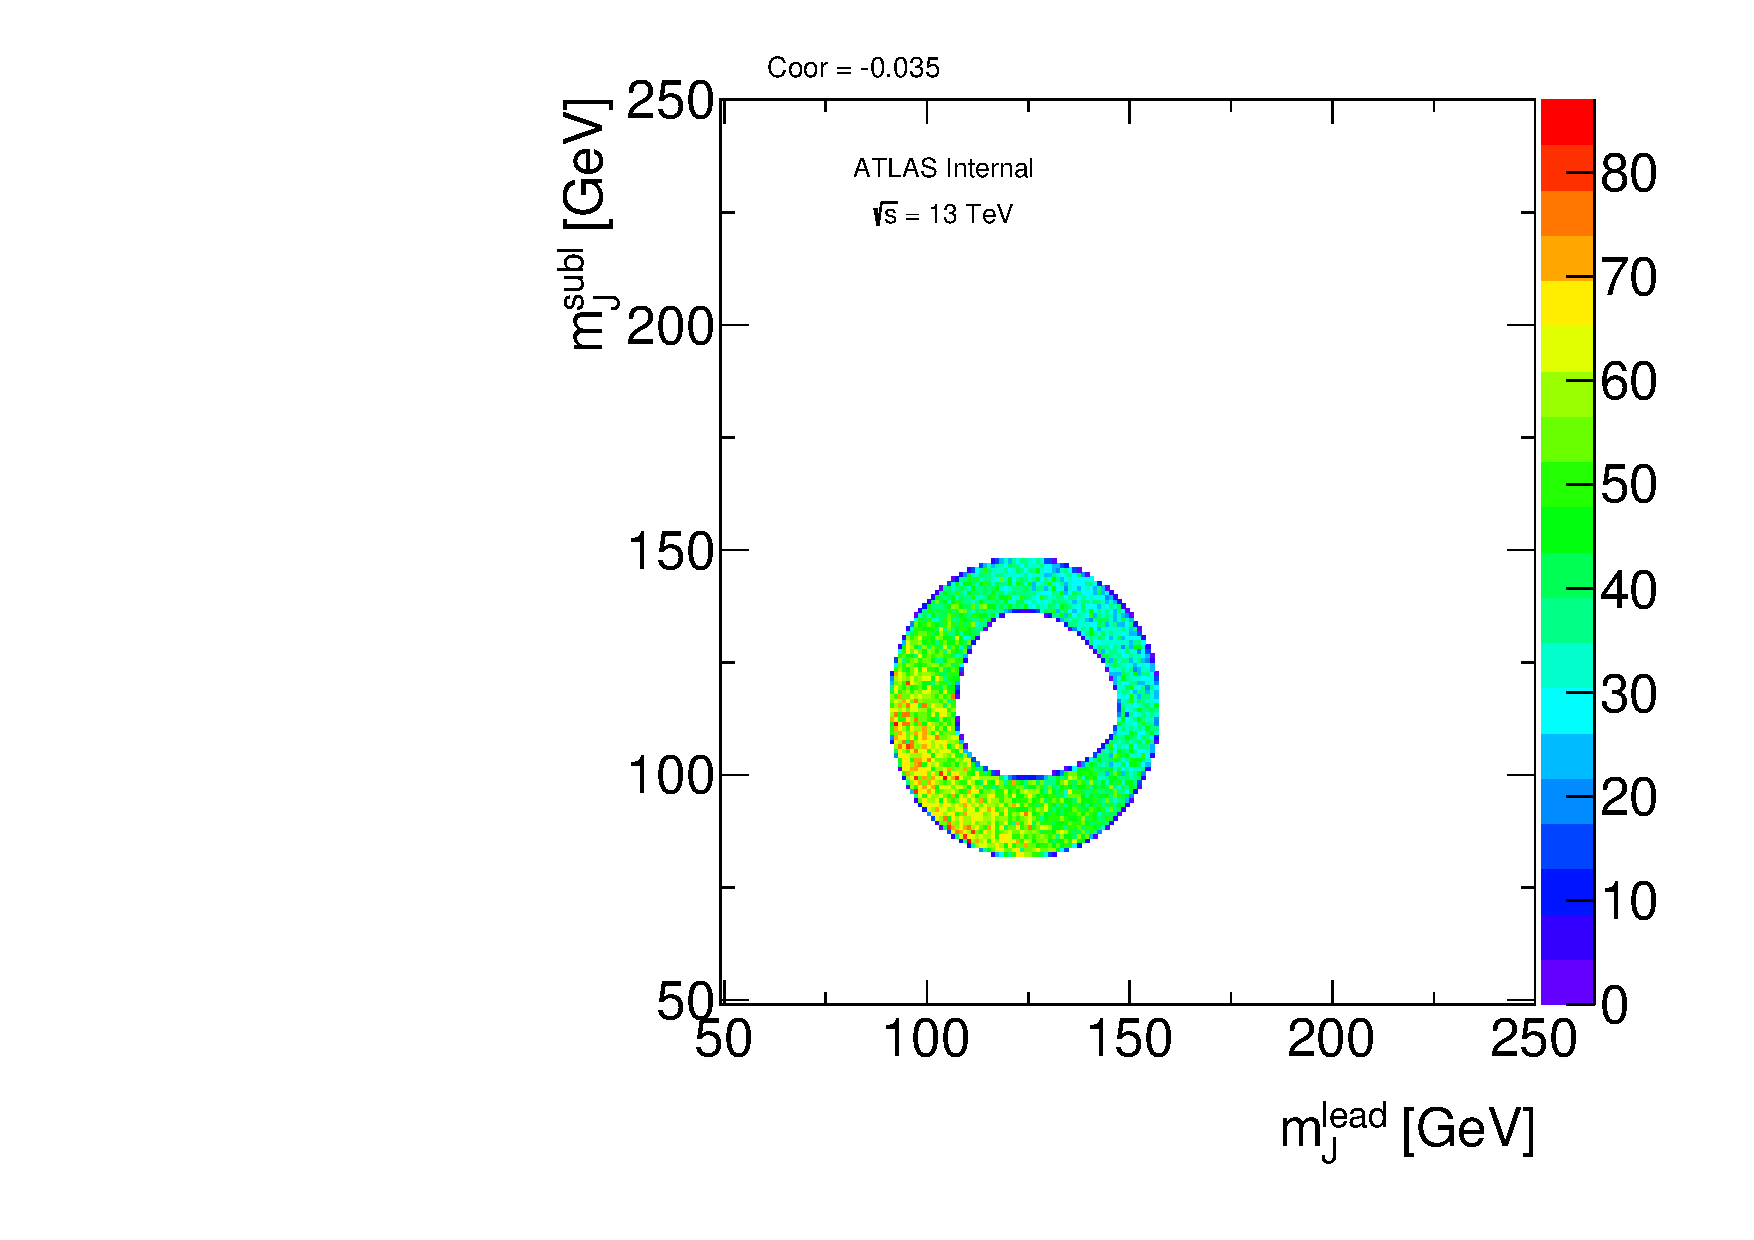
\includegraphics[width=\textwidth,angle=-90]{figures/boosted/Syst_CRSB/SB_Small_Control_OneTag_mH0H1.pdf}
        \caption{Control region}
        \label{CRSB:SB_Small_CR}
    \end{subfigure}
\caption{In $1b$ data, with the small SB variation, new SB and CR \mleadJ-\msublJ~ distributions.}
\label{CRSB:SB_Small}
\end{figure}

\begin{figure}[htbp!]
\centering
\captionsetup{justification=centering}
    \begin{subfigure}[b]{0.39\textwidth}
        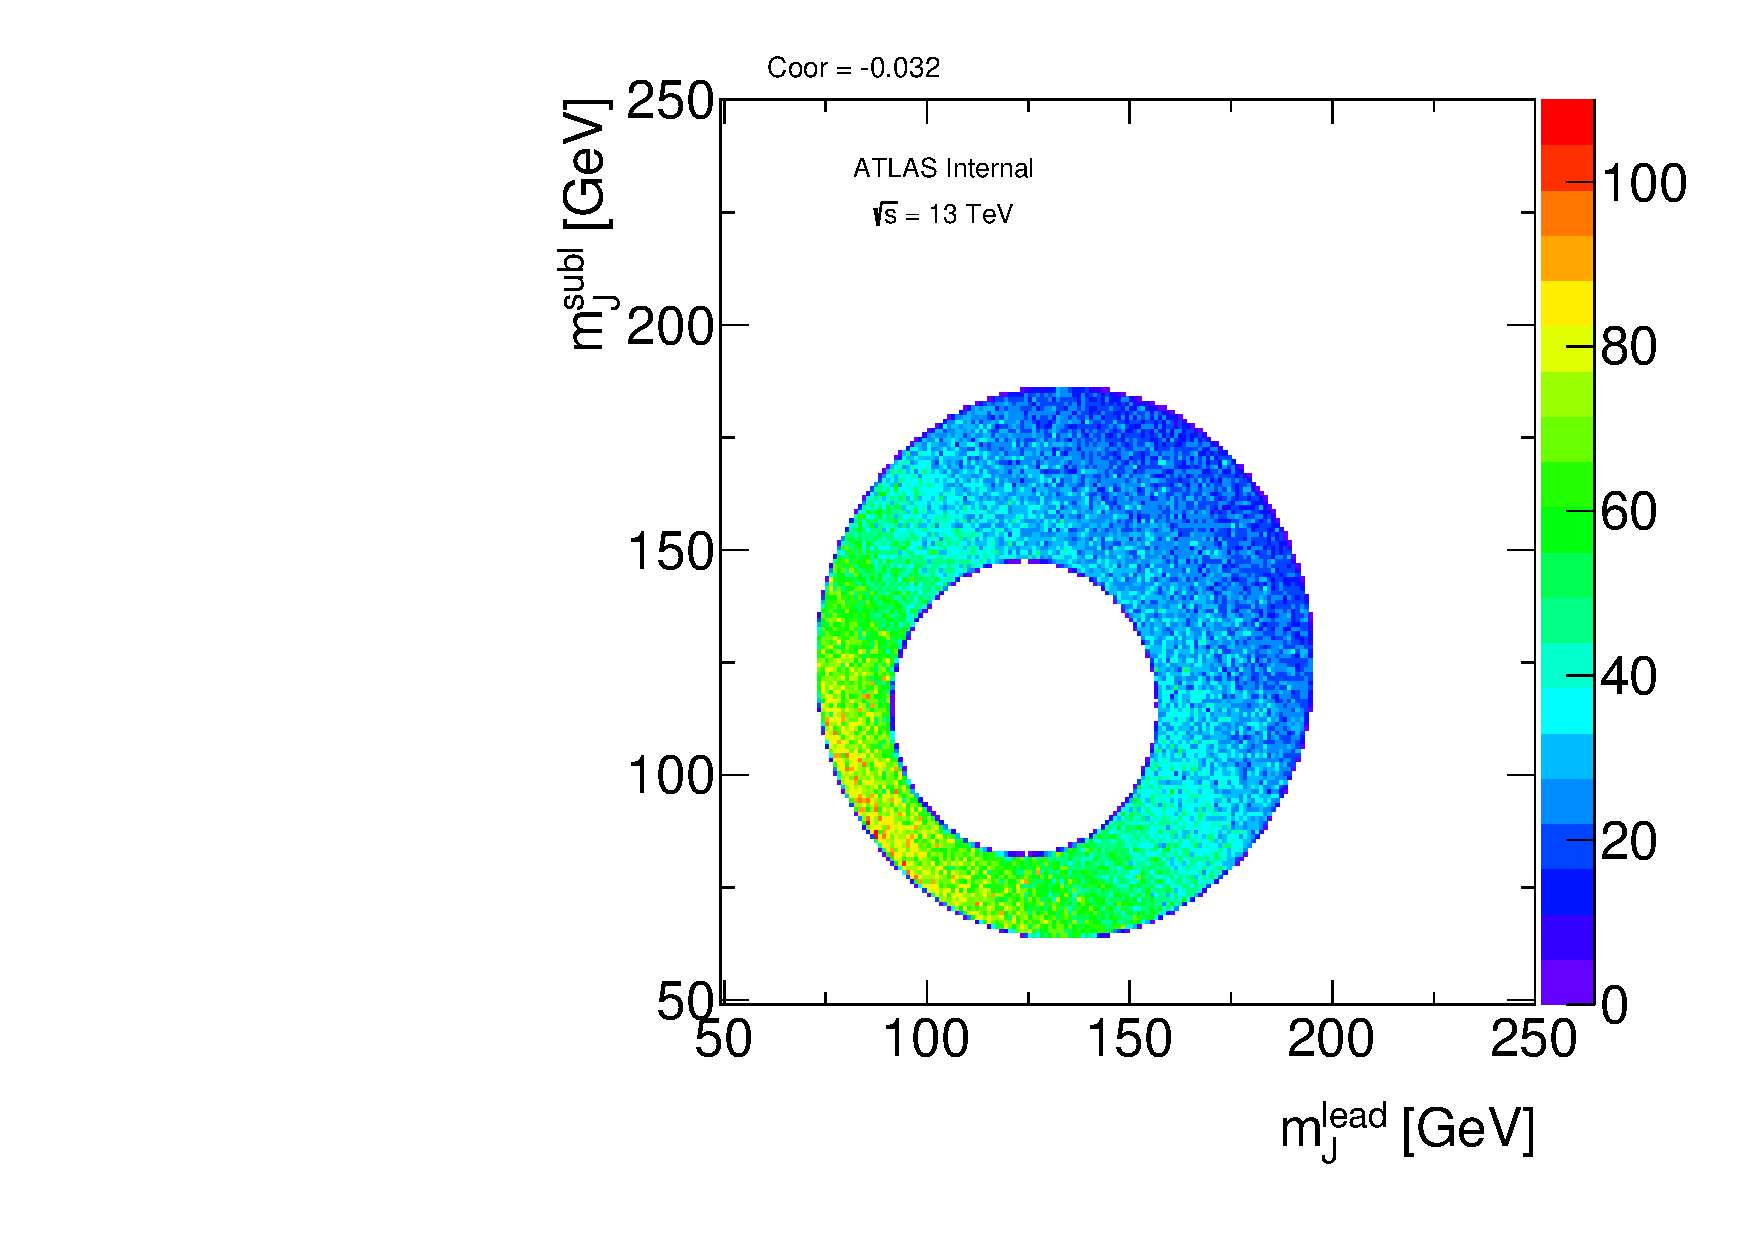
\includegraphics[width=\textwidth,angle=-90]{figures/boosted/Syst_CRSB/SB_Large_Sideband_OneTag_mH0H1.pdf}
        \caption{Sideband region}
        \label{CRSB:SB_Large_SB}
    \end{subfigure}
    \quad
    \begin{subfigure}[b]{0.39\textwidth}
        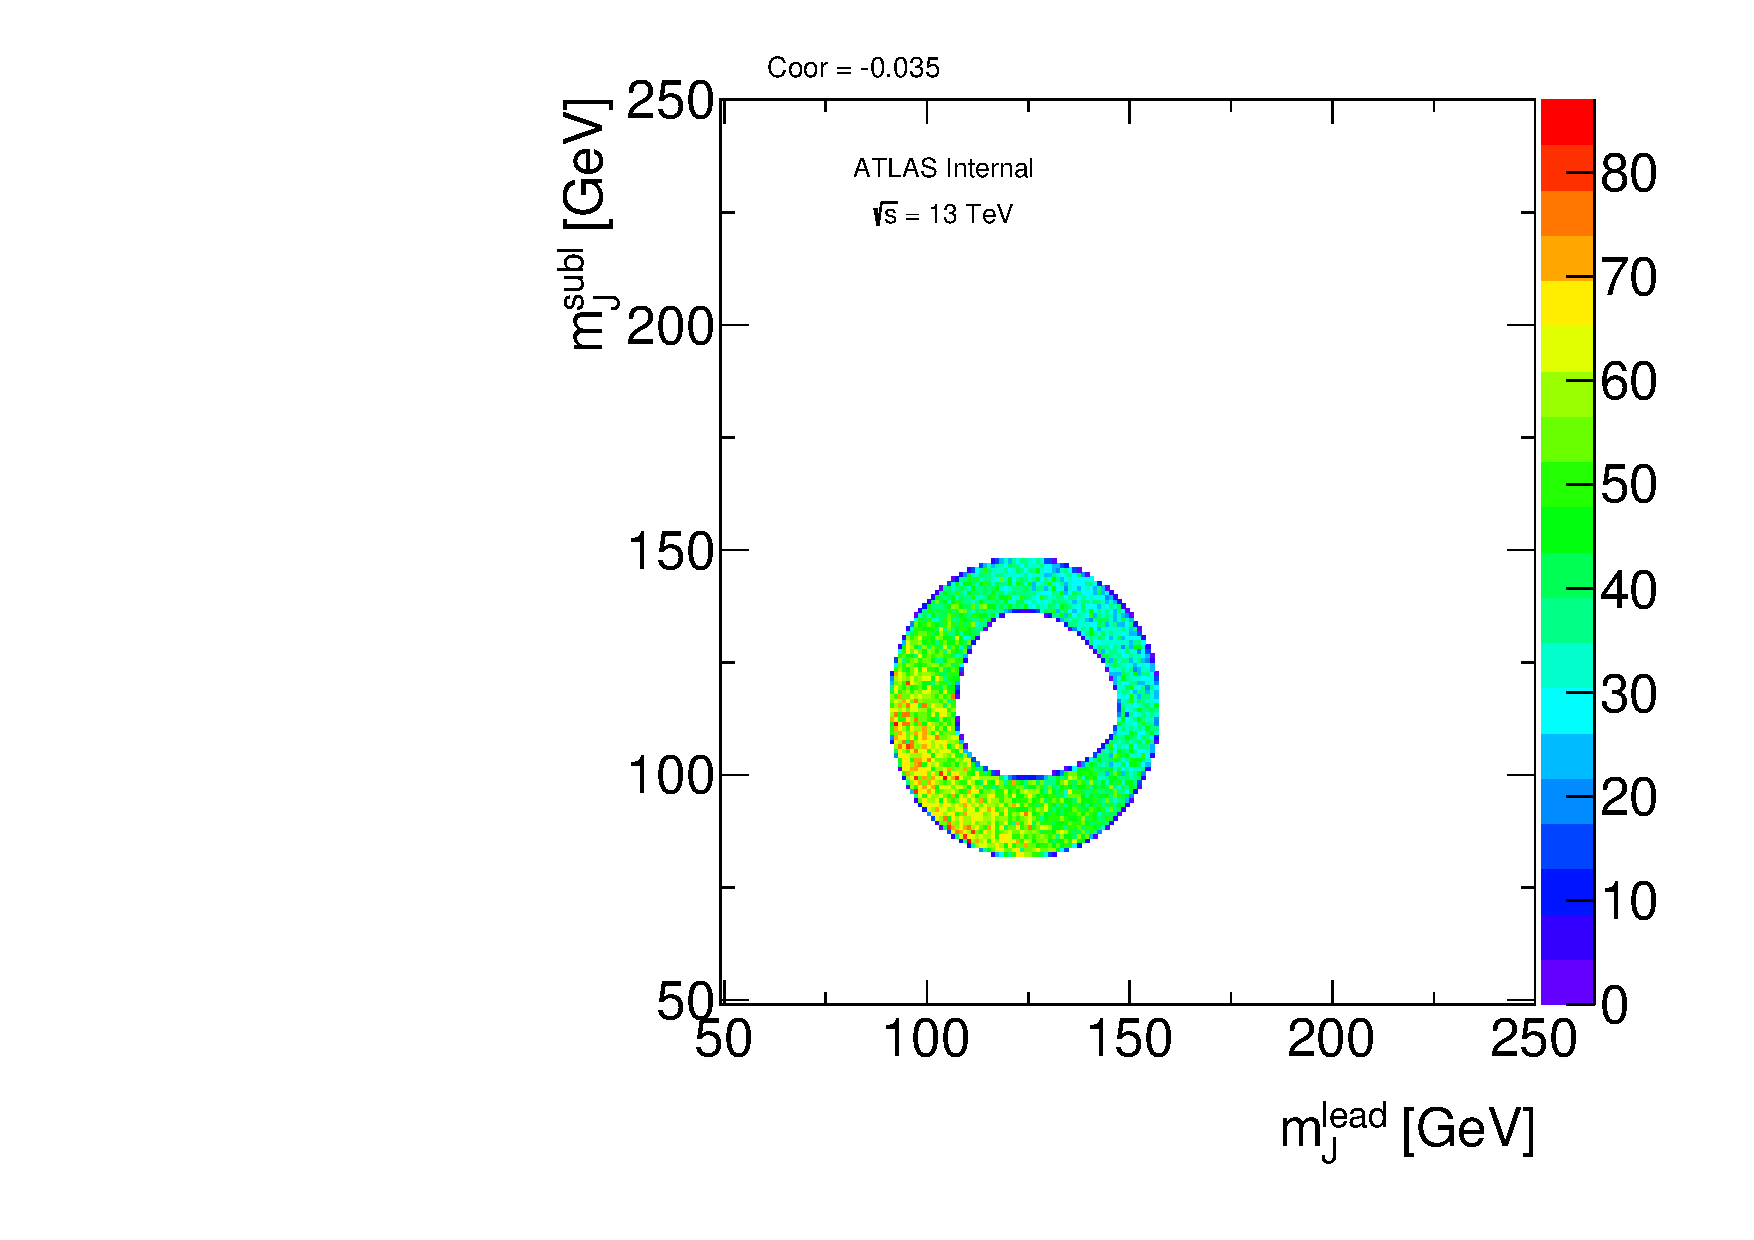
\includegraphics[width=\textwidth,angle=-90]{figures/boosted/Syst_CRSB/SB_Large_Control_OneTag_mH0H1.pdf}
        \caption{Control region}
        \label{CRSB:SB_Large_CR}
    \end{subfigure}
\caption{In $1b$ data, with the large SB variation, new SB and CR \mleadJ-\msublJ~ distributions.}
\label{CRSB:SB_Large}
\end{figure}


\clearpage
\paragraph{}
The whole background estimation procedure is repeated after the variation. Summaries of background estimated yields for $4b$ region can be found in Tables~\ref{CRSB:Tab_4b_CR_High}, \ref{CRSB:Tab_4b_CR_Low}, \ref{CRSB:Tab_4b_CR_Small}, \ref{CRSB:Tab_4b_SB_High}, \ref{CRSB:Tab_4b_SB_Low}, \ref{CRSB:Tab_4b_SB_Large}, and~\ref{CRSB:Tab_4b_SB_Small}, for each variation. 

\begin{table}[htbp!]
\begin{center}
\caption{Background prediction in SR/CR/SB for the High CR in $4b$ channel.}
\begin{footnotesize} 
\begin{tabular}{c|c|c|c} 
FourTag & Sideband & Control & Signal \\ 
\hline\hline 
& & & \\ 
QCD Est & 183.14 $\pm$ 3.02 & 58.01 $\pm$ 1.72 & 33.01 $\pm$ 1.25\\ 
$t\bar{t}$ Est.  & 25.97 $\pm$ 0.23 & 6.92 $\pm$ 0.13 & 1.62 $\pm$ 0.042\\ 
$Z+jets$ & 0 $\pm$ 0 & 6.18 $\pm$ 5.12 & 0 $\pm$ 0\\ 
Total Bkg Est & 209.12 $\pm$ 3.03 & 71.12 $\pm$ 5.41 & 34.63 $\pm$ 1.25\\ 
Data & 209.0 $\pm$ 14.46 & 76.0 $\pm$ 8.72 & 31.0 $\pm$ 5.57\\ 
$c=1.0$,$m=1.0TeV$ & 2.68 $\pm$ 0.1 & 5.23 $\pm$ 0.14 & 10.07 $\pm$ 0.2\\ 
$c=1.0$,$m=2.0TeV$ & 0.04 $\pm$ 0.0017 & 0.095 $\pm$ 0.0025 & 0.25 $\pm$ 0.0041\\ 
$c=1.0$,$m=3.0TeV$ & 0.00032 $\pm$ 3.7e-05 & 0.0008 $\pm$ 5.6e-05 & 0.0016 $\pm$ 8e-05\\ 
& & & \\ 
\hline\hline 
\end{tabular} 
\end{footnotesize} 
\newline 

\label{CRSB:Tab_4b_CR_High}
\end{center}
\end{table}

\begin{table}[htbp!]
\begin{center}
\caption{Background prediction in SR/CR/SB for the Low CR in $4b$ channel.}
\begin{footnotesize} 
\begin{tabular}{c|c|c|c} 
FourTag & Sideband & Control & Signal \\ 
\hline\hline 
QCD Est & 165.7 $\pm$ 2.84 & 69.9 $\pm$ 1.87 & 32.26 $\pm$ 1.22\\ 
$t\bar{t}$ Est.  & 28.47 $\pm$ 0.25 & 3.79 $\pm$ 0.078 & 1.59 $\pm$ 0.041\\ 
$Z+jets$ & 0 $\pm$ 0 & 6.18 $\pm$ 5.12 & 0 $\pm$ 0\\ 
Total Bkg Est & 194.17 $\pm$ 2.85 & 79.87 $\pm$ 5.45 & 33.84 $\pm$ 1.23\\ 
Data & 194.0 $\pm$ 13.93 & 91.0 $\pm$ 9.54 & 31.0 $\pm$ 5.57\\ 
$c=1.0$,$m=1.0TeV$ & 2.66 $\pm$ 0.1 & 5.26 $\pm$ 0.14 & 10.07 $\pm$ 0.2\\ 
$c=1.0$,$m=2.0TeV$ & 0.034 $\pm$ 0.0015 & 0.1 $\pm$ 0.0026 & 0.25 $\pm$ 0.0041\\ 
$c=1.0$,$m=3.0TeV$ & 0.0003 $\pm$ 3.6e-05 & 0.00082 $\pm$ 5.6e-05 & 0.0016 $\pm$ 8e-05\\ 
\hline\hline 
\end{tabular} 
\end{footnotesize} 
\newline 

\label{CRSB:Tab_4b_CR_Low}
\end{center}
\end{table}

\begin{table}[htbp!]
\caption{Background prediction in SR/CR/SB for the Small CR in $4b$ channel.}
\begin{center}
\begin{footnotesize} 
\begin{tabular}{c|c|c|c} 
FourTag & Sideband & Control & Signal \\ 
\hline\hline 
& & & \\ 
QCD Est & 176.26 $\pm$ 2.96 & 46.97 $\pm$ 1.54 & 32.91 $\pm$ 1.25\\ 
$t\bar{t}$ Est.  & 27.86 $\pm$ 0.25 & 2.81 $\pm$ 0.07 & 1.68 $\pm$ 0.044\\ 
$Z+jets$ & 0 $\pm$ 0 & 6.18 $\pm$ 5.12 & 0 $\pm$ 0\\ 
Total Bkg Est & 204.12 $\pm$ 2.97 & 55.96 $\pm$ 5.35 & 34.59 $\pm$ 1.25\\ 
Data & 204.0 $\pm$ 14.28 & 58.0 $\pm$ 7.62 & 31.0 $\pm$ 5.57\\ 
$c=1.0$,$m=1.0TeV$ & 2.52 $\pm$ 0.1 & 2.82 $\pm$ 0.11 & 10.07 $\pm$ 0.2\\ 
$c=1.0$,$m=2.0TeV$ & 0.034 $\pm$ 0.0015 & 0.054 $\pm$ 0.0019 & 0.25 $\pm$ 0.0041\\ 
$c=1.0$,$m=3.0TeV$ & 0.00032 $\pm$ 3.7e-05 & 0.00048 $\pm$ 4.3e-05 & 0.0016 $\pm$ 8e-05\\ 
& & & \\ 
\hline\hline 
\end{tabular} 
\end{footnotesize} 
\newline 

\end{center}
\label{CRSB:Tab_4b_CR_Small}
\end{table}

\begin{table}[htbp!]
\caption{Background prediction in SR/CR/SB for the High SB in $4b$ channel.}
\begin{center}
\begin{footnotesize} 
\begin{tabular}{c|c|c|c} 
FourTag & Sideband & Control & Signal \\ 
\hline\hline 
QCD Est & 168.37 $\pm$ 2.98 & 67.36 $\pm$ 1.88 & 34.53 $\pm$ 1.31\\ 
$t\bar{t}$ Est.  & 23.75 $\pm$ 0.21 & 5.18 $\pm$ 0.1 & 1.37 $\pm$ 0.035\\ 
$Z+jets$ & 0 $\pm$ 0 & 6.18 $\pm$ 5.12 & 0 $\pm$ 0\\ 
Total Bkg Est & 192.12 $\pm$ 2.99 & 78.72 $\pm$ 5.46 & 35.89 $\pm$ 1.31\\ 
Data & 192.0 $\pm$ 13.86 & 81.0 $\pm$ 9.0 & 31.0 $\pm$ 5.57\\ 
$c=1.0$,$m=1.0TeV$ & 2.46 $\pm$ 0.098 & 5.4 $\pm$ 0.15 & 10.07 $\pm$ 0.2\\ 
$c=1.0$,$m=2.0TeV$ & 0.031 $\pm$ 0.0015 & 0.1 $\pm$ 0.0026 & 0.25 $\pm$ 0.0041\\ 
$c=1.0$,$m=3.0TeV$ & 0.0003 $\pm$ 3.5e-05 & 0.0008 $\pm$ 5.6e-05 & 0.0016 $\pm$ 8e-05\\ 
\hline\hline 
\end{tabular} 
\end{footnotesize} 
\newline 

\end{center}
\label{CRSB:Tab_4b_SB_High}
\end{table}

\begin{table}[htbp!]
\caption{Background prediction in SR/CR/SB for the Low SB in $4b$ channel.}
\begin{center}
\begin{footnotesize} 
\begin{tabular}{c|c|c|c} 
FourTag & Sideband & Control & Signal \\ 
\hline\hline 
QCD Est & 176.2 $\pm$ 2.81 & 58.42 $\pm$ 1.63 & 29.95 $\pm$ 1.14\\ 
$t\bar{t}$ Est.  & 40.93 $\pm$ 0.38 & 11.91 $\pm$ 0.23 & 3.14 $\pm$ 0.081\\ 
$Z+jets$ & 0 $\pm$ 0 & 6.18 $\pm$ 5.12 & 0 $\pm$ 0\\ 
Total Bkg Est & 217.12 $\pm$ 2.84 & 76.51 $\pm$ 5.38 & 33.09 $\pm$ 1.14\\ 
Data & 217.0 $\pm$ 14.73 & 81.0 $\pm$ 9.0 & 31.0 $\pm$ 5.57\\ 
$c=1.0$,$m=1.0TeV$ & 2.52 $\pm$ 0.1 & 5.4 $\pm$ 0.15 & 10.07 $\pm$ 0.2\\ 
$c=1.0$,$m=2.0TeV$ & 0.035 $\pm$ 0.0015 & 0.1 $\pm$ 0.0026 & 0.25 $\pm$ 0.0041\\ 
$c=1.0$,$m=3.0TeV$ & 0.00033 $\pm$ 3.7e-05 & 0.0008 $\pm$ 5.6e-05 & 0.0016 $\pm$ 8e-05\\ 
\hline\hline 
\end{tabular} 
\end{footnotesize} 
\newline 

\end{center}
\label{CRSB:Tab_4b_SB_Low}
\end{table}

\begin{table}[htbp!]
\caption{Background prediction in SR/CR/SB for the Large SB in $4b$ channel.}
\begin{center}
\begin{footnotesize} 
\begin{tabular}{c|c|c|c} 
FourTag & Sideband & Control & Signal \\ 
\hline\hline 
QCD Est & 198.09 $\pm$ 3.04 & 60.63 $\pm$ 1.69 & 31.08 $\pm$ 1.18\\ 
$t\bar{t}$ Est.  & 37.04 $\pm$ 0.31 & 7.9 $\pm$ 0.16 & 2.08 $\pm$ 0.054\\ 
$Z+jets$ & 0 $\pm$ 0 & 6.18 $\pm$ 5.12 & 0 $\pm$ 0\\ 
Total Bkg Est & 235.12 $\pm$ 3.06 & 74.71 $\pm$ 5.4 & 33.16 $\pm$ 1.18\\ 
Data & 235.0 $\pm$ 15.33 & 81.0 $\pm$ 9.0 & 31.0 $\pm$ 5.57\\ 
$c=1.0$,$m=1.0TeV$ & 2.75 $\pm$ 0.1 & 5.4 $\pm$ 0.15 & 10.07 $\pm$ 0.2\\ 
$c=1.0$,$m=2.0TeV$ & 0.037 $\pm$ 0.0016 & 0.1 $\pm$ 0.0026 & 0.25 $\pm$ 0.0041\\ 
$c=1.0$,$m=3.0TeV$ & 0.00034 $\pm$ 3.8e-05 & 0.0008 $\pm$ 5.6e-05 & 0.0016 $\pm$ 8e-05\\ 
\hline\hline 
\end{tabular} 
\end{footnotesize} 
\newline 

\end{center}
\label{CRSB:Tab_4b_SB_Large}
\end{table}

\begin{table}[htbp!]
\caption{Background prediction in SR/CR/SB for the Small SB in $4b$ channel.}
\begin{center}
\begin{footnotesize} 
\begin{tabular}{c|c|c|c} 
FourTag & Sideband & Control & Signal \\ 
\hline\hline 
& & & \\ 
QCD Est & 133.42 $\pm$ 2.47 & 58.2 $\pm$ 1.63 & 29.83 $\pm$ 1.13\\ 
$t\bar{t}$ Est.  & 34.72 $\pm$ 0.33 & 9.77 $\pm$ 0.19 & 2.58 $\pm$ 0.067\\ 
$Z+jets$ & 0 $\pm$ 0 & 6.18 $\pm$ 5.12 & 0 $\pm$ 0\\ 
Total Bkg Est & 168.13 $\pm$ 2.49 & 74.15 $\pm$ 5.38 & 32.41 $\pm$ 1.13\\ 
Data & 168.0 $\pm$ 12.96 & 81.0 $\pm$ 9.0 & 31.0 $\pm$ 5.57\\ 
$c=1.0$,$m=1.0TeV$ & 2.29 $\pm$ 0.095 & 5.4 $\pm$ 0.15 & 10.07 $\pm$ 0.2\\ 
$c=1.0$,$m=2.0TeV$ & 0.03 $\pm$ 0.0014 & 0.1 $\pm$ 0.0026 & 0.25 $\pm$ 0.0041\\ 
$c=1.0$,$m=3.0TeV$ & 0.00029 $\pm$ 3.5e-05 & 0.0008 $\pm$ 5.6e-05 & 0.0016 $\pm$ 8e-05\\ 
& & & \\ 
\hline\hline 
\end{tabular} 
\end{footnotesize} 
\newline 

\end{center}
\label{CRSB:Tab_4b_SB_Small}
\end{table}
\clearpage

\paragraph{}
Summaries of background estimated yields for $3b$ region can be found in Tables~\ref{CRSB:Tab_3b_CR_High}, \ref{CRSB:Tab_3b_CR_Low}, \ref{CRSB:Tab_3b_CR_Small}, \ref{CRSB:Tab_3b_SB_High}, \ref{CRSB:Tab_3b_SB_Low}, \ref{CRSB:Tab_3b_SB_Large}, and~\ref{CRSB:Tab_3b_SB_Small}, for each variation.

\begin{table}[htbp!]
\caption{Background prediction in SR/CR/SB for the High CR in $3b$ channel.}
\begin{center}
\begin{footnotesize} 
\begin{tabular}{c|c|c|c} 
ThreeTag & Sideband & Control & Signal \\ 
\hline\hline 
QCD Est & 3632.79 $\pm$ 28.07 & 1288.95 $\pm$ 16.26 & 700.18 $\pm$ 11.93\\ 
$t\bar{t}$ Est.  & 829.13 $\pm$ 25.15 & 174.53 $\pm$ 11.64 & 78.43 $\pm$ 2.03\\ 
$Z+jets$ & 33.59 $\pm$ 11.36 & 10.42 $\pm$ 5.62 & 0.49 $\pm$ 0.49\\ 
Total Bkg Est & 4495.51 $\pm$ 39.36 & 1473.89 $\pm$ 20.77 & 779.1 $\pm$ 12.11\\ 
Data & 4495.0 $\pm$ 67.04 & 1461.0 $\pm$ 38.22 & 801.0 $\pm$ 28.3\\ 
$c=1.0$,$m=1.0TeV$ & 8.46 $\pm$ 0.19 & 11.99 $\pm$ 0.22 & 26.0 $\pm$ 0.33\\ 
$c=1.0$,$m=2.0TeV$ & 0.18 $\pm$ 0.0037 & 0.36 $\pm$ 0.0052 & 0.76 $\pm$ 0.0076\\ 
$c=1.0$,$m=3.0TeV$ & 0.0039 $\pm$ 0.00013 & 0.0072 $\pm$ 0.00018 & 0.013 $\pm$ 0.00023\\ 
\hline\hline 
\end{tabular} 
\end{footnotesize} 
\newline 

\end{center}
\label{CRSB:Tab_3b_CR_High}
\end{table}

\begin{table}[htbp!]
\caption{Background prediction in SR/CR/SB for the Low CR in $3b$ channel.}
\begin{center}
\begin{footnotesize} 
\begin{tabular}{c|c|c|c} 
ThreeTag & Sideband & Control & Signal \\ 
\hline\hline 
& & & \\ 
QCD Est & 3412.05 $\pm$ 27.11 & 1542.75 $\pm$ 18.27 & 705.03 $\pm$ 12.02\\ 
$t\bar{t}$ Est.  & 887.39 $\pm$ 26.48 & 140.33 $\pm$ 10.2 & 80.32 $\pm$ 2.08\\ 
$Z+jets$ & 29.7 $\pm$ 11.19 & 14.3 $\pm$ 5.94 & 0.49 $\pm$ 0.49\\ 
Total Bkg Est & 4329.15 $\pm$ 39.51 & 1697.38 $\pm$ 21.75 & 785.83 $\pm$ 12.2\\ 
Data & 4328.0 $\pm$ 65.79 & 1628.0 $\pm$ 40.35 & 801.0 $\pm$ 28.3\\ 
$c=1.0$,$m=1.0TeV$ & 7.87 $\pm$ 0.18 & 12.58 $\pm$ 0.23 & 26.0 $\pm$ 0.33\\ 
$c=1.0$,$m=2.0TeV$ & 0.15 $\pm$ 0.0034 & 0.39 $\pm$ 0.0054 & 0.76 $\pm$ 0.0076\\ 
$c=1.0$,$m=3.0TeV$ & 0.0036 $\pm$ 0.00013 & 0.0075 $\pm$ 0.00018 & 0.013 $\pm$ 0.00023\\ 
& & & \\ 
\hline\hline 
\end{tabular} 
\end{footnotesize} 
\newline 

\end{center}
\label{CRSB:Tab_3b_CR_Low}
\end{table}

\begin{table}[htbp!]
\caption{Background prediction in SR/CR/SB for the Small CR in $3b$ channel.}
\begin{center}
\begin{footnotesize} 
\begin{tabular}{c|c|c|c} 
ThreeTag & Sideband & Control & Signal \\ 
\hline\hline 
QCD Est & 3518.01 $\pm$ 27.48 & 1020.18 $\pm$ 14.79 & 701.6 $\pm$ 11.95\\ 
$t\bar{t}$ Est.  & 852.88 $\pm$ 25.72 & 98.31 $\pm$ 8.12 & 79.34 $\pm$ 2.05\\ 
$Z+jets$ & 32.8 $\pm$ 11.34 & 8.84 $\pm$ 5.19 & 0.49 $\pm$ 0.49\\ 
Total Bkg Est & 4403.69 $\pm$ 39.31 & 1127.34 $\pm$ 17.66 & 781.42 $\pm$ 12.14\\ 
Data & 4403.0 $\pm$ 66.36 & 1134.0 $\pm$ 33.67 & 801.0 $\pm$ 28.3\\ 
$c=1.0$,$m=1.0TeV$ & 7.86 $\pm$ 0.18 & 7.5 $\pm$ 0.18 & 26.0 $\pm$ 0.33\\ 
$c=1.0$,$m=2.0TeV$ & 0.16 $\pm$ 0.0035 & 0.22 $\pm$ 0.0041 & 0.76 $\pm$ 0.0076\\ 
$c=1.0$,$m=3.0TeV$ & 0.0036 $\pm$ 0.00013 & 0.0043 $\pm$ 0.00014 & 0.013 $\pm$ 0.00023\\ 
\hline\hline 
\end{tabular} 
\end{footnotesize} 
\newline 

\end{center}
\label{CRSB:Tab_3b_CR_Small}
\end{table}

\begin{table}[htbp!]
\caption{Background prediction in SR/CR/SB for the High SB in $3b$ channel.}
\begin{center}
\begin{footnotesize} 
\begin{tabular}{c|c|c|c} 
ThreeTag & Sideband & Control & Signal \\ 
\hline\hline 
& & & \\ 
QCD Est & 3244.66 $\pm$ 26.66 & 1431.35 $\pm$ 17.56 & 710.47 $\pm$ 12.09\\ 
$t\bar{t}$ Est.  & 889.75 $\pm$ 26.15 & 160.18 $\pm$ 11.01 & 78.3 $\pm$ 2.03\\ 
$Z+jets$ & 28.07 $\pm$ 10.31 & 11.21 $\pm$ 5.65 & 0.49 $\pm$ 0.49\\ 
Total Bkg Est & 4162.48 $\pm$ 38.74 & 1602.74 $\pm$ 21.48 & 789.26 $\pm$ 12.27\\ 
Data & 4162.0 $\pm$ 64.51 & 1553.0 $\pm$ 39.41 & 801.0 $\pm$ 28.3\\ 
$c=1.0$,$m=1.0TeV$ & 7.55 $\pm$ 0.18 & 12.58 $\pm$ 0.23 & 26.0 $\pm$ 0.33\\ 
$c=1.0$,$m=2.0TeV$ & 0.14 $\pm$ 0.0033 & 0.38 $\pm$ 0.0054 & 0.76 $\pm$ 0.0076\\ 
$c=1.0$,$m=3.0TeV$ & 0.0032 $\pm$ 0.00012 & 0.0075 $\pm$ 0.00018 & 0.013 $\pm$ 0.00023\\ 
& & & \\ 
\hline\hline 
\end{tabular} 
\end{footnotesize} 
\newline 

\end{center}
\label{CRSB:Tab_3b_SB_High}
\end{table}

\begin{table}[htbp!]
\caption{Background prediction in SR/CR/SB for the Low SB in $3b$ channel.}
\begin{center}
\begin{footnotesize} 
\begin{tabular}{c|c|c|c} 
ThreeTag & Sideband & Control & Signal \\ 
\hline\hline 
& & & \\ 
QCD Est & 3797.02 $\pm$ 28.24 & 1395.42 $\pm$ 17.15 & 692.6 $\pm$ 11.8\\ 
$t\bar{t}$ Est.  & 825.52 $\pm$ 25.8 & 169.94 $\pm$ 11.68 & 83.07 $\pm$ 2.15\\ 
$Z+jets$ & 50.5 $\pm$ 15.32 & 11.21 $\pm$ 5.65 & 0.49 $\pm$ 0.49\\ 
Total Bkg Est & 4673.04 $\pm$ 41.2 & 1576.56 $\pm$ 21.5 & 776.15 $\pm$ 12.01\\ 
Data & 4672.0 $\pm$ 68.35 & 1553.0 $\pm$ 39.41 & 801.0 $\pm$ 28.3\\ 
$c=1.0$,$m=1.0TeV$ & 8.09 $\pm$ 0.18 & 12.58 $\pm$ 0.23 & 26.0 $\pm$ 0.33\\ 
$c=1.0$,$m=2.0TeV$ & 0.17 $\pm$ 0.0036 & 0.38 $\pm$ 0.0054 & 0.76 $\pm$ 0.0076\\ 
$c=1.0$,$m=3.0TeV$ & 0.0039 $\pm$ 0.00013 & 0.0075 $\pm$ 0.00018 & 0.013 $\pm$ 0.00023\\ 
& & & \\ 
\hline\hline 
\end{tabular} 
\end{footnotesize} 
\newline 

\end{center}
\label{CRSB:Tab_3b_SB_Low}
\end{table}

\begin{table}[htbp!]
\caption{Background prediction in SR/CR/SB for the Large SB in $3b$ channel.}
\begin{center}
\begin{footnotesize} 
\begin{tabular}{c|c|c|c} 
ThreeTag & Sideband & Control & Signal \\ 
\hline\hline 
QCD Est & 4094.15 $\pm$ 29.34 & 1392.94 $\pm$ 17.09 & 691.4 $\pm$ 11.77\\ 
$t\bar{t}$ Est.  & 993.33 $\pm$ 28.3 & 170.09 $\pm$ 11.69 & 83.14 $\pm$ 2.15\\ 
$Z+jets$ & 44.81 $\pm$ 13.44 & 11.21 $\pm$ 5.65 & 0.49 $\pm$ 0.49\\ 
Total Bkg Est & 5132.28 $\pm$ 42.92 & 1574.23 $\pm$ 21.47 & 775.03 $\pm$ 11.97\\ 
Data & 5132.0 $\pm$ 71.64 & 1553.0 $\pm$ 39.41 & 801.0 $\pm$ 28.3\\ 
$c=1.0$,$m=1.0TeV$ & 8.63 $\pm$ 0.19 & 12.58 $\pm$ 0.23 & 26.0 $\pm$ 0.33\\ 
$c=1.0$,$m=2.0TeV$ & 0.18 $\pm$ 0.0037 & 0.38 $\pm$ 0.0054 & 0.76 $\pm$ 0.0076\\ 
$c=1.0$,$m=3.0TeV$ & 0.0039 $\pm$ 0.00013 & 0.0075 $\pm$ 0.00018 & 0.013 $\pm$ 0.00023\\ 
\hline\hline 
\end{tabular} 
\end{footnotesize} 
\newline 

\end{center}
\label{CRSB:Tab_3b_SB_Large}
\end{table}

\begin{table}[htbp!]
\caption{Background prediction in SR/CR/SB for the Small SB in $3b$ channel.}
\begin{center}
\begin{footnotesize} 
\begin{tabular}{c|c|c|c} 
ThreeTag & Sideband & Control & Signal \\ 
\hline\hline 
& & & \\ 
QCD Est & 2935.02 $\pm$ 25.3 & 1424.16 $\pm$ 17.5 & 706.86 $\pm$ 12.05\\ 
$t\bar{t}$ Est.  & 765.58 $\pm$ 24.63 & 166.07 $\pm$ 11.41 & 81.18 $\pm$ 2.1\\ 
$Z+jets$ & 28.07 $\pm$ 10.31 & 11.21 $\pm$ 5.65 & 0.49 $\pm$ 0.49\\ 
Total Bkg Est & 3728.68 $\pm$ 36.78 & 1601.44 $\pm$ 21.64 & 788.53 $\pm$ 12.24\\ 
Data & 3728.0 $\pm$ 61.06 & 1553.0 $\pm$ 39.41 & 801.0 $\pm$ 28.3\\ 
$c=1.0$,$m=1.0TeV$ & 7.03 $\pm$ 0.17 & 12.58 $\pm$ 0.23 & 26.0 $\pm$ 0.33\\ 
$c=1.0$,$m=2.0TeV$ & 0.14 $\pm$ 0.0033 & 0.38 $\pm$ 0.0054 & 0.76 $\pm$ 0.0076\\ 
$c=1.0$,$m=3.0TeV$ & 0.0032 $\pm$ 0.00012 & 0.0075 $\pm$ 0.00018 & 0.013 $\pm$ 0.00023\\ 
& & & \\ 
\hline\hline 
\end{tabular} 
\end{footnotesize} 
\newline 

\end{center}
\label{CRSB:Tab_3b_SB_Small}
\end{table}
\clearpage

\paragraph{}
Summaries of background estimated yields for $2bs$ region can be found in Tables~\ref{CRSB:Tab_2bs_CR_High}, \ref{CRSB:Tab_2bs_CR_Low}, \ref{CRSB:Tab_2bs_CR_Small}, \ref{CRSB:Tab_2bs_SB_High}, \ref{CRSB:Tab_2bs_SB_Low}, \ref{CRSB:Tab_2bs_SB_Large}, and~\ref{CRSB:Tab_2bs_SB_Small}, for each variation.

\begin{table}[htbp!]
\caption{Background prediction in SR/CR/SB for the High CR in $2bs$ channel.}
\begin{center}
\begin{footnotesize} 
\begin{tabular}{c|c|c|c} 
TwoTag split & Sideband & Control & Signal \\ 
\hline\hline 
& & & \\ 
QCD Est & 17680.28 $\pm$ 38.67 & 6283.4 $\pm$ 22.64 & 3382.9 $\pm$ 16.59\\ 
$t\bar{t}$ Est.  & 7700.3 $\pm$ 69.5 & 1629.22 $\pm$ 30.95 & 857.59 $\pm$ 22.21\\ 
$Z+jets$ & 69.2 $\pm$ 16.9 & 24.98 $\pm$ 9.93 & 0.13 $\pm$ 0.091\\ 
Total Bkg Est & 25449.78 $\pm$ 81.31 & 7937.59 $\pm$ 39.61 & 4240.62 $\pm$ 27.72\\ 
Data & 25449.0 $\pm$ 159.53 & 8174.0 $\pm$ 90.41 & 4376.0 $\pm$ 66.15\\ 
$c=1.0$,$m=1.0TeV$ & 5.21 $\pm$ 0.15 & 5.91 $\pm$ 0.16 & 10.87 $\pm$ 0.22\\ 
$c=1.0$,$m=2.0TeV$ & 0.21 $\pm$ 0.0042 & 0.34 $\pm$ 0.0054 & 0.6 $\pm$ 0.0072\\ 
$c=1.0$,$m=3.0TeV$ & 0.015 $\pm$ 0.00026 & 0.025 $\pm$ 0.00034 & 0.039 $\pm$ 0.00041\\ 
& & & \\ 
\hline\hline 
\end{tabular} 
\end{footnotesize} 
\newline 

\end{center}
\label{CRSB:Tab_2bs_CR_High}
\end{table}

\begin{table}[htbp!]
\caption{Background prediction in SR/CR/SB for the Low CR in $2bs$ channel.}
\begin{center}
\begin{footnotesize} 
\begin{tabular}{c|c|c|c} 
TwoTag split & Sideband & Control & Signal \\ 
\hline\hline 
& & & \\ 
QCD Est & 16635.37 $\pm$ 37.77 & 7376.46 $\pm$ 24.35 & 3390.48 $\pm$ 16.64\\ 
$t\bar{t}$ Est.  & 8026.21 $\pm$ 71.28 & 1385.31 $\pm$ 28.45 & 865.13 $\pm$ 22.4\\ 
$Z+jets$ & 55.1 $\pm$ 15.01 & 39.08 $\pm$ 12.61 & 0.13 $\pm$ 0.091\\ 
Total Bkg Est & 24716.68 $\pm$ 82.06 & 8800.86 $\pm$ 39.51 & 4255.74 $\pm$ 27.91\\ 
Data & 24716.0 $\pm$ 157.21 & 8907.0 $\pm$ 94.38 & 4376.0 $\pm$ 66.15\\ 
$c=1.0$,$m=1.0TeV$ & 4.62 $\pm$ 0.14 & 6.5 $\pm$ 0.17 & 10.87 $\pm$ 0.22\\ 
$c=1.0$,$m=2.0TeV$ & 0.17 $\pm$ 0.0038 & 0.38 $\pm$ 0.0057 & 0.6 $\pm$ 0.0072\\ 
$c=1.0$,$m=3.0TeV$ & 0.013 $\pm$ 0.00025 & 0.027 $\pm$ 0.00035 & 0.039 $\pm$ 0.00041\\ 
& & & \\ 
\hline\hline 
\end{tabular} 
\end{footnotesize} 
\newline 

\end{center}
\label{CRSB:Tab_2bs_CR_Low}
\end{table}

\begin{table}[htbp!]
\caption{Background prediction in SR/CR/SB for the Small CR in $2bs$ channel.}
\begin{center}
\begin{footnotesize} 
\begin{tabular}{c|c|c|c} 
TwoTag split & Sideband & Control & Signal \\ 
\hline\hline 
QCD Est & 17216.91 $\pm$ 38.33 & 4909.25 $\pm$ 19.86 & 3393.56 $\pm$ 16.64\\ 
$t\bar{t}$ Est.  & 7852.35 $\pm$ 70.3 & 937.99 $\pm$ 23.41 & 858.27 $\pm$ 22.23\\ 
$Z+jets$ & 67.74 $\pm$ 16.82 & 26.28 $\pm$ 10.08 & 0.13 $\pm$ 0.091\\ 
Total Bkg Est & 25137.01 $\pm$ 81.82 & 5873.52 $\pm$ 32.31 & 4251.96 $\pm$ 27.77\\ 
Data & 25137.0 $\pm$ 158.55 & 5999.0 $\pm$ 77.45 & 4376.0 $\pm$ 66.15\\ 
$c=1.0$,$m=1.0TeV$ & 4.79 $\pm$ 0.14 & 3.95 $\pm$ 0.13 & 10.87 $\pm$ 0.22\\ 
$c=1.0$,$m=2.0TeV$ & 0.18 $\pm$ 0.0039 & 0.22 $\pm$ 0.0044 & 0.6 $\pm$ 0.0072\\ 
$c=1.0$,$m=3.0TeV$ & 0.013 $\pm$ 0.00025 & 0.016 $\pm$ 0.00026 & 0.039 $\pm$ 0.00041\\ 
\hline\hline 
\end{tabular} 
\end{footnotesize} 
\newline 

\end{center}
\label{CRSB:Tab_2bs_CR_Small}
\end{table}

\begin{table}[htbp!]
\caption{Background prediction in SR/CR/SB for the High SB in $2bs$ channel.}
\begin{center}
\begin{footnotesize} 
\begin{tabular}{c|c|c|c} 
TwoTag split & Sideband & Control & Signal \\ 
\hline\hline 
QCD Est & 15881.71 $\pm$ 37.13 & 6904.39 $\pm$ 23.75 & 3434.67 $\pm$ 16.82\\ 
$t\bar{t}$ Est.  & 8012.21 $\pm$ 70.33 & 1447.3 $\pm$ 28.51 & 836.73 $\pm$ 21.67\\ 
$Z+jets$ & 53.46 $\pm$ 14.13 & 26.44 $\pm$ 10.08 & 0.13 $\pm$ 0.091\\ 
Total Bkg Est & 23947.39 $\pm$ 80.77 & 8378.14 $\pm$ 38.45 & 4271.53 $\pm$ 27.43\\ 
Data & 23947.0 $\pm$ 154.75 & 8486.0 $\pm$ 92.12 & 4376.0 $\pm$ 66.15\\ 
$c=1.0$,$m=1.0TeV$ & 4.47 $\pm$ 0.14 & 6.33 $\pm$ 0.16 & 10.87 $\pm$ 0.22\\ 
$c=1.0$,$m=2.0TeV$ & 0.16 $\pm$ 0.0037 & 0.36 $\pm$ 0.0056 & 0.6 $\pm$ 0.0072\\ 
$c=1.0$,$m=3.0TeV$ & 0.012 $\pm$ 0.00023 & 0.027 $\pm$ 0.00034 & 0.039 $\pm$ 0.00041\\ 
\hline\hline 
\end{tabular} 
\end{footnotesize} 
\newline 

\end{center}
\label{CRSB:Tab_2bs_SB_High}
\end{table}

\begin{table}[htbp!]
\caption{Background prediction in SR/CR/SB for the Low SB in $2bs$ channel.}
\begin{center}
\begin{footnotesize} 
\begin{tabular}{c|c|c|c} 
TwoTag split & Sideband & Control & Signal \\ 
\hline\hline 
QCD Est & 18853.52 $\pm$ 39.96 & 6832.97 $\pm$ 23.54 & 3398.98 $\pm$ 16.68\\ 
$t\bar{t}$ Est.  & 7470.01 $\pm$ 68.56 & 1497.44 $\pm$ 29.5 & 865.71 $\pm$ 22.42\\ 
$Z+jets$ & 72.2 $\pm$ 17.11 & 26.44 $\pm$ 10.08 & 0.13 $\pm$ 0.091\\ 
Total Bkg Est & 26395.73 $\pm$ 81.18 & 8356.86 $\pm$ 39.06 & 4264.82 $\pm$ 27.94\\ 
Data & 26395.0 $\pm$ 162.47 & 8486.0 $\pm$ 92.12 & 4376.0 $\pm$ 66.15\\ 
$c=1.0$,$m=1.0TeV$ & 5.07 $\pm$ 0.15 & 6.33 $\pm$ 0.16 & 10.87 $\pm$ 0.22\\ 
$c=1.0$,$m=2.0TeV$ & 0.2 $\pm$ 0.0041 & 0.36 $\pm$ 0.0056 & 0.6 $\pm$ 0.0072\\ 
$c=1.0$,$m=3.0TeV$ & 0.014 $\pm$ 0.00026 & 0.027 $\pm$ 0.00034 & 0.039 $\pm$ 0.00041\\ 
\hline\hline 
\end{tabular} 
\end{footnotesize} 
\newline 

\end{center}
\label{CRSB:Tab_2bs_SB_Low}
\end{table}

\begin{table}[htbp!]
\caption{Background prediction in SR/CR/SB for the Large SB in $2bs$ channel.}
\begin{center}
\begin{footnotesize} 
\begin{tabular}{c|c|c|c} 
TwoTag split & Sideband & Control & Signal \\ 
\hline\hline 
& & & \\ 
QCD Est & 20472.06 $\pm$ 41.82 & 6862.72 $\pm$ 23.61 & 3413.92 $\pm$ 16.72\\ 
$t\bar{t}$ Est.  & 8569.73 $\pm$ 72.85 & 1452.54 $\pm$ 28.61 & 839.75 $\pm$ 21.75\\ 
$Z+jets$ & 73.9 $\pm$ 17.45 & 26.44 $\pm$ 10.08 & 0.13 $\pm$ 0.091\\ 
Total Bkg Est & 29115.69 $\pm$ 85.79 & 8341.7 $\pm$ 38.44 & 4253.81 $\pm$ 27.43\\ 
Data & 29115.0 $\pm$ 170.63 & 8486.0 $\pm$ 92.12 & 4376.0 $\pm$ 66.15\\ 
$c=1.0$,$m=1.0TeV$ & 5.38 $\pm$ 0.15 & 6.33 $\pm$ 0.16 & 10.87 $\pm$ 0.22\\ 
$c=1.0$,$m=2.0TeV$ & 0.2 $\pm$ 0.0042 & 0.36 $\pm$ 0.0056 & 0.6 $\pm$ 0.0072\\ 
$c=1.0$,$m=3.0TeV$ & 0.015 $\pm$ 0.00026 & 0.027 $\pm$ 0.00034 & 0.039 $\pm$ 0.00041\\ 
& & & \\ 
\hline\hline 
\end{tabular} 
\end{footnotesize} 
\newline 

\end{center}
\label{CRSB:Tab_2bs_SB_Large}
\end{table}

\begin{table}[htbp!]
\caption{Background prediction in SR/CR/SB for the Large SB in $2bs$ channel.}
\begin{center}
\begin{footnotesize} 
\begin{tabular}{c|c|c|c} 
TwoTag split & Sideband & Control & Signal \\ 
\hline\hline 
& & & \\ 
QCD Est & 14242.66 $\pm$ 34.91 & 6800.86 $\pm$ 23.43 & 3383.0 $\pm$ 16.6\\ 
$t\bar{t}$ Est.  & 6985.79 $\pm$ 66.42 & 1505.96 $\pm$ 29.67 & 870.64 $\pm$ 22.55\\ 
$Z+jets$ & 55.33 $\pm$ 14.25 & 26.44 $\pm$ 10.08 & 0.13 $\pm$ 0.091\\ 
Total Bkg Est & 21283.78 $\pm$ 76.38 & 8333.25 $\pm$ 39.12 & 4253.77 $\pm$ 28.0\\ 
Data & 21283.0 $\pm$ 145.89 & 8486.0 $\pm$ 92.12 & 4376.0 $\pm$ 66.15\\ 
$c=1.0$,$m=1.0TeV$ & 4.21 $\pm$ 0.13 & 6.33 $\pm$ 0.16 & 10.87 $\pm$ 0.22\\ 
$c=1.0$,$m=2.0TeV$ & 0.16 $\pm$ 0.0037 & 0.36 $\pm$ 0.0056 & 0.6 $\pm$ 0.0072\\ 
$c=1.0$,$m=3.0TeV$ & 0.012 $\pm$ 0.00023 & 0.027 $\pm$ 0.00034 & 0.039 $\pm$ 0.00041\\ 
& & & \\ 
\hline\hline 
\end{tabular} 
\end{footnotesize} 
\newline 

\end{center}
\label{CRSB:Tab_2bs_SB_Small}
\end{table}
\clearpage

\paragraph{}
The variations of prediction in SR can be found in Tables~\ref{CRSB:Tab_4b_SR_Variations}, \ref{CRSB:Tab_3b_SR_Variations} and \ref{CRSB:Tab_2bs_SR_Variations}. 
The variation in the signal-depletion variation is not shown since it is zero by definition. 
The variations in background prediction in the SR are very small and within statistical uncertainty. This is mainly due to the data-driven background estimation technique used.

\begin{table}[htbp!]
\caption{Variations in the $4b$ channel signal region prediction.}
\begin{center}
\begin{footnotesize} 
\begin{tabular}{c|c|c|c|c} 
 FourTag & Prediction & Diff & QCD & ttbar \\ 
\hline\hline 
 
Nominal & 34.59 $\%$  $\pm$ 1.25 $\%$  & 0.011 $\%$  $\pm$ 7.23 $\%$  & 0.0021 $\%$  $\pm$ 7.59 $\%$  & 0.2 $\%$  $\pm$ 5.22 $\%$ \\ 
CR High & 34.63 $\%$  $\pm$ 1.25 $\%$  & 0.1 $\%$  $\pm$ 7.24 $\%$  & 0.3 $\%$  $\pm$ 7.62 $\%$  & -3.73 $\%$  $\pm$ 5.01 $\%$ \\ 
CR Low & 33.84 $\%$  $\pm$ 1.23 $\%$  & -2.16 $\%$  $\pm$ 7.08 $\%$  & -1.98 $\%$  $\pm$ 7.44 $\%$  & -5.6 $\%$  $\pm$ 4.92 $\%$ \\ 
CR Small & 34.59 $\%$  $\pm$ 1.25 $\%$  & 0.011 $\%$  $\pm$ 7.23 $\%$  & 0.0021 $\%$  $\pm$ 7.59 $\%$  & 0.2 $\%$  $\pm$ 5.22 $\%$ \\ 
SB Large & 33.16 $\%$  $\pm$ 1.18 $\%$  & -4.13 $\%$  $\pm$ 6.88 $\%$  & -5.57 $\%$  $\pm$ 7.17 $\%$  & 24.0 $\%$  $\pm$ 6.46 $\%$ \\ 
SB Small & 32.41 $\%$  $\pm$ 1.13 $\%$  & -6.31 $\%$  $\pm$ 6.67 $\%$  & -9.35 $\%$  $\pm$ 6.88 $\%$  & 53.41 $\%$  $\pm$ 7.99 $\%$ \\ 
SB High & 35.89 $\%$  $\pm$ 1.31 $\%$  & 3.76 $\%$  $\pm$ 7.54 $\%$  & 4.91 $\%$  $\pm$ 7.96 $\%$  & -18.7 $\%$  $\pm$ 4.24 $\%$ \\ 
 
\hline\hline 
\end{tabular} 
\end{footnotesize} 
\newline 

\end{center}
\label{CRSB:Tab_4b_SR_Variations}
\end{table}

\begin{table}[htbp!]
\caption{Variations in the $3b$ channel signal region prediction.}
\begin{center}
\begin{footnotesize} 
\begin{tabular}{c|c|c|c|c} 
 ThreeTag & Prediction & Diff & QCD & ttbar \\ 
\hline\hline 
& & & & \\ 
Nominal & 781.42 $\%$  $\pm$ 12.14 $\%$  & 0.00026 $\%$  $\pm$ 3.11 $\%$  & -8.8e-05 $\%$  $\pm$ 3.41 $\%$  & -0.0055 $\%$  $\pm$ 5.17 $\%$ \\ 
CR High & 779.1 $\%$  $\pm$ 12.11 $\%$  & -0.3 $\%$  $\pm$ 3.1 $\%$  & -0.2 $\%$  $\pm$ 3.4 $\%$  & -1.14 $\%$  $\pm$ 5.11 $\%$ \\ 
CR Low & 785.83 $\%$  $\pm$ 12.2 $\%$  & 0.56 $\%$  $\pm$ 3.12 $\%$  & 0.49 $\%$  $\pm$ 3.42 $\%$  & 1.23 $\%$  $\pm$ 5.24 $\%$ \\ 
CR Small & 781.42 $\%$  $\pm$ 12.14 $\%$  & 0.00026 $\%$  $\pm$ 3.11 $\%$  & -8.8e-05 $\%$  $\pm$ 3.41 $\%$  & -0.0055 $\%$  $\pm$ 5.17 $\%$ \\ 
SB Large & 775.03 $\%$  $\pm$ 11.97 $\%$  & -0.82 $\%$  $\pm$ 3.07 $\%$  & -1.45 $\%$  $\pm$ 3.36 $\%$  & 4.79 $\%$  $\pm$ 5.42 $\%$ \\ 
SB Small & 788.53 $\%$  $\pm$ 12.24 $\%$  & 0.91 $\%$  $\pm$ 3.13 $\%$  & 0.75 $\%$  $\pm$ 3.43 $\%$  & 2.32 $\%$  $\pm$ 5.29 $\%$ \\ 
SB High & 789.26 $\%$  $\pm$ 12.27 $\%$  & 1.0 $\%$  $\pm$ 3.14 $\%$  & 1.26 $\%$  $\pm$ 3.45 $\%$  & -1.31 $\%$  $\pm$ 5.11 $\%$ \\ 
& & & & \\ 
\hline\hline 
\end{tabular} 
\end{footnotesize} 
\newline 

\end{center}
\label{CRSB:Tab_3b_SR_Variations}
\end{table}

\begin{table}[htbp!]
\caption{Variations in the $2bs$ channel signal region prediction.}
\begin{center}
\begin{footnotesize} 
\begin{tabular}{c|c|c|c|c} 
 TwoTag split & Prediction & Diff & QCD & ttbar \\ 
\hline\hline 
 
Nominal & 4251.96 $\%$  $\pm$ 27.77 $\%$  & -1.4e-05 $\%$  $\pm$ 1.31 $\%$  & -8.2e-05 $\%$  $\pm$ 0.98 $\%$  & -0.00014 $\%$  $\pm$ 5.18 $\%$ \\ 
CR High & 4240.62 $\%$  $\pm$ 27.72 $\%$  & -0.27 $\%$  $\pm$ 1.3 $\%$  & -0.31 $\%$  $\pm$ 0.98 $\%$  & -0.079 $\%$  $\pm$ 5.18 $\%$ \\ 
CR Low & 4255.74 $\%$  $\pm$ 27.91 $\%$  & 0.089 $\%$  $\pm$ 1.31 $\%$  & -0.091 $\%$  $\pm$ 0.98 $\%$  & 0.8 $\%$  $\pm$ 5.22 $\%$ \\ 
CR Small & 4251.96 $\%$  $\pm$ 27.77 $\%$  & -1.4e-05 $\%$  $\pm$ 1.31 $\%$  & -8.2e-05 $\%$  $\pm$ 0.98 $\%$  & -0.00014 $\%$  $\pm$ 5.18 $\%$ \\ 
SB Large & 4253.81 $\%$  $\pm$ 27.43 $\%$  & 0.044 $\%$  $\pm$ 1.3 $\%$  & 0.6 $\%$  $\pm$ 0.99 $\%$  & -2.16 $\%$  $\pm$ 5.07 $\%$ \\ 
SB Small & 4253.77 $\%$  $\pm$ 28.0 $\%$  & 0.043 $\%$  $\pm$ 1.31 $\%$  & -0.31 $\%$  $\pm$ 0.98 $\%$  & 1.44 $\%$  $\pm$ 5.25 $\%$ \\ 
SB High & 4271.53 $\%$  $\pm$ 27.43 $\%$  & 0.46 $\%$  $\pm$ 1.3 $\%$  & 1.21 $\%$  $\pm$ 0.99 $\%$  & -2.51 $\%$  $\pm$ 5.05 $\%$ \\ 
 
\hline\hline 
\end{tabular} 
\end{footnotesize} 
\newline 

\end{center}
\label{CRSB:Tab_2bs_SR_Variations}
\end{table}

\paragraph{}
In addition to the normalization, the variation of QCD shape in SR is also tested, as shown in Figures~\ref{CRSB:QCDShapeSR-CR} and ~\ref{CRSB:QCDShapeSR-SB}. 
There are very small variations in terms of QCD shape, and such variation is within QCD shape uncertainty derived from the nominal CR. 

\begin{figure}[htbp!]
\begin{center}
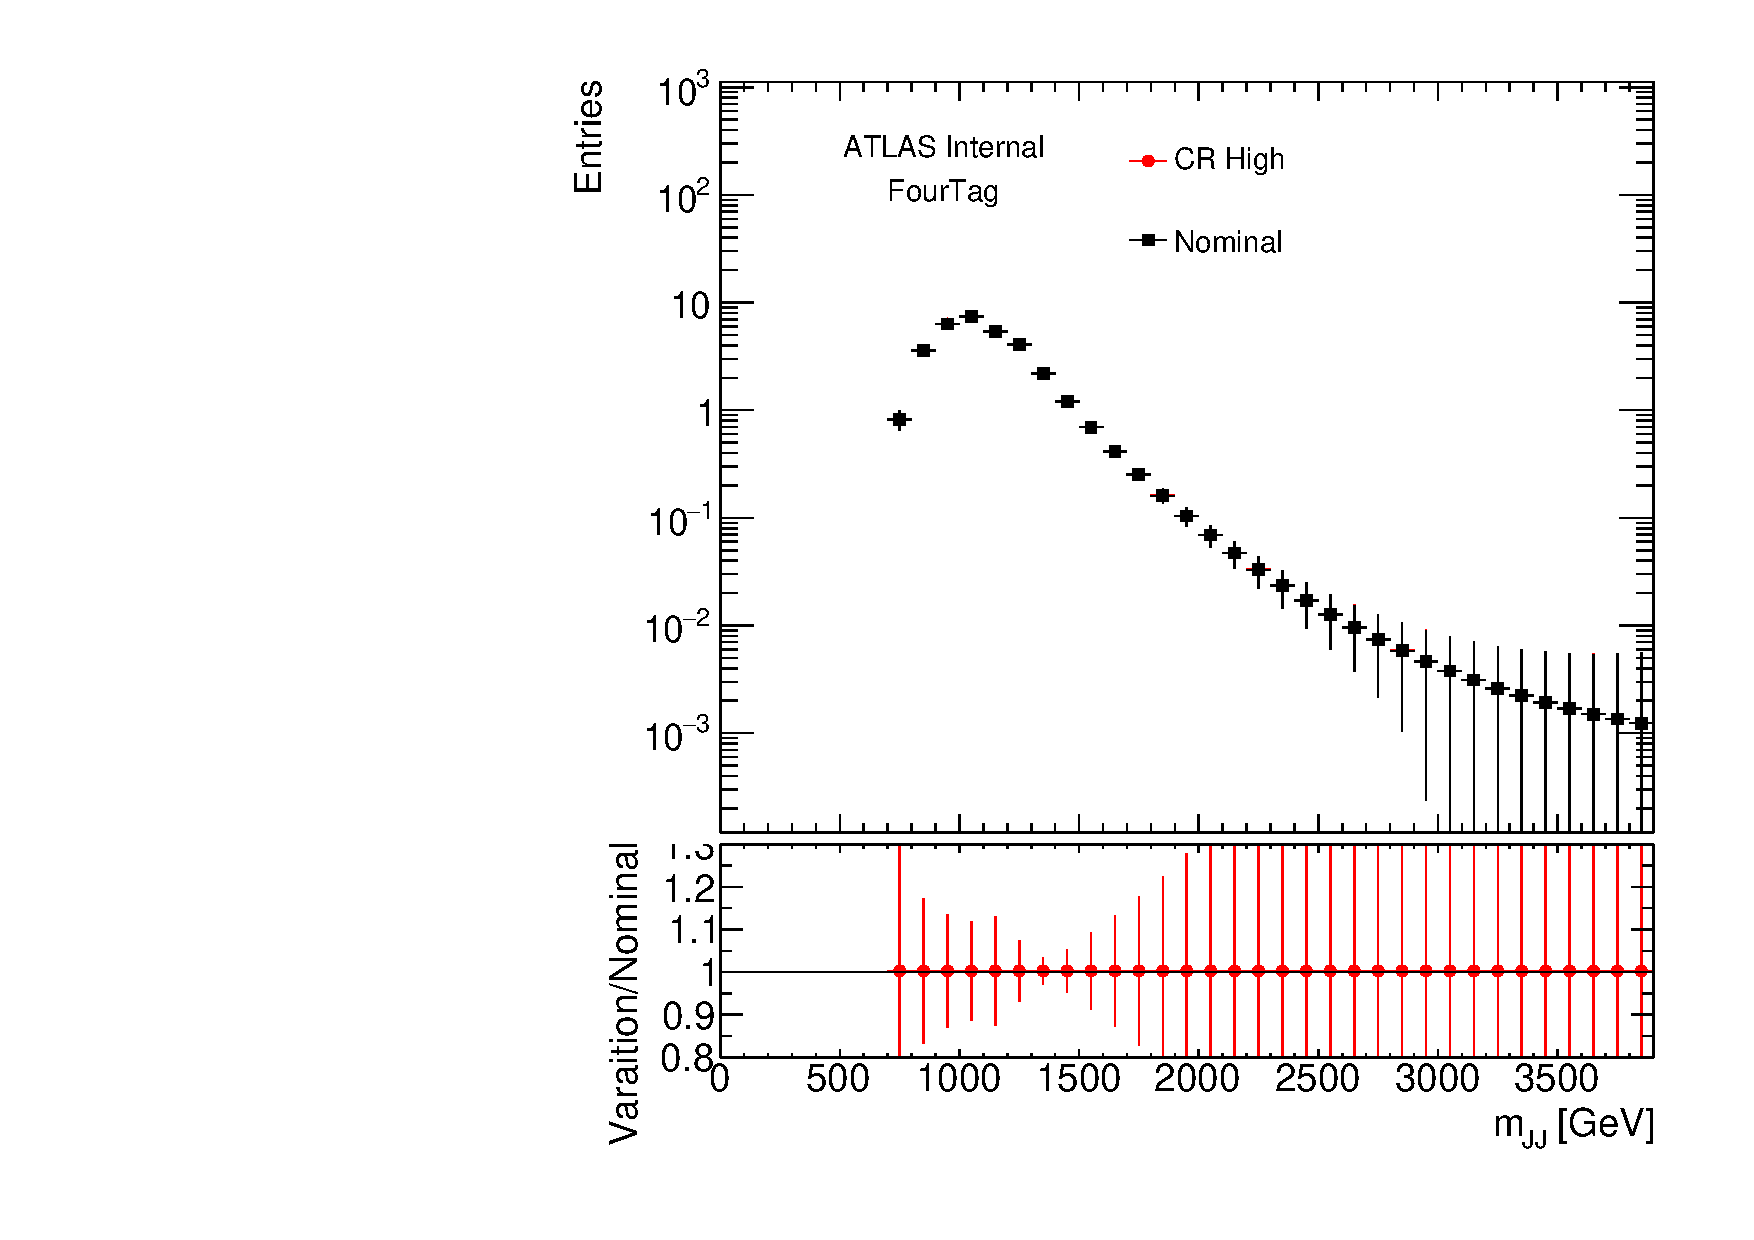
\includegraphics[width=0.31\textwidth,angle=-90]{figures/boosted/Syst_CRSB/CR_High_compare_FourTag_qcd_hh.pdf}
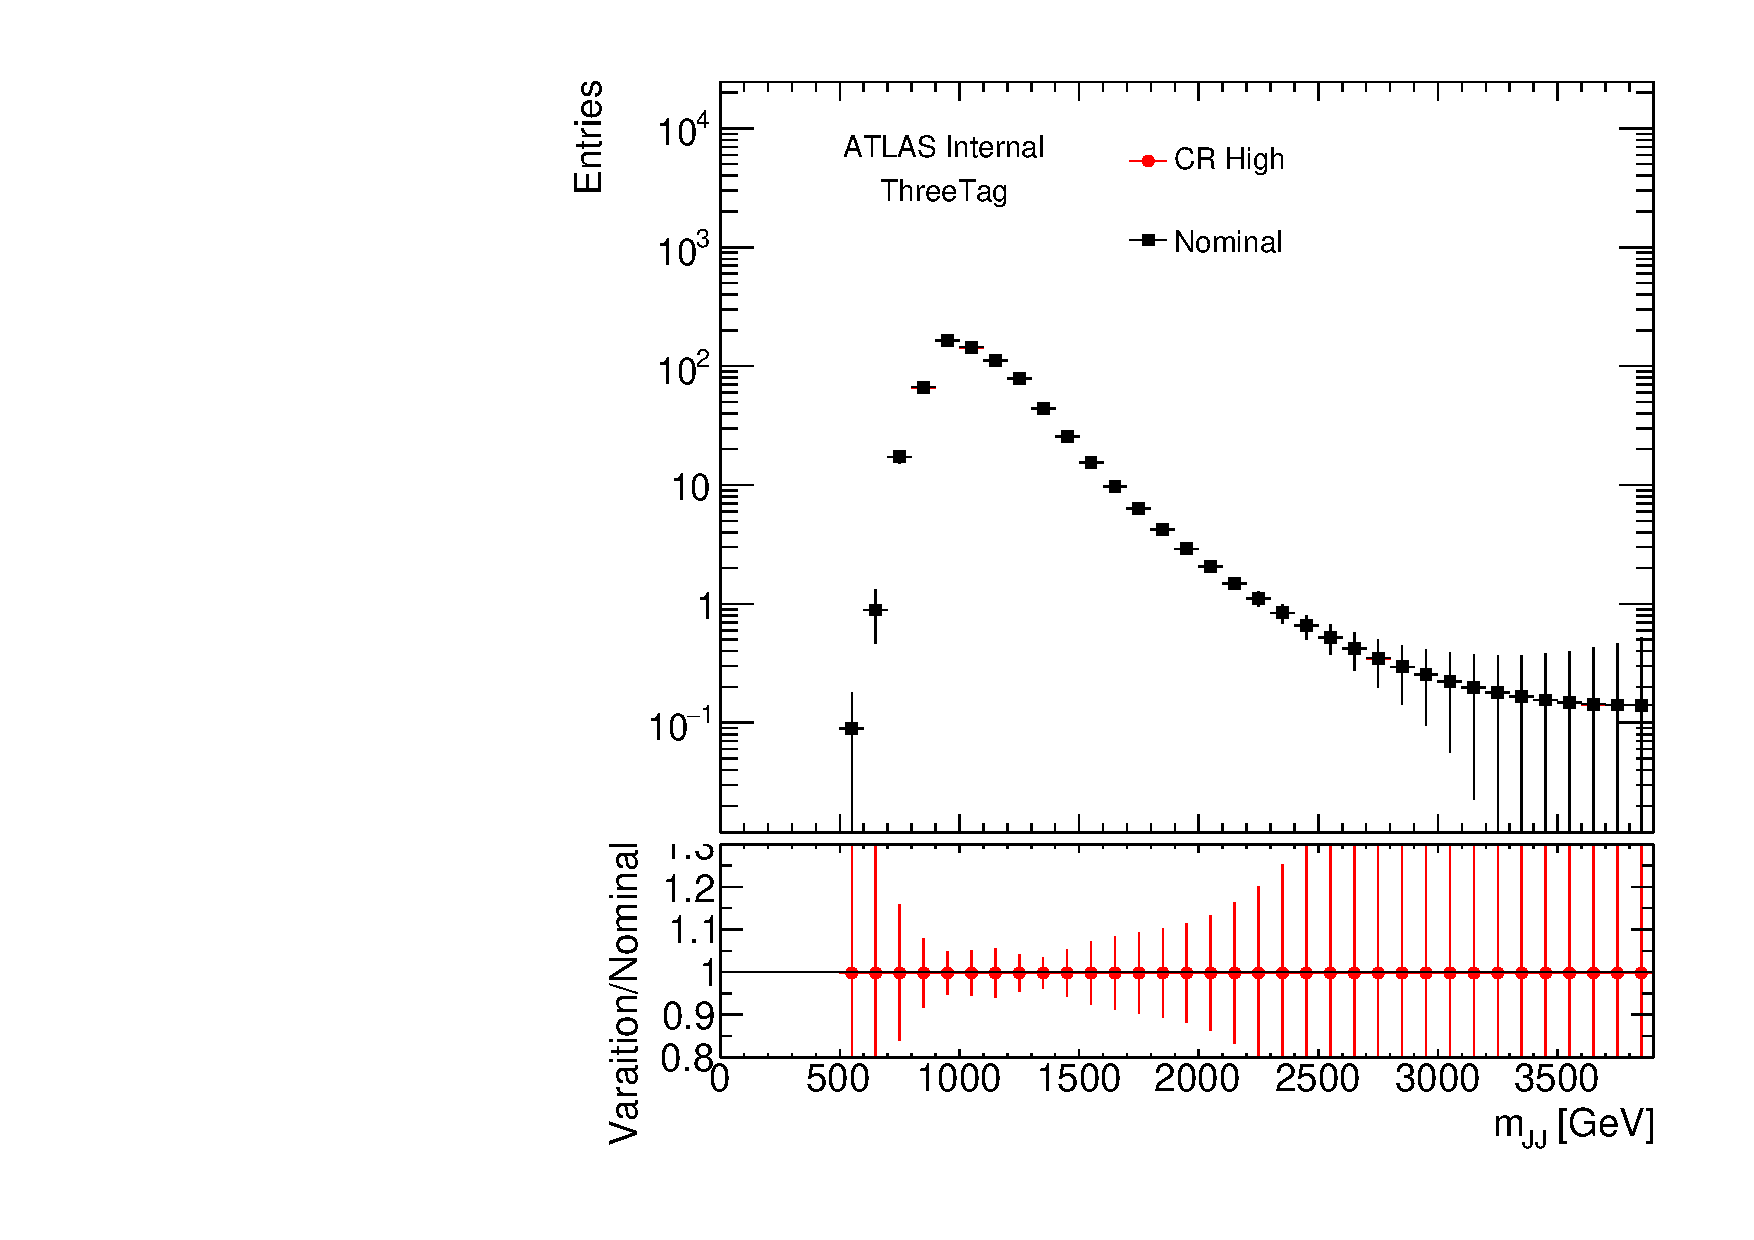
\includegraphics[width=0.31\textwidth,angle=-90]{figures/boosted/Syst_CRSB/CR_High_compare_ThreeTag_qcd_hh.pdf}
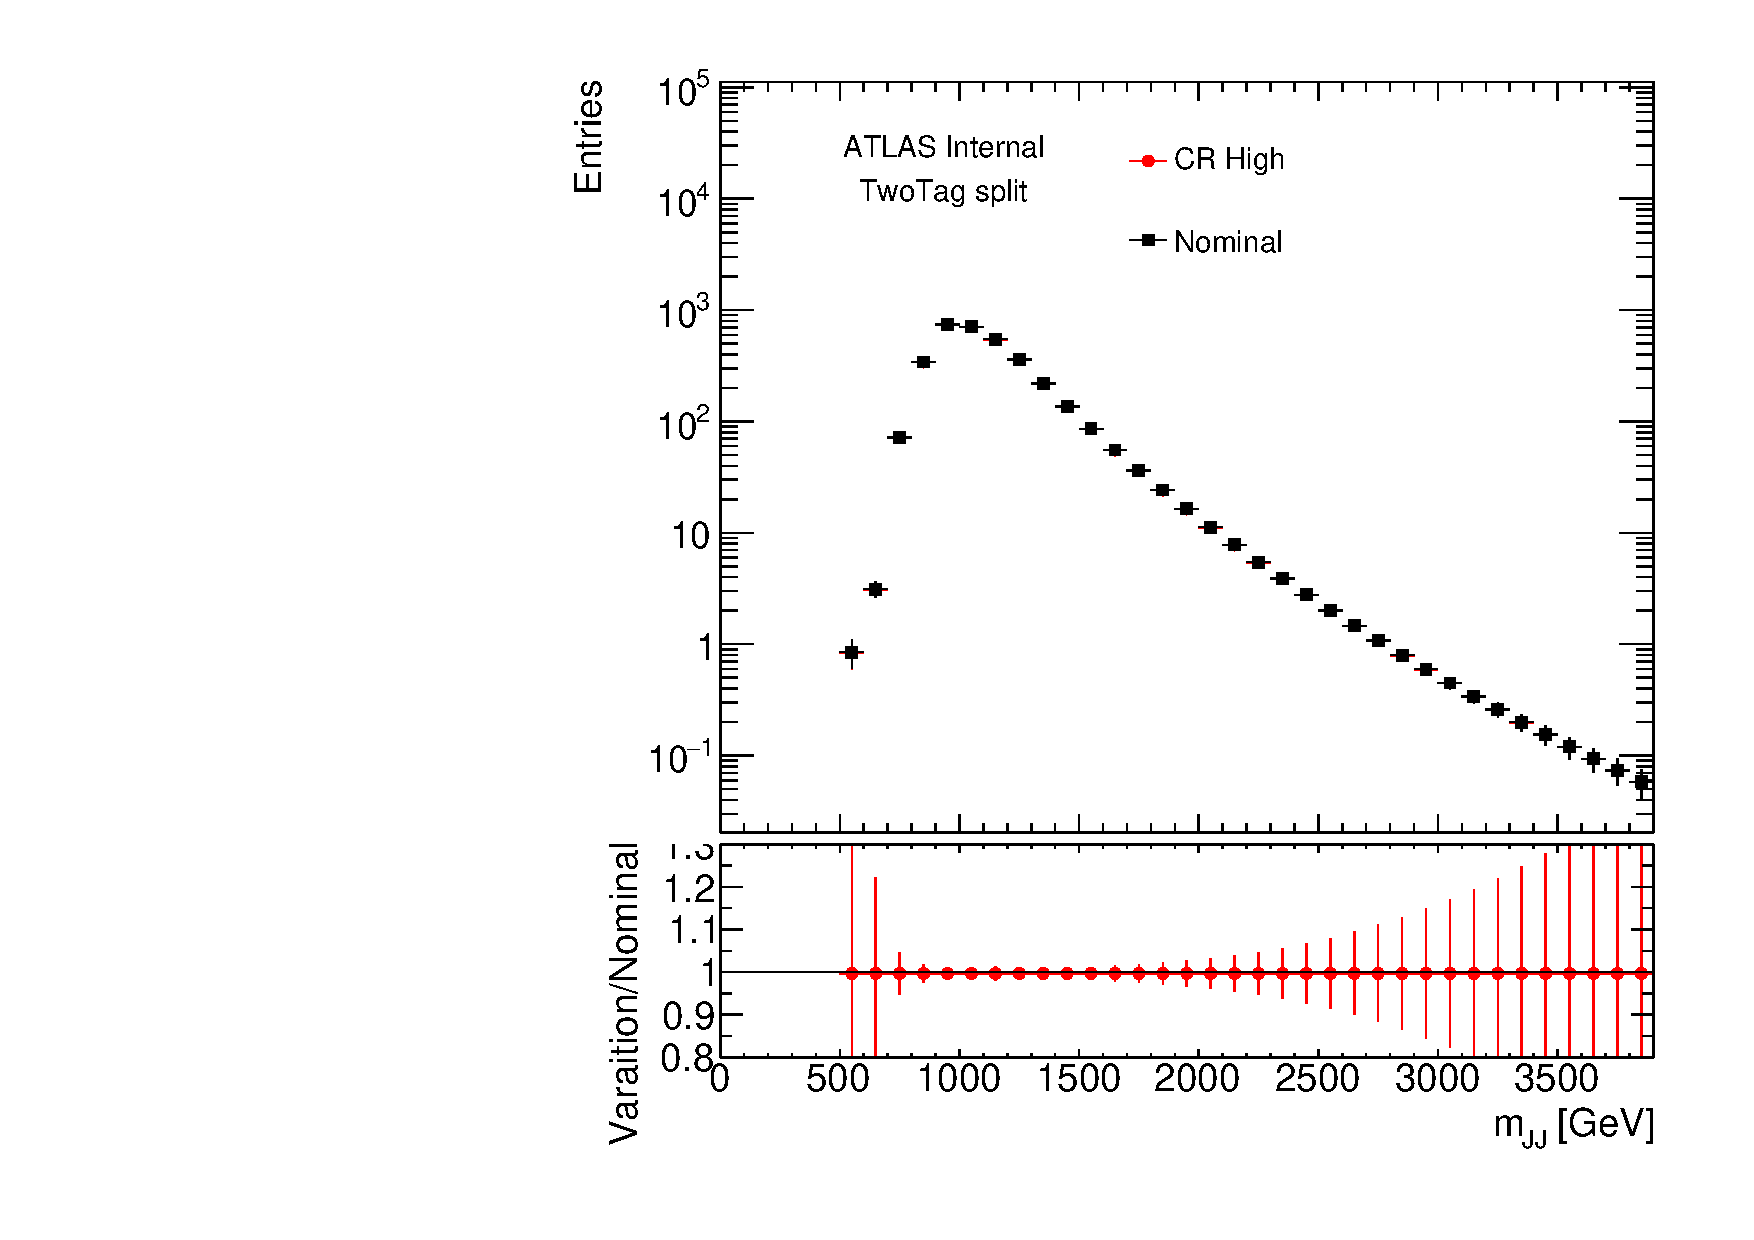
\includegraphics[width=0.31\textwidth,angle=-90]{figures/boosted/Syst_CRSB/CR_High_compare_TwoTag_split_qcd_hh.pdf}
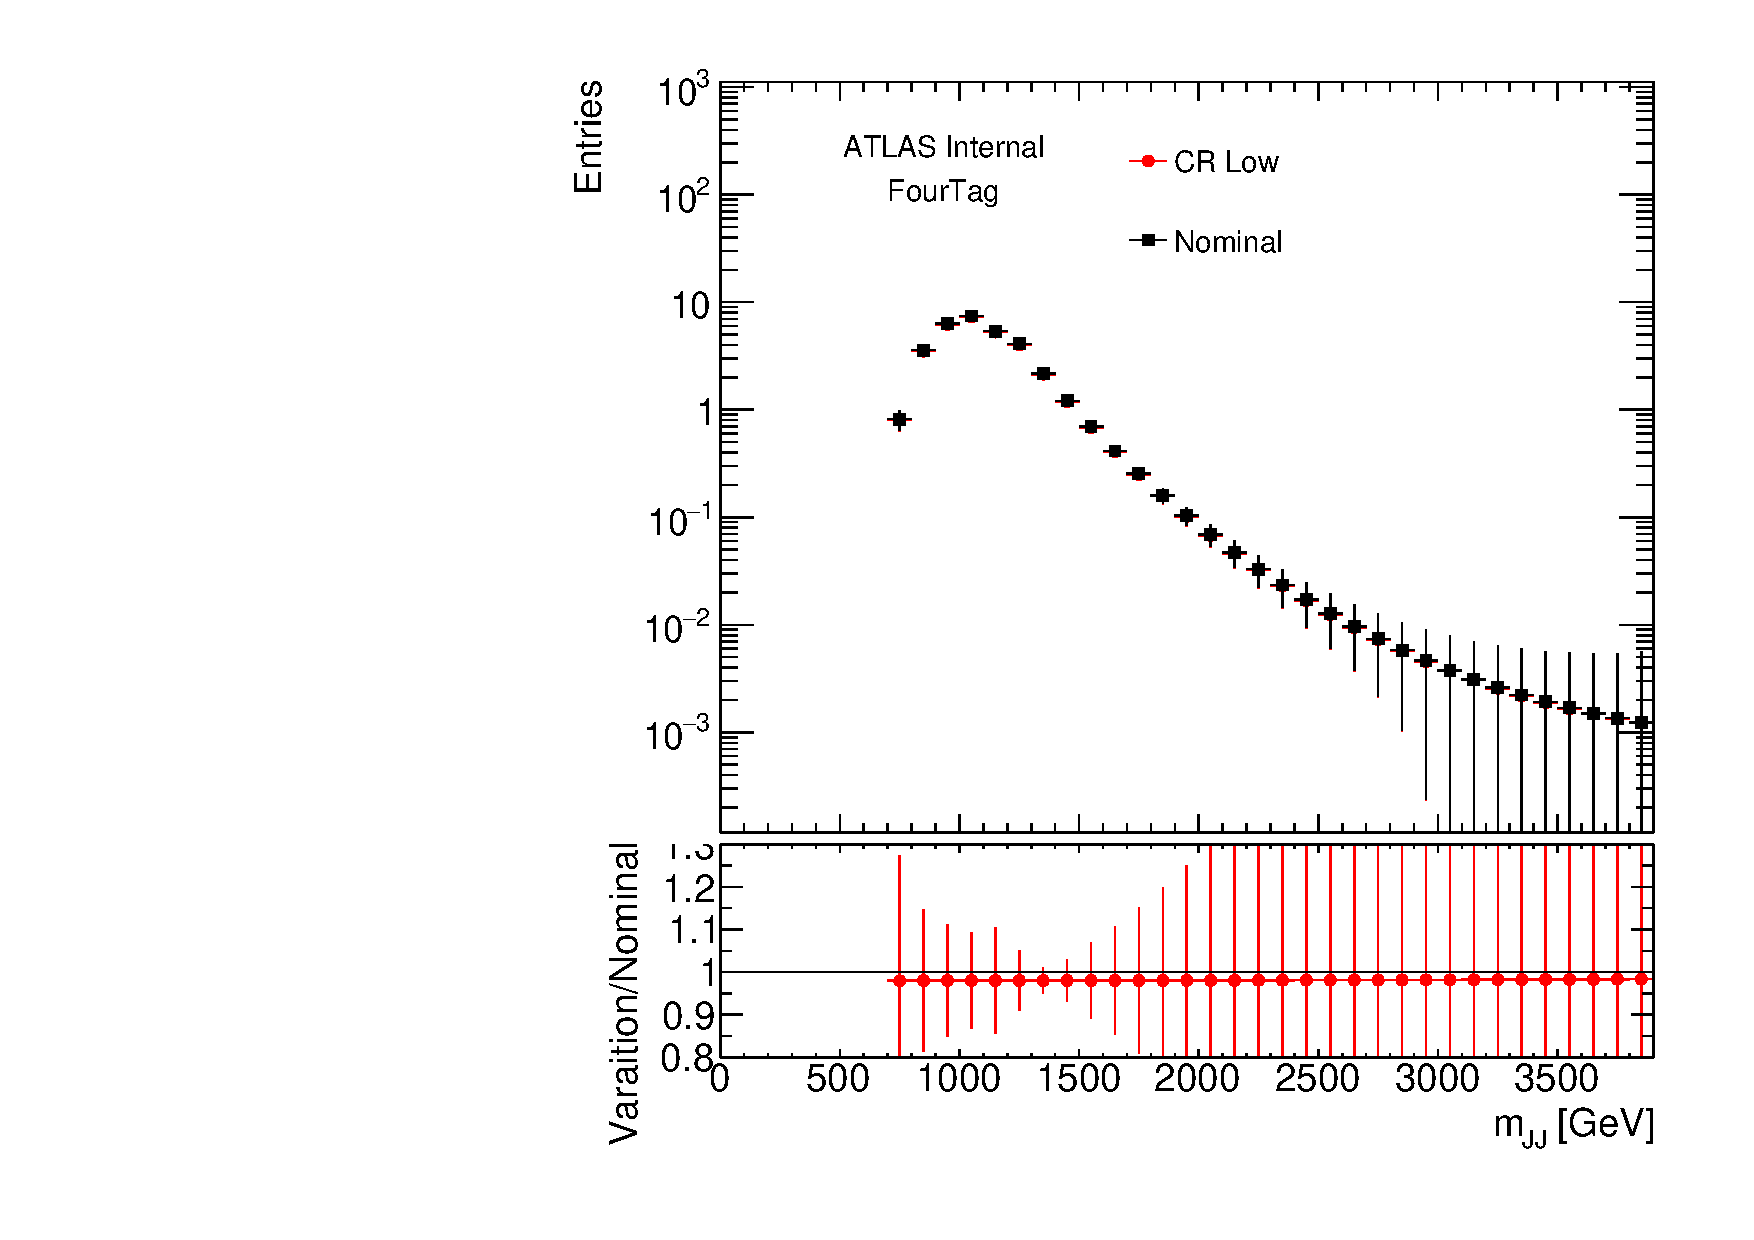
\includegraphics[width=0.31\textwidth,angle=-90]{figures/boosted/Syst_CRSB/CR_Low_compare_FourTag_qcd_hh.pdf}
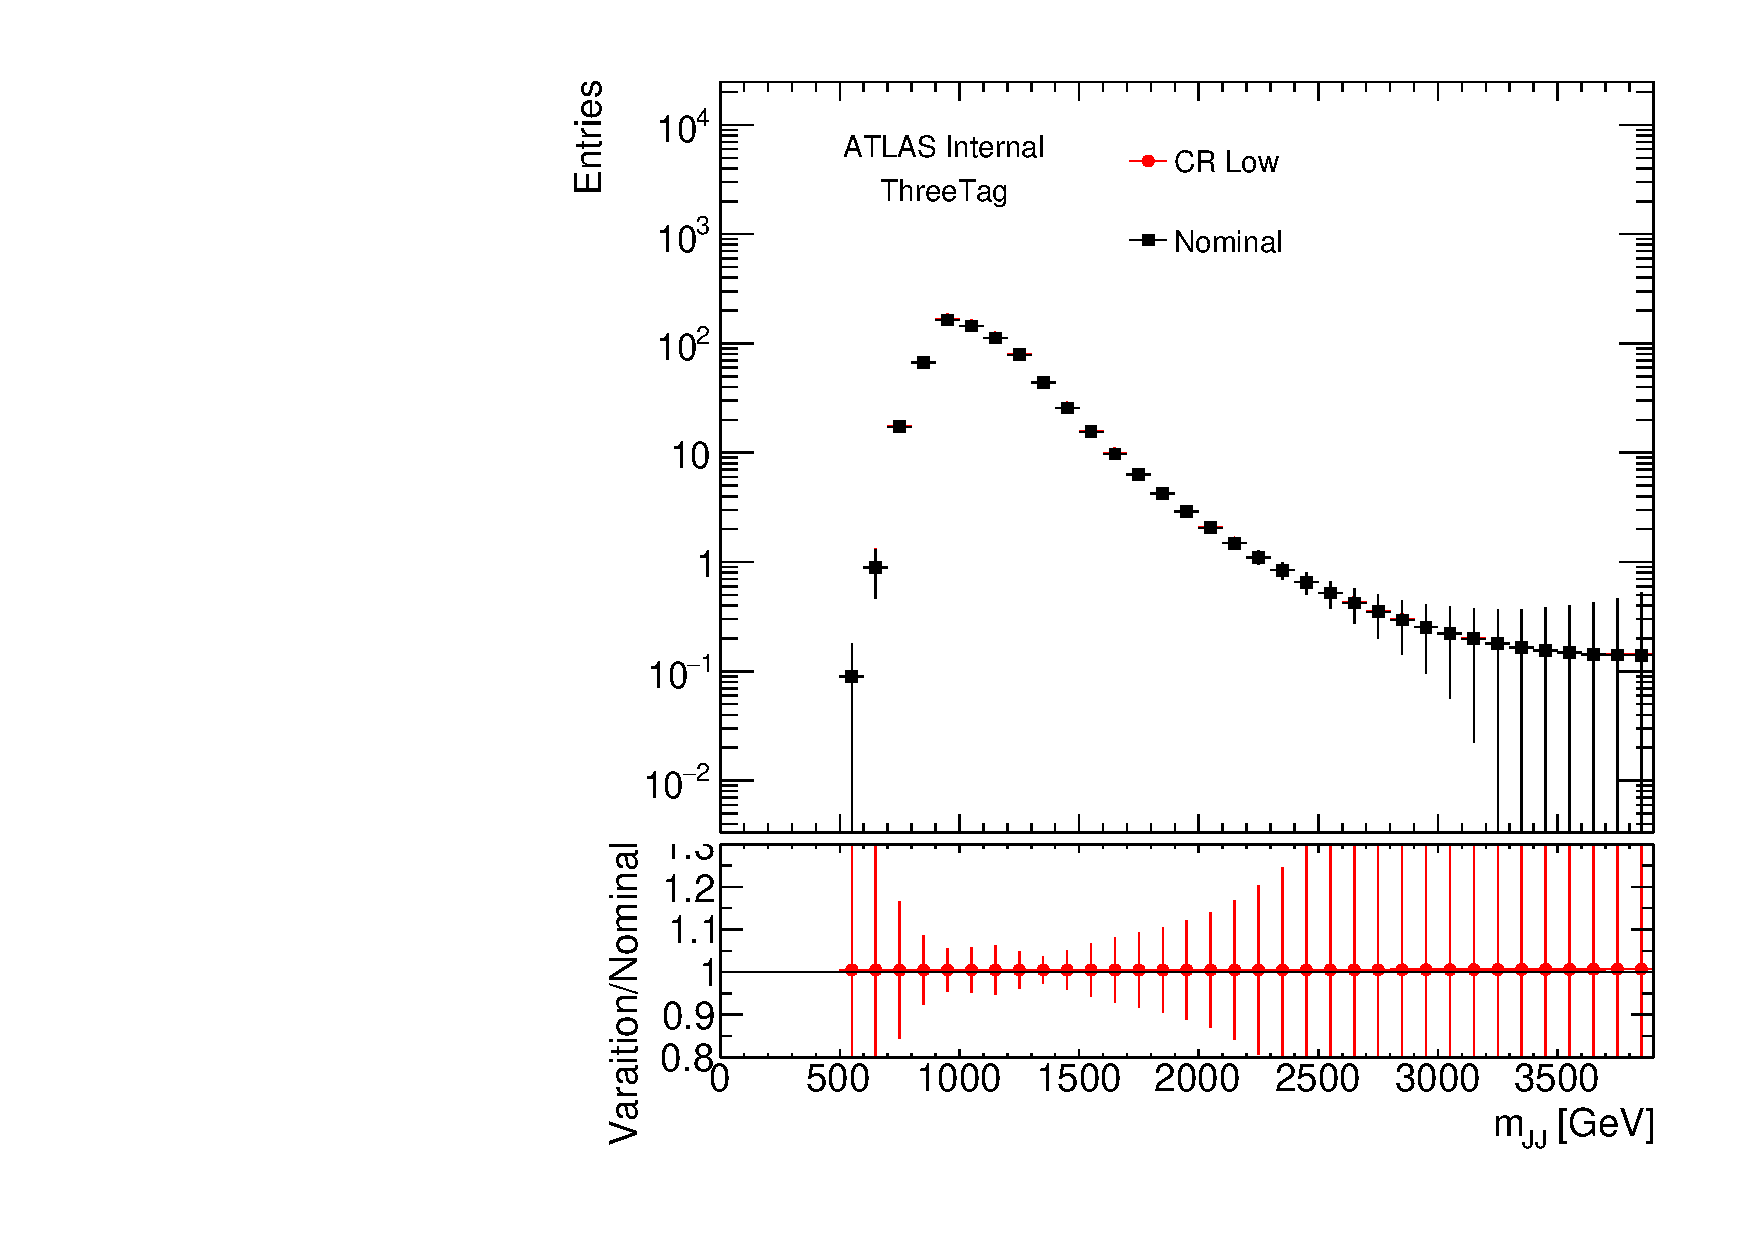
\includegraphics[width=0.31\textwidth,angle=-90]{figures/boosted/Syst_CRSB/CR_Low_compare_ThreeTag_qcd_hh.pdf}
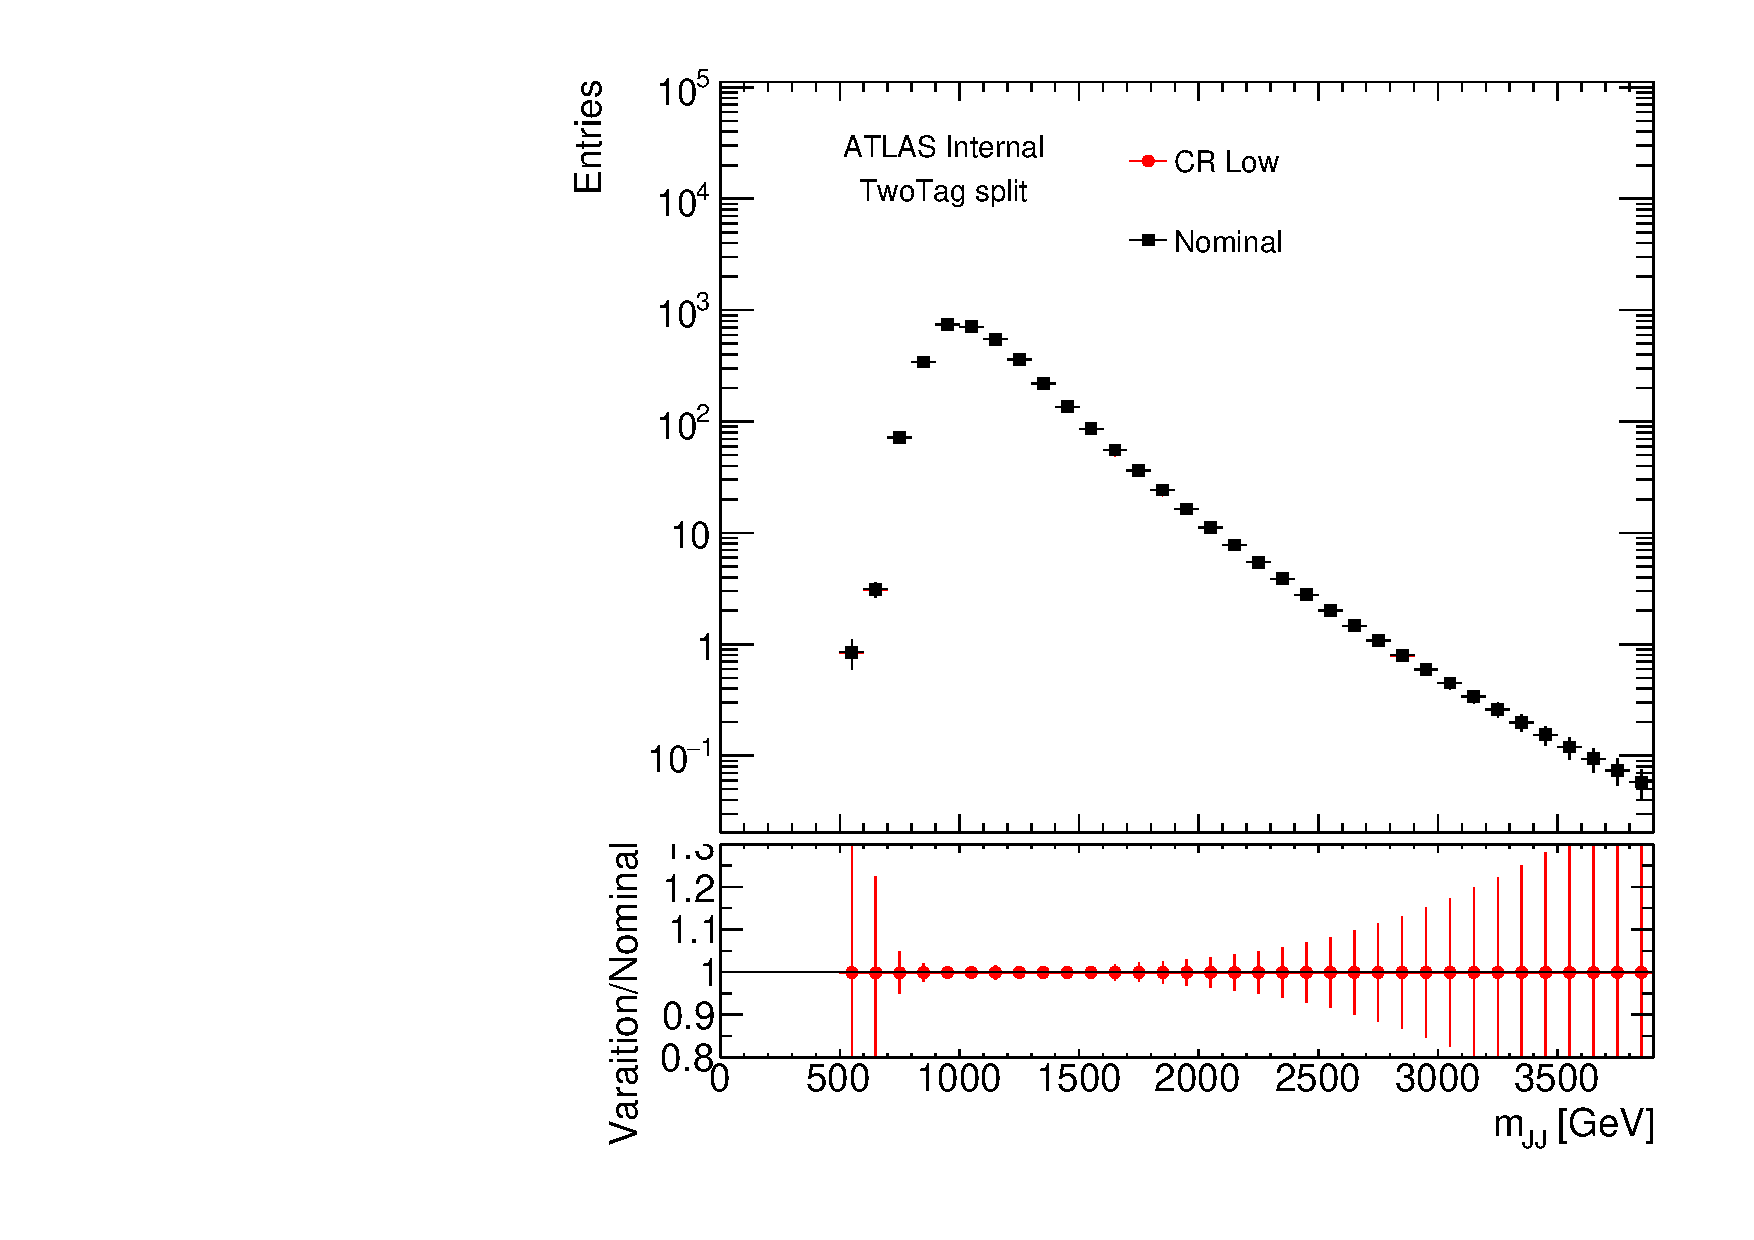
\includegraphics[width=0.31\textwidth,angle=-90]{figures/boosted/Syst_CRSB/CR_Low_compare_TwoTag_split_qcd_hh.pdf}
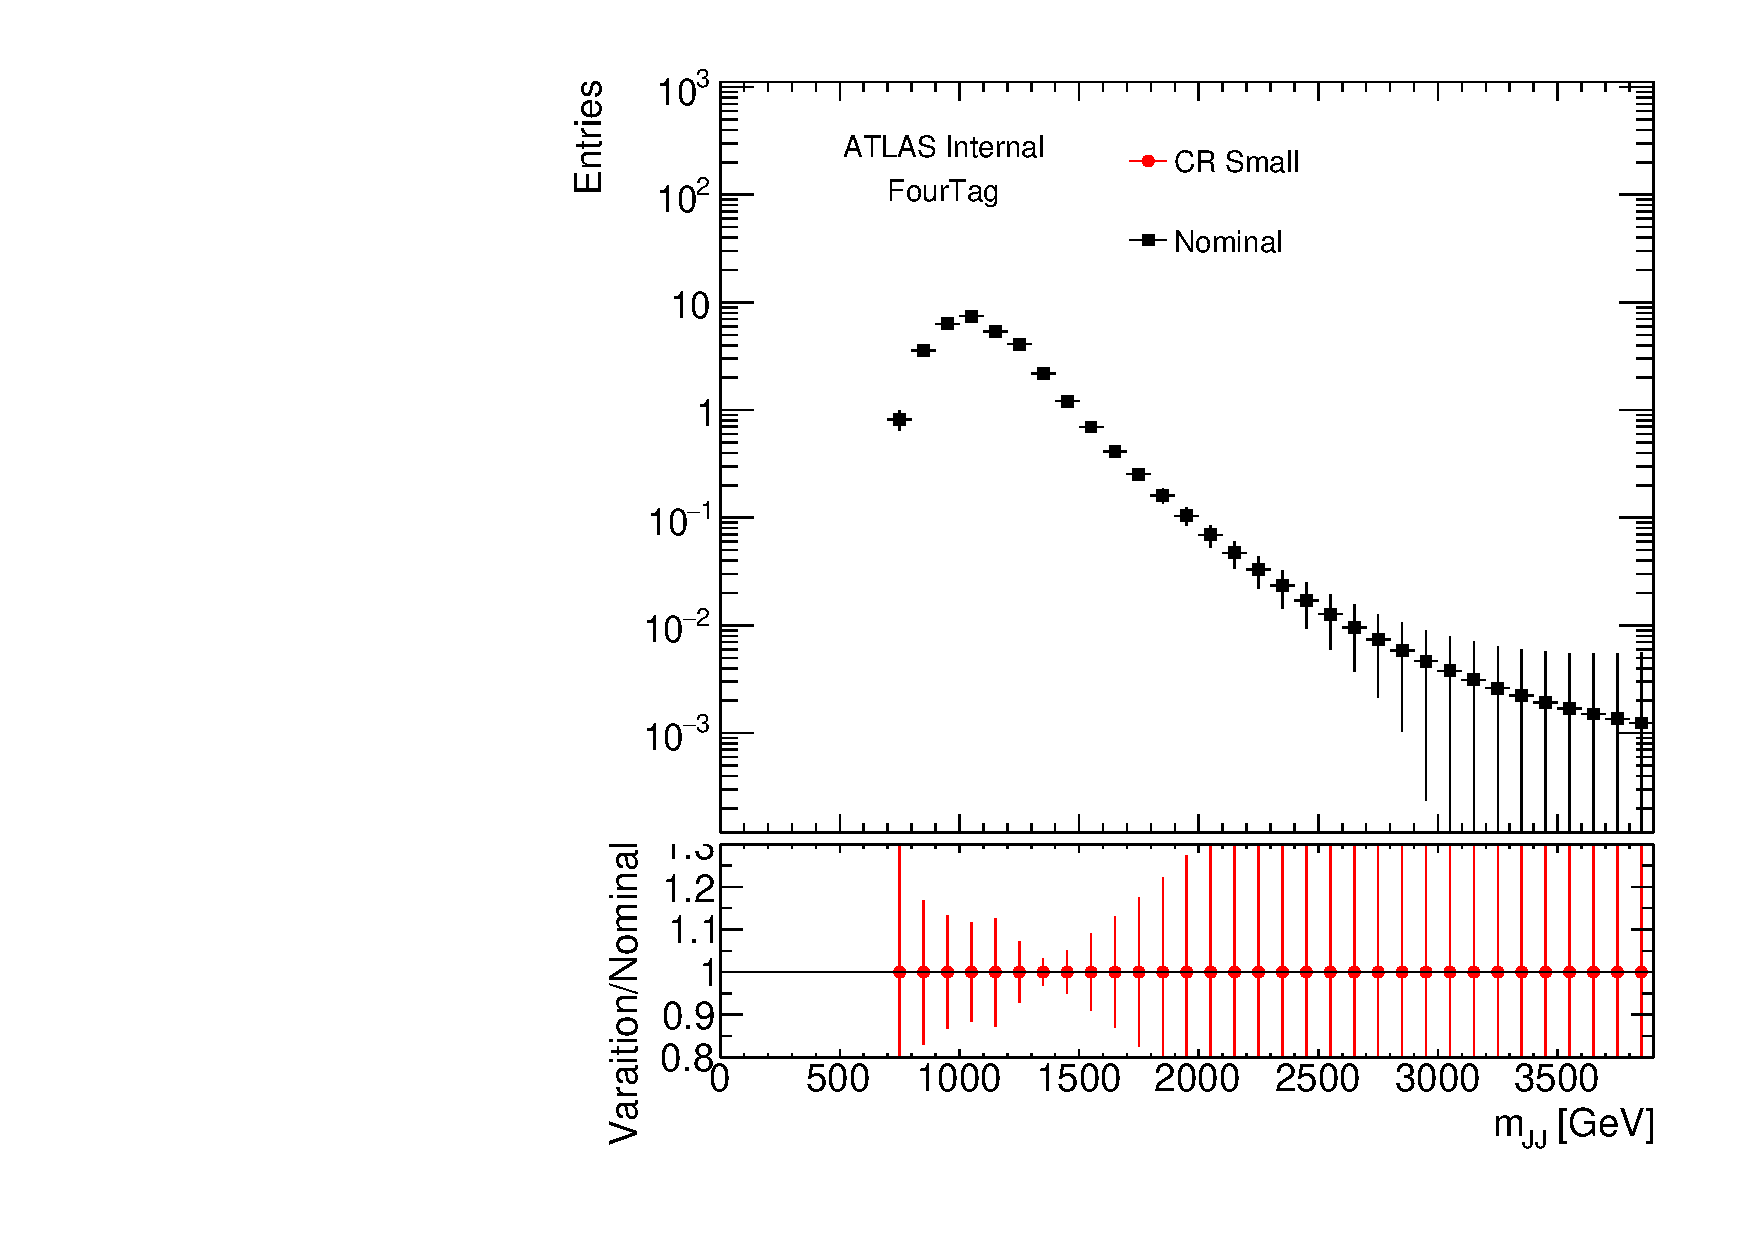
\includegraphics[width=0.31\textwidth,angle=-90]{figures/boosted/Syst_CRSB/CR_Small_compare_FourTag_qcd_hh.pdf}
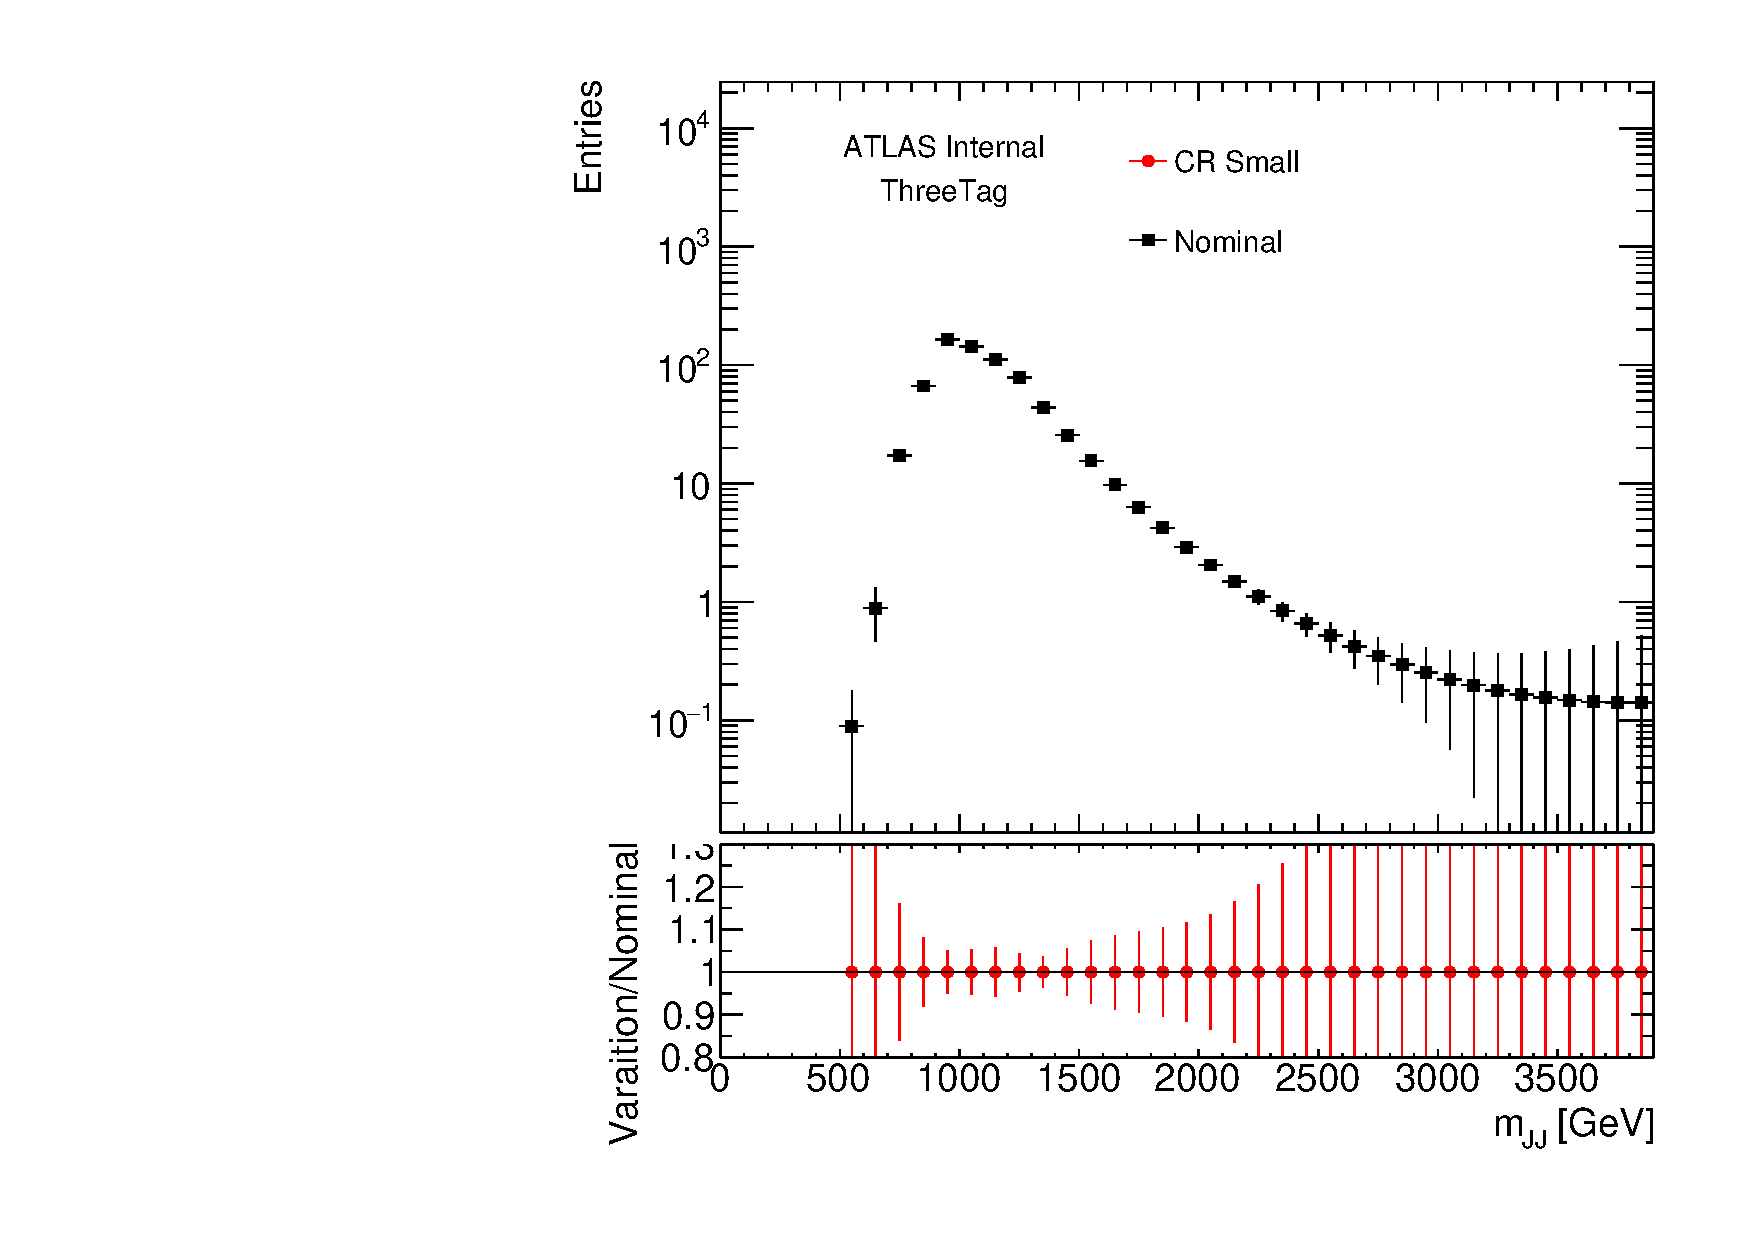
\includegraphics[width=0.31\textwidth,angle=-90]{figures/boosted/Syst_CRSB/CR_Small_compare_ThreeTag_qcd_hh.pdf}
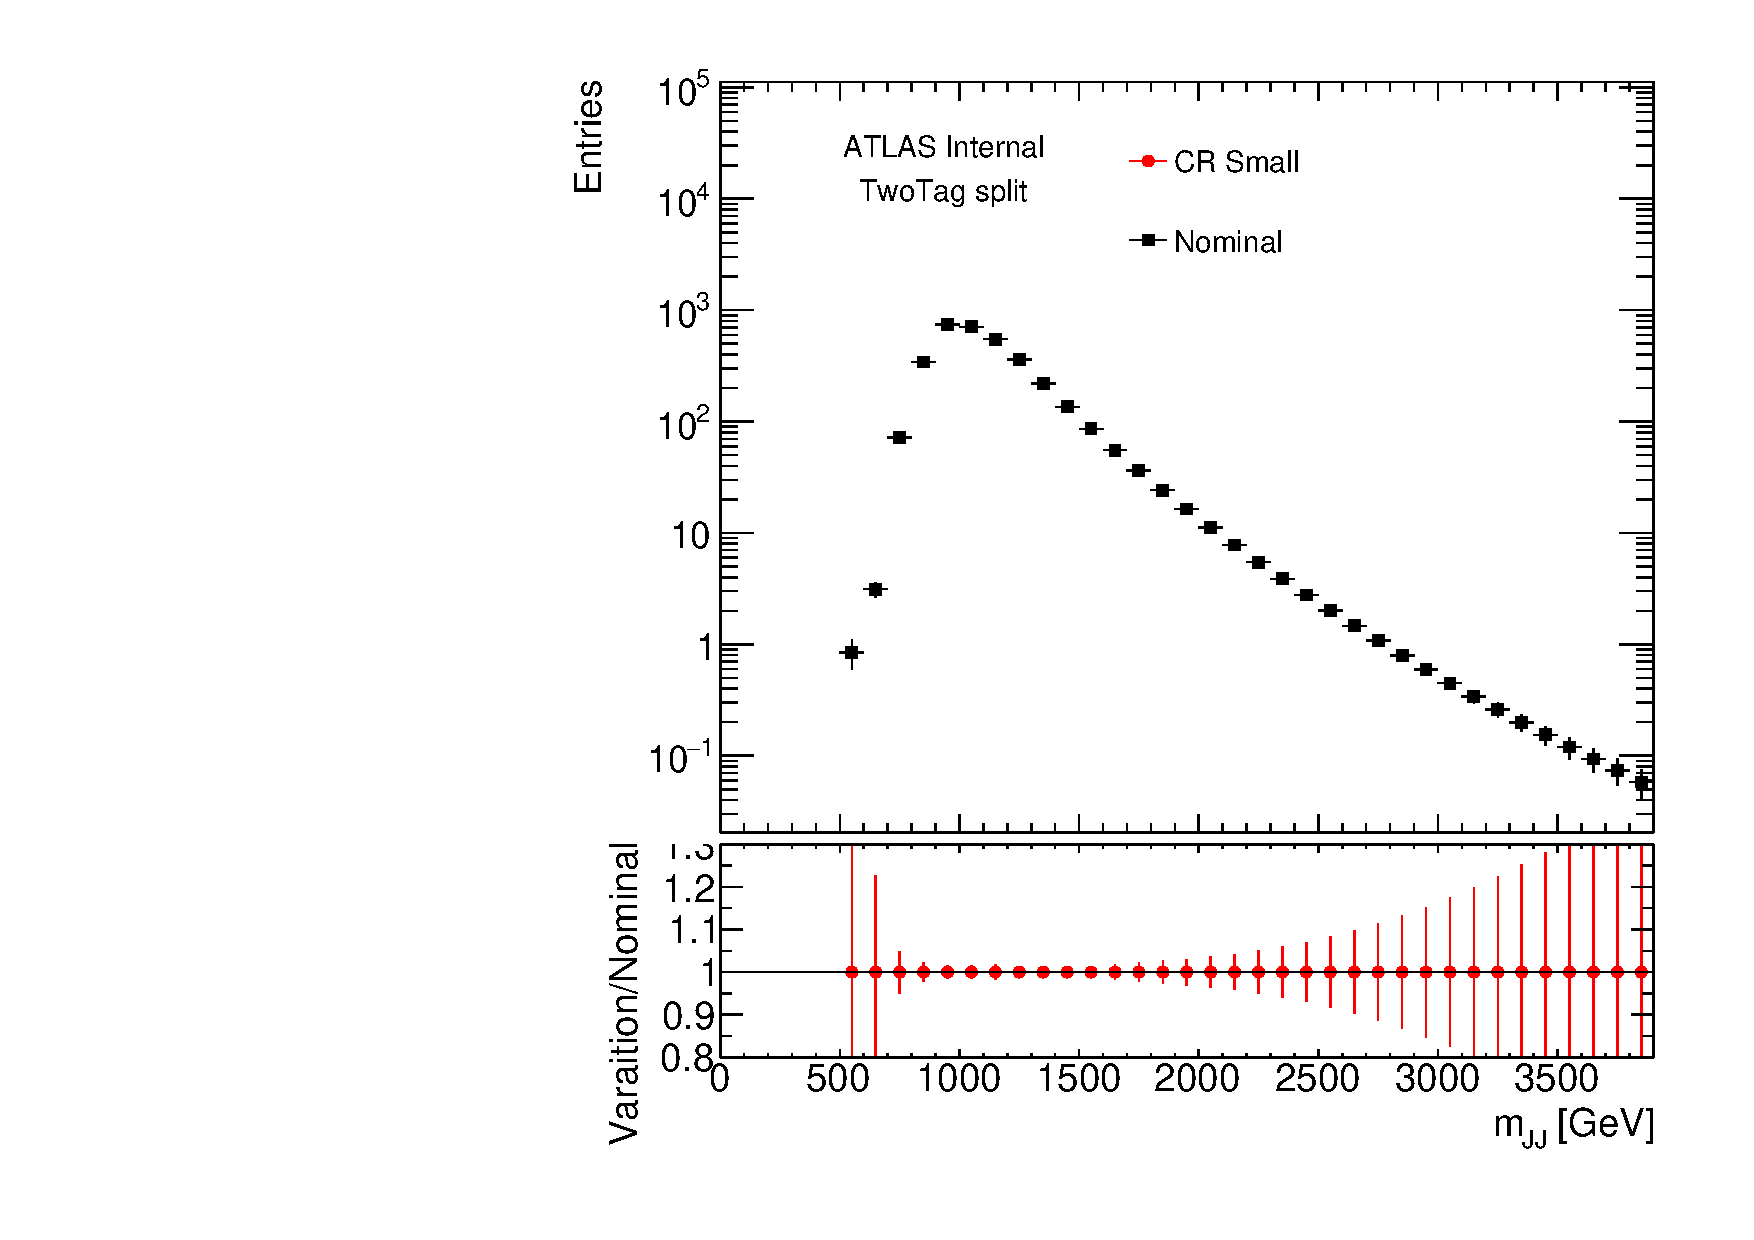
\includegraphics[width=0.31\textwidth,angle=-90]{figures/boosted/Syst_CRSB/CR_Small_compare_TwoTag_split_qcd_hh.pdf}
\end{center}
\caption{Comparisons of the nominal QCD shape prediction (black) with the results of control and sideband region variations (red). The ratio of the shape from each variation to the nominal shape is shown in the lower panel. The left column shows the relevant distributions for the $4b$ signal region, the middle column is for the $3b$ signal region, and the left column is for the $2bs$ signal region. The top row is for the high CR variation, the middle row is for the low CR variation, and the bottom row is for the small CR variation.}
\label{CRSB:QCDShapeSR-CR}
\end{figure}

\begin{figure}[htbp!]
\begin{center}
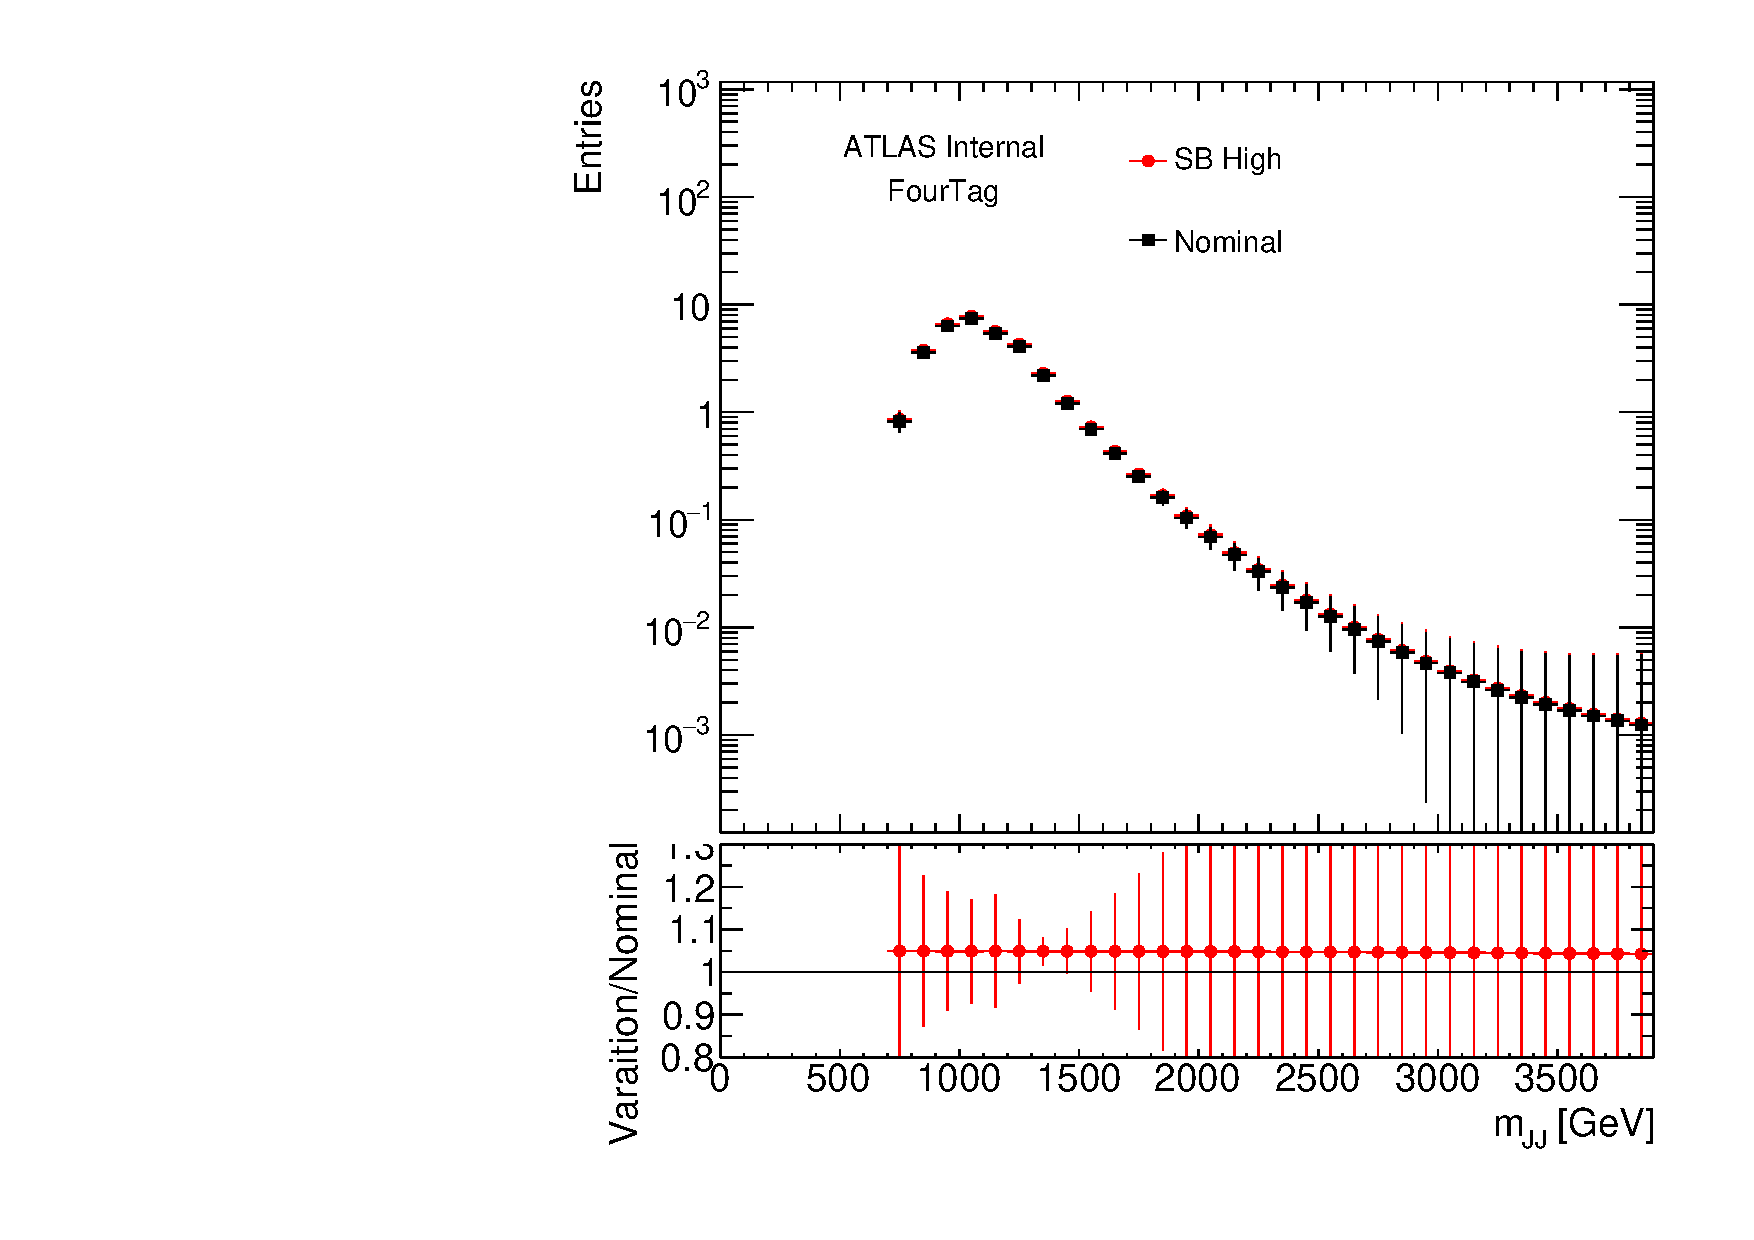
\includegraphics[width=0.25\textwidth,angle=-90]{figures/boosted/Syst_CRSB/SB_High_compare_FourTag_qcd_hh.pdf}
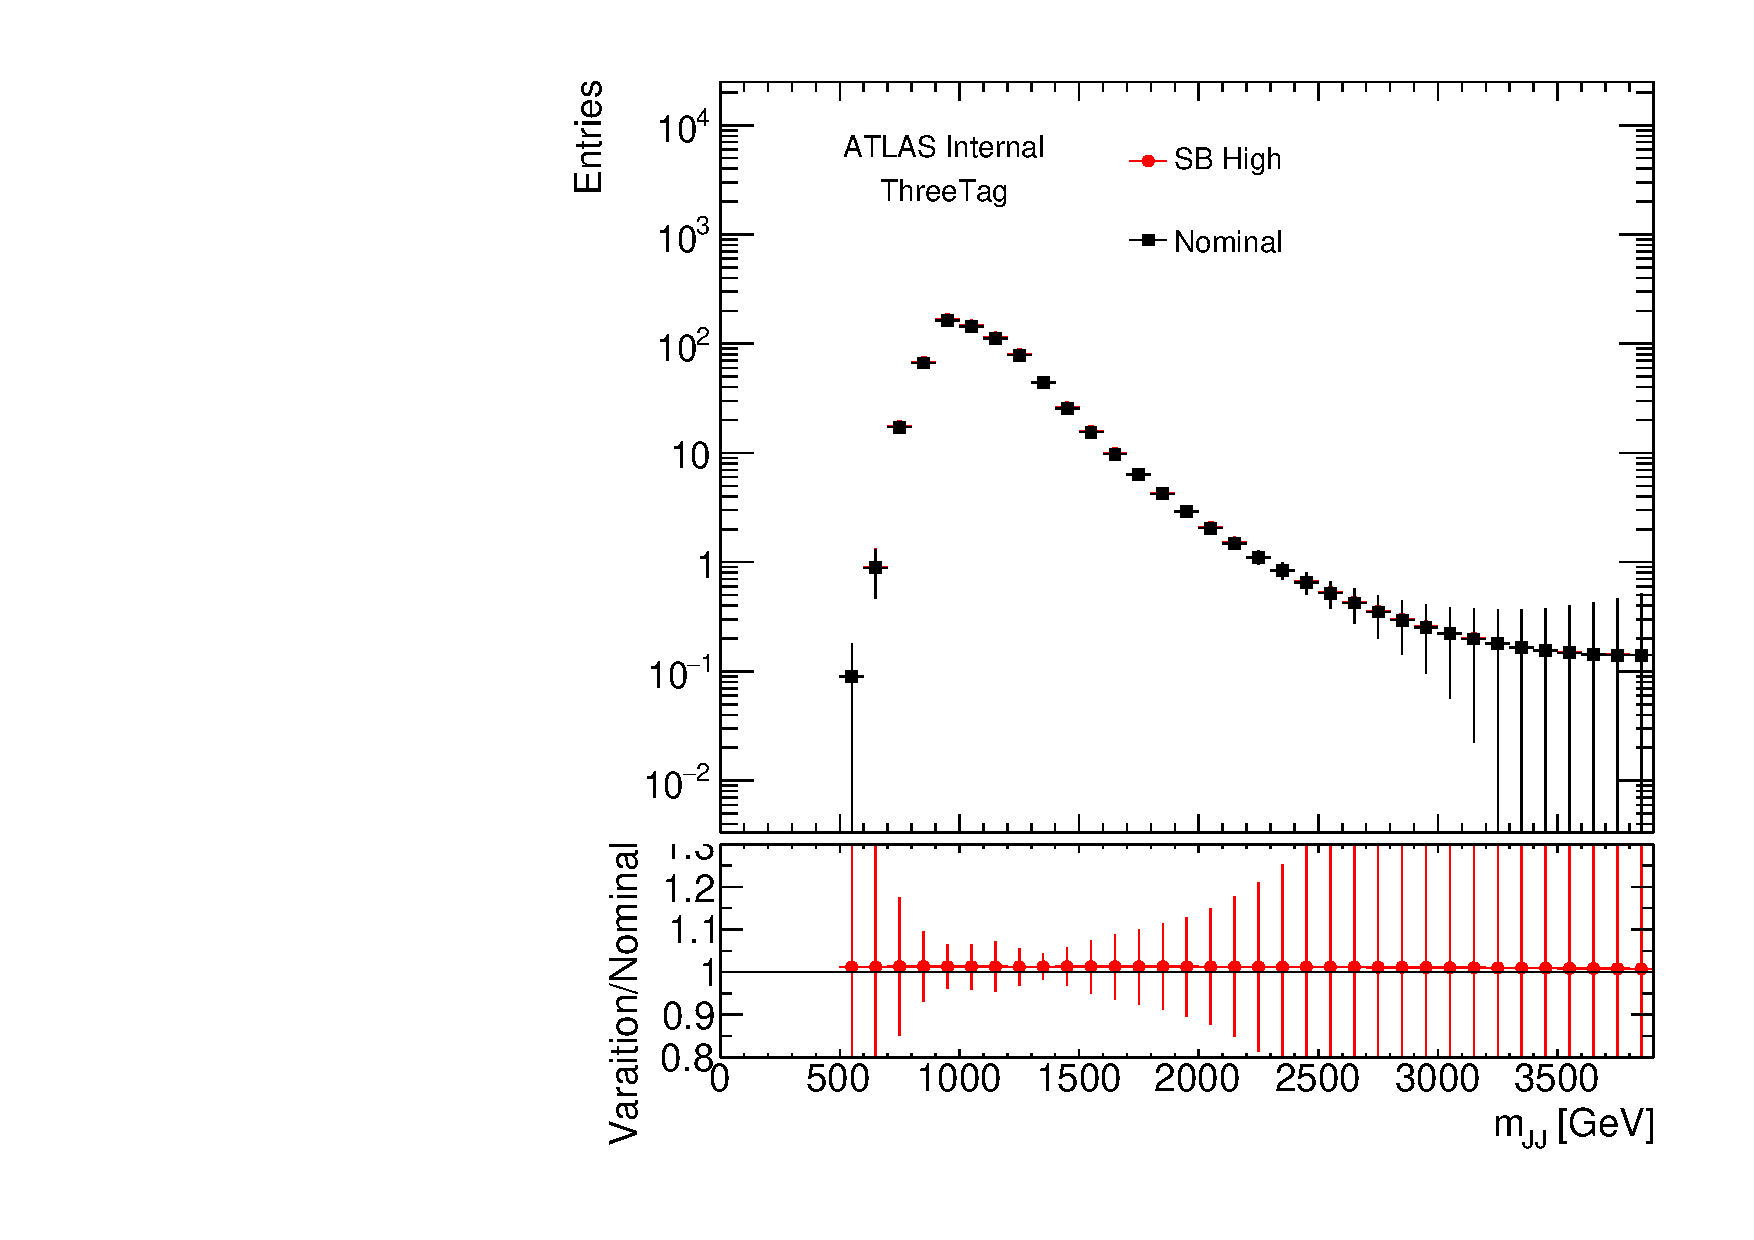
\includegraphics[width=0.25\textwidth,angle=-90]{figures/boosted/Syst_CRSB/SB_High_compare_ThreeTag_qcd_hh.pdf}
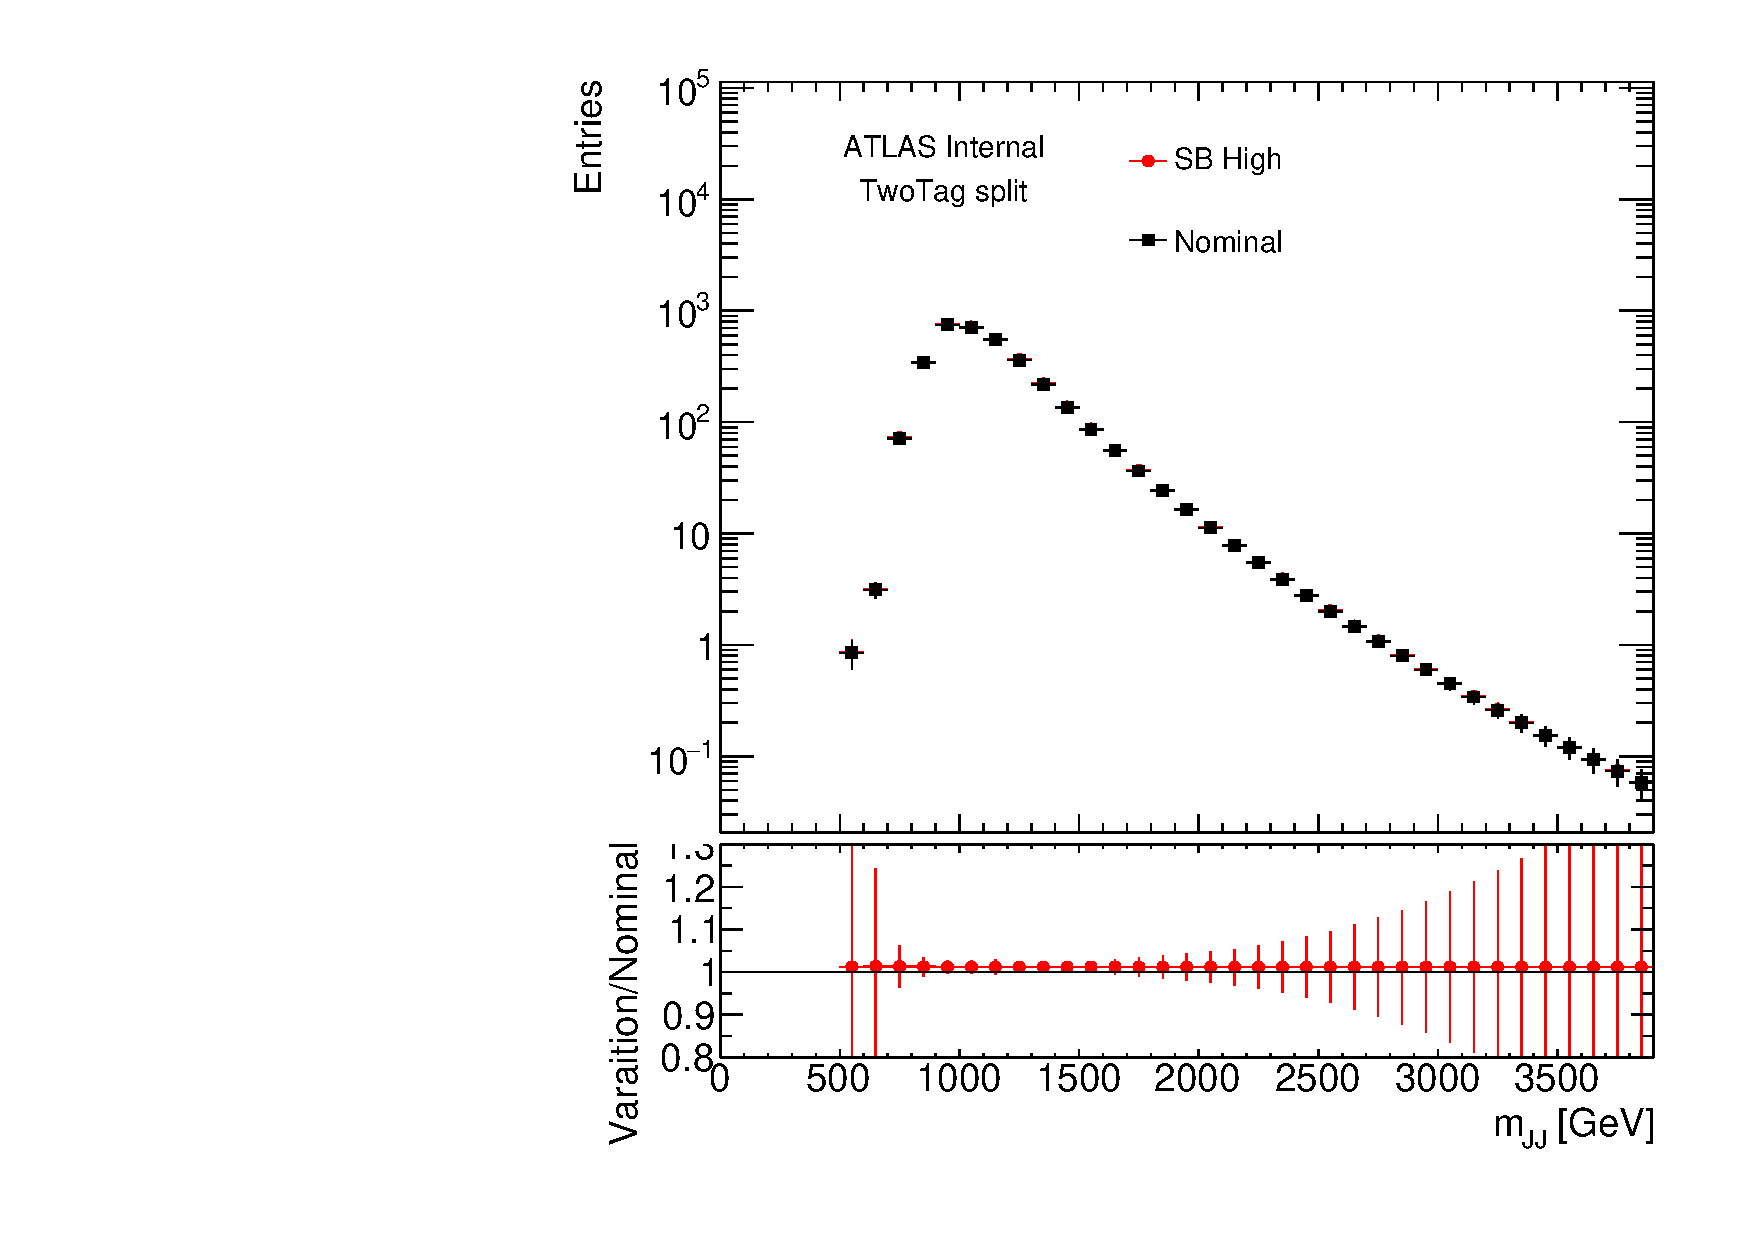
\includegraphics[width=0.25\textwidth,angle=-90]{figures/boosted/Syst_CRSB/SB_High_compare_TwoTag_split_qcd_hh.pdf}
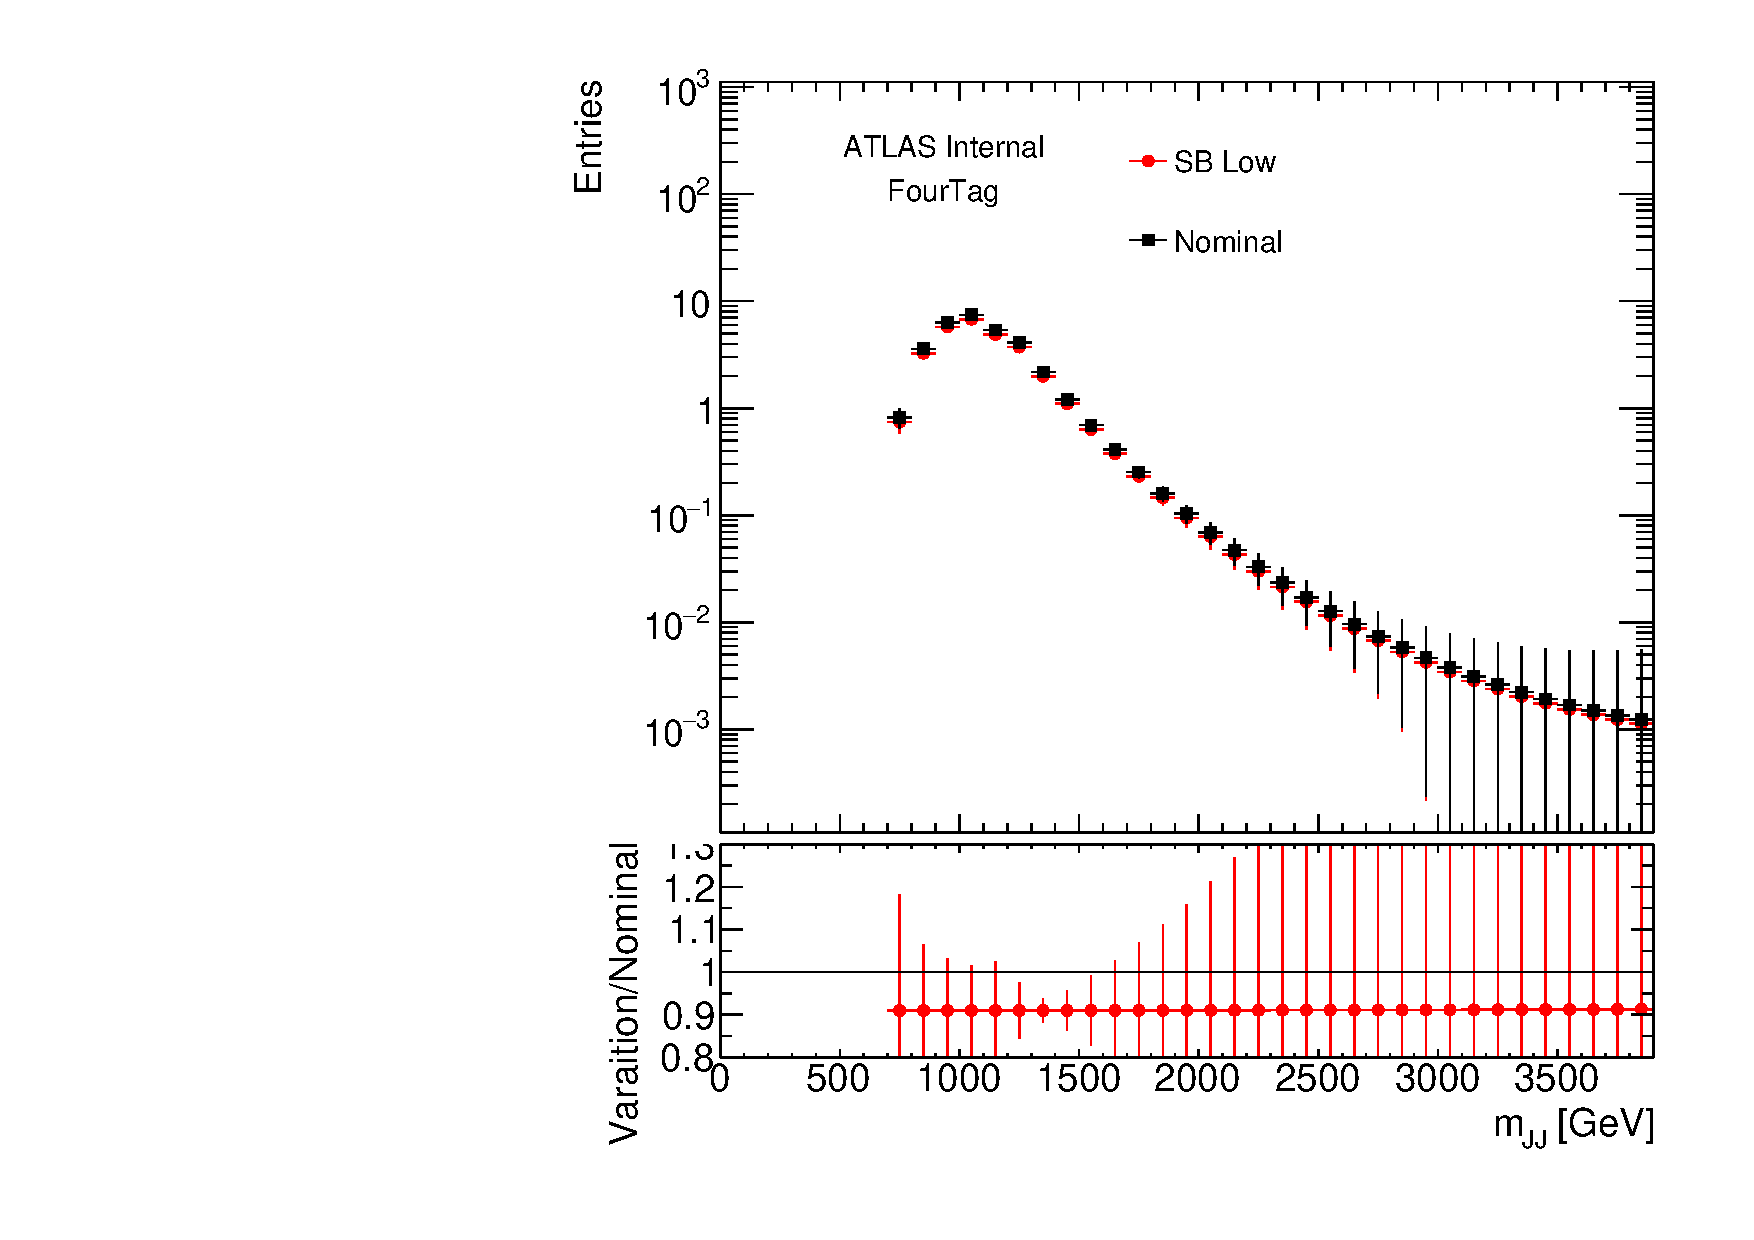
\includegraphics[width=0.25\textwidth,angle=-90]{figures/boosted/Syst_CRSB/SB_Low_compare_FourTag_qcd_hh.pdf}
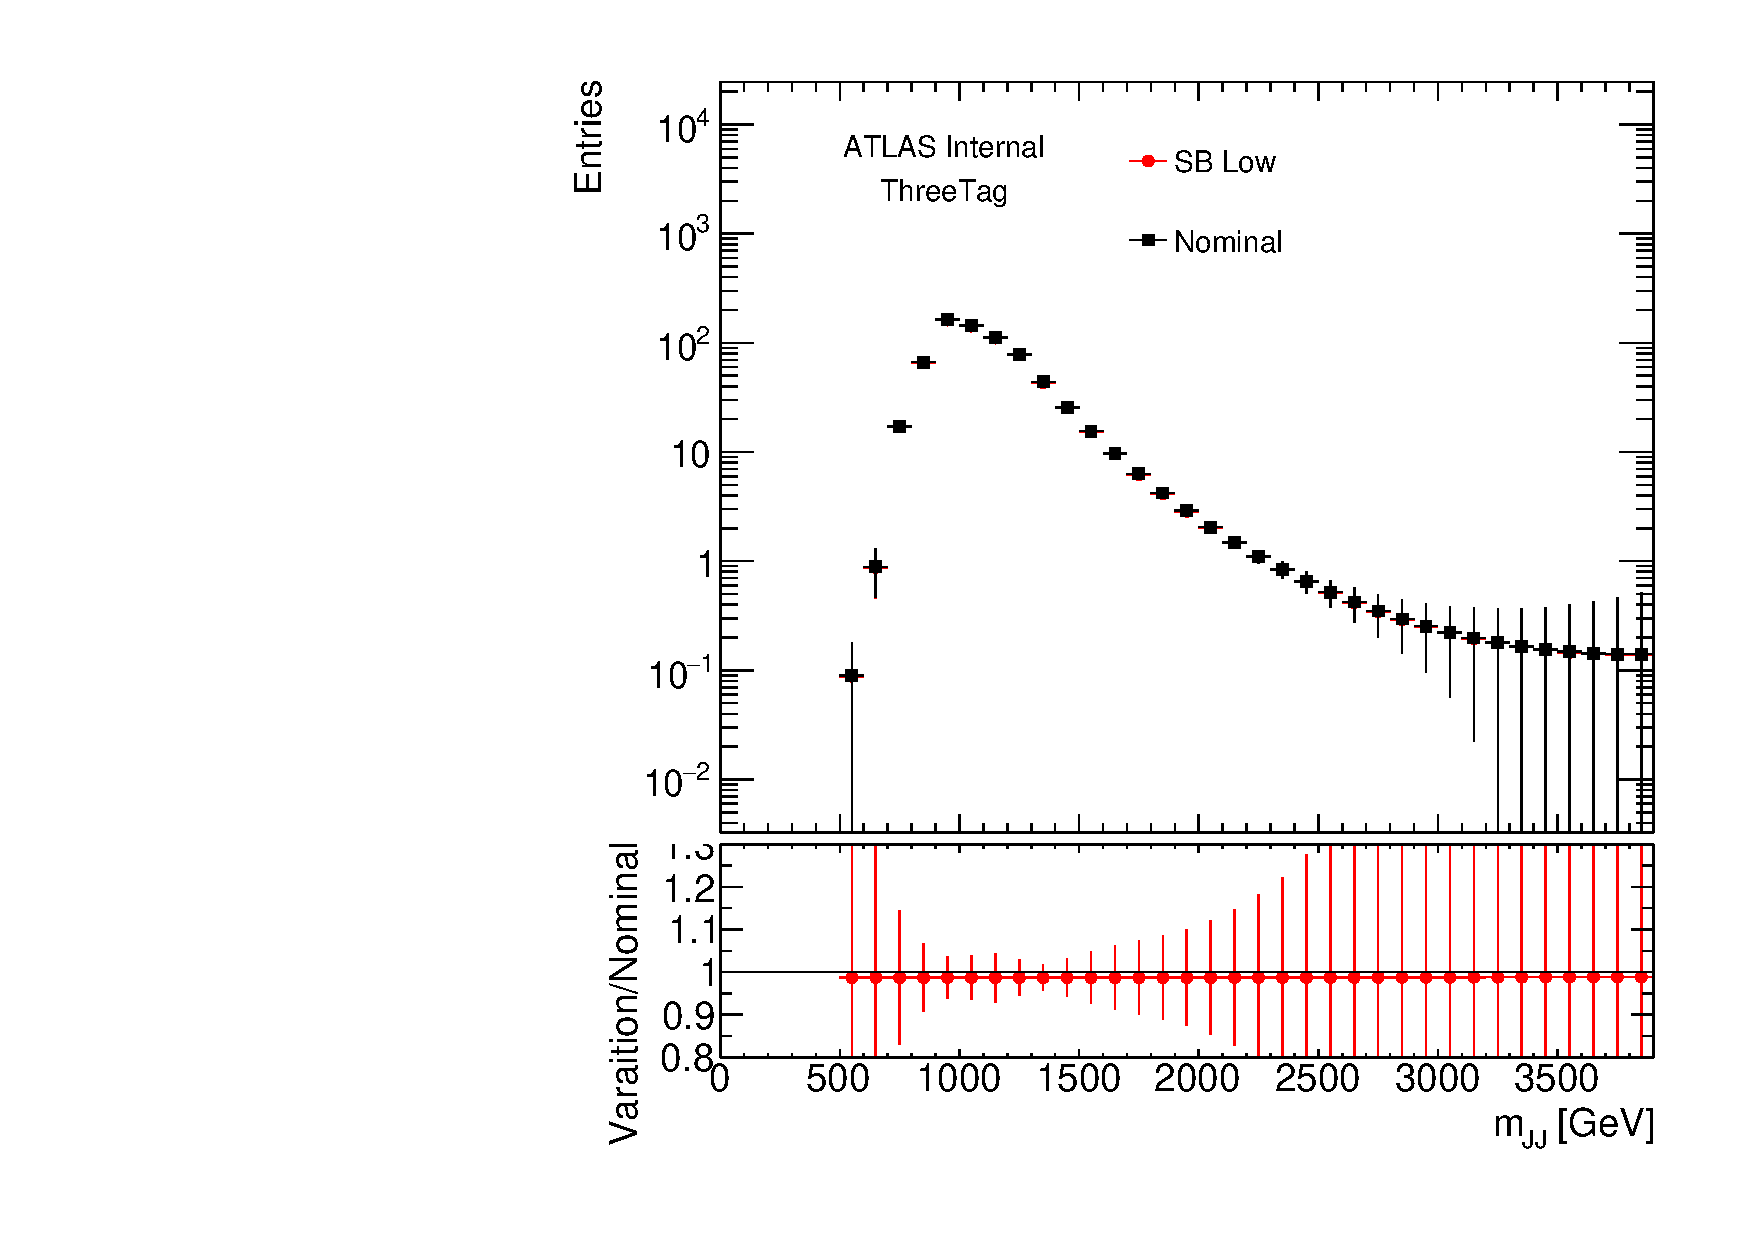
\includegraphics[width=0.25\textwidth,angle=-90]{figures/boosted/Syst_CRSB/SB_Low_compare_ThreeTag_qcd_hh.pdf}
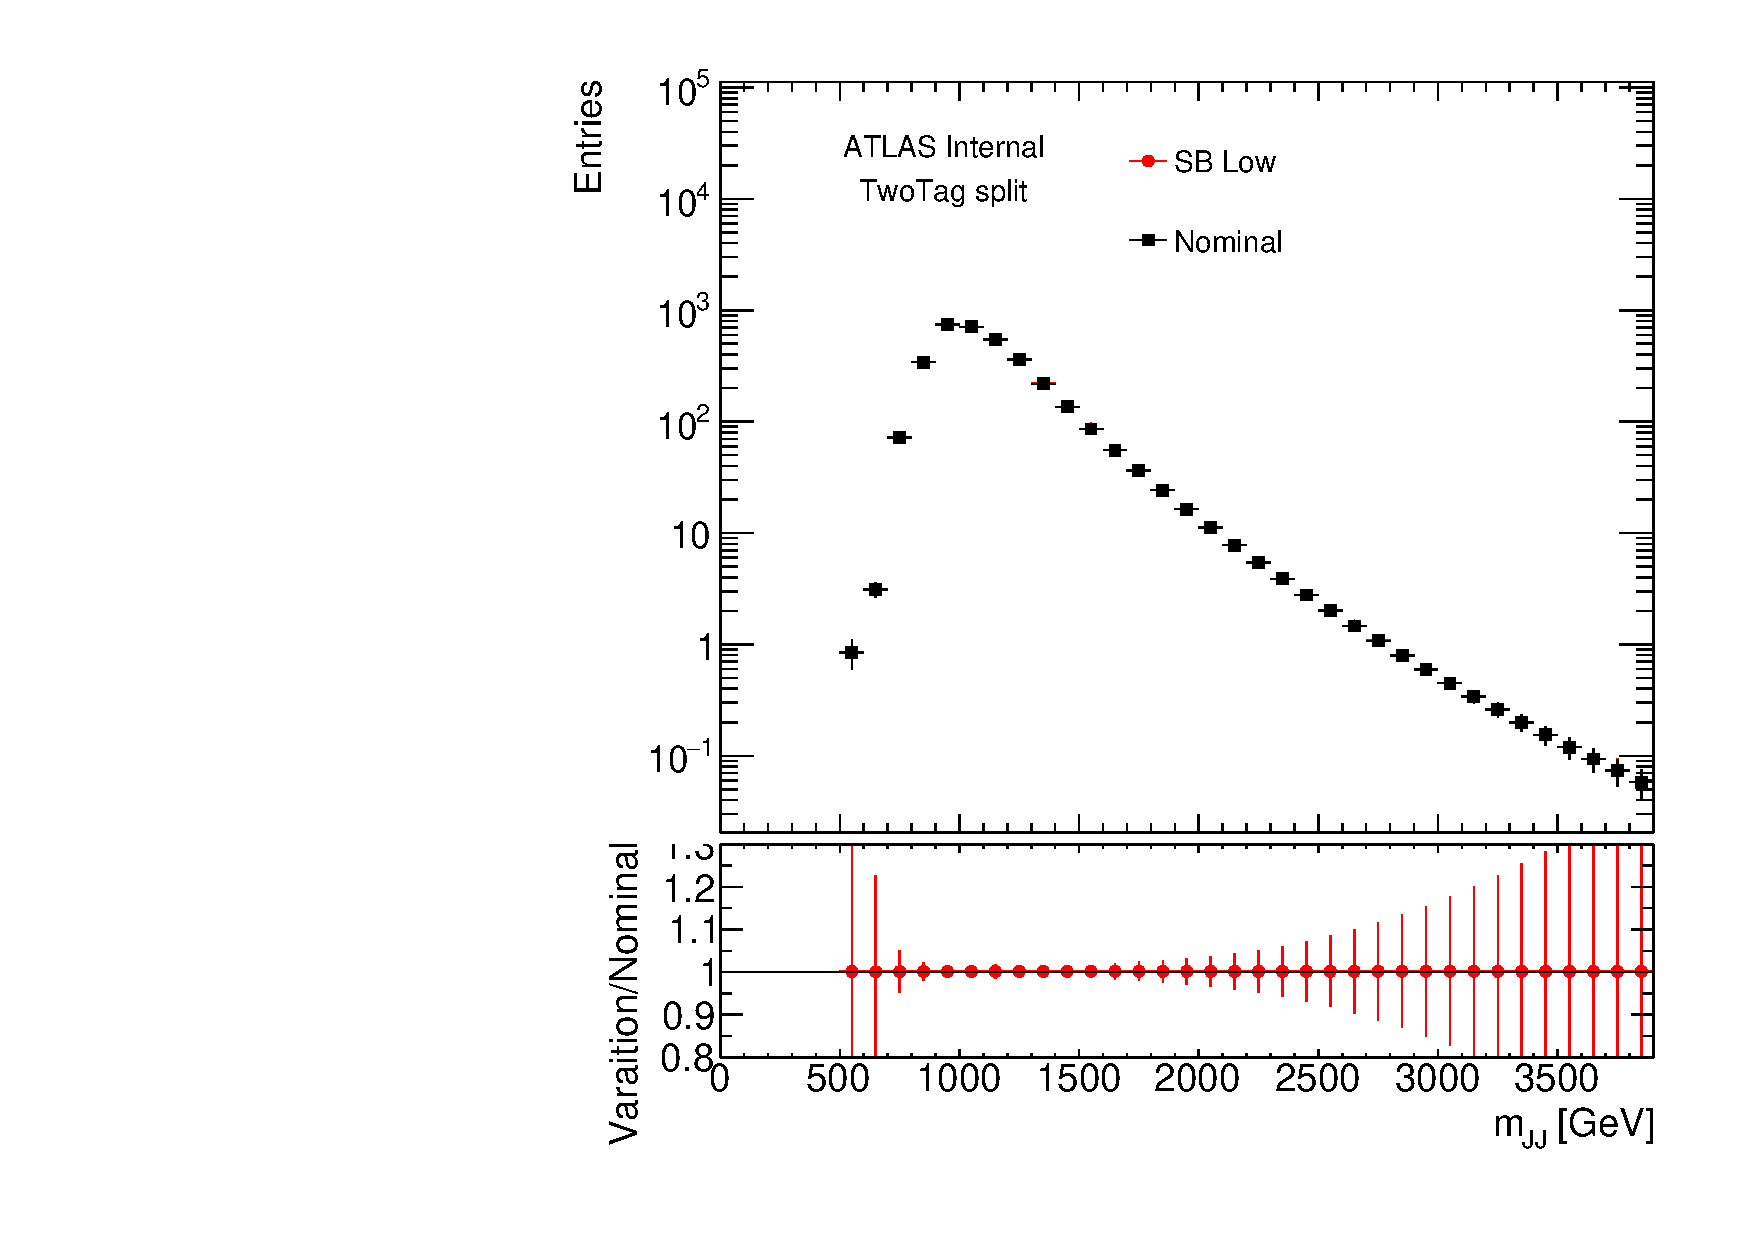
\includegraphics[width=0.25\textwidth,angle=-90]{figures/boosted/Syst_CRSB/SB_Low_compare_TwoTag_split_qcd_hh.pdf}
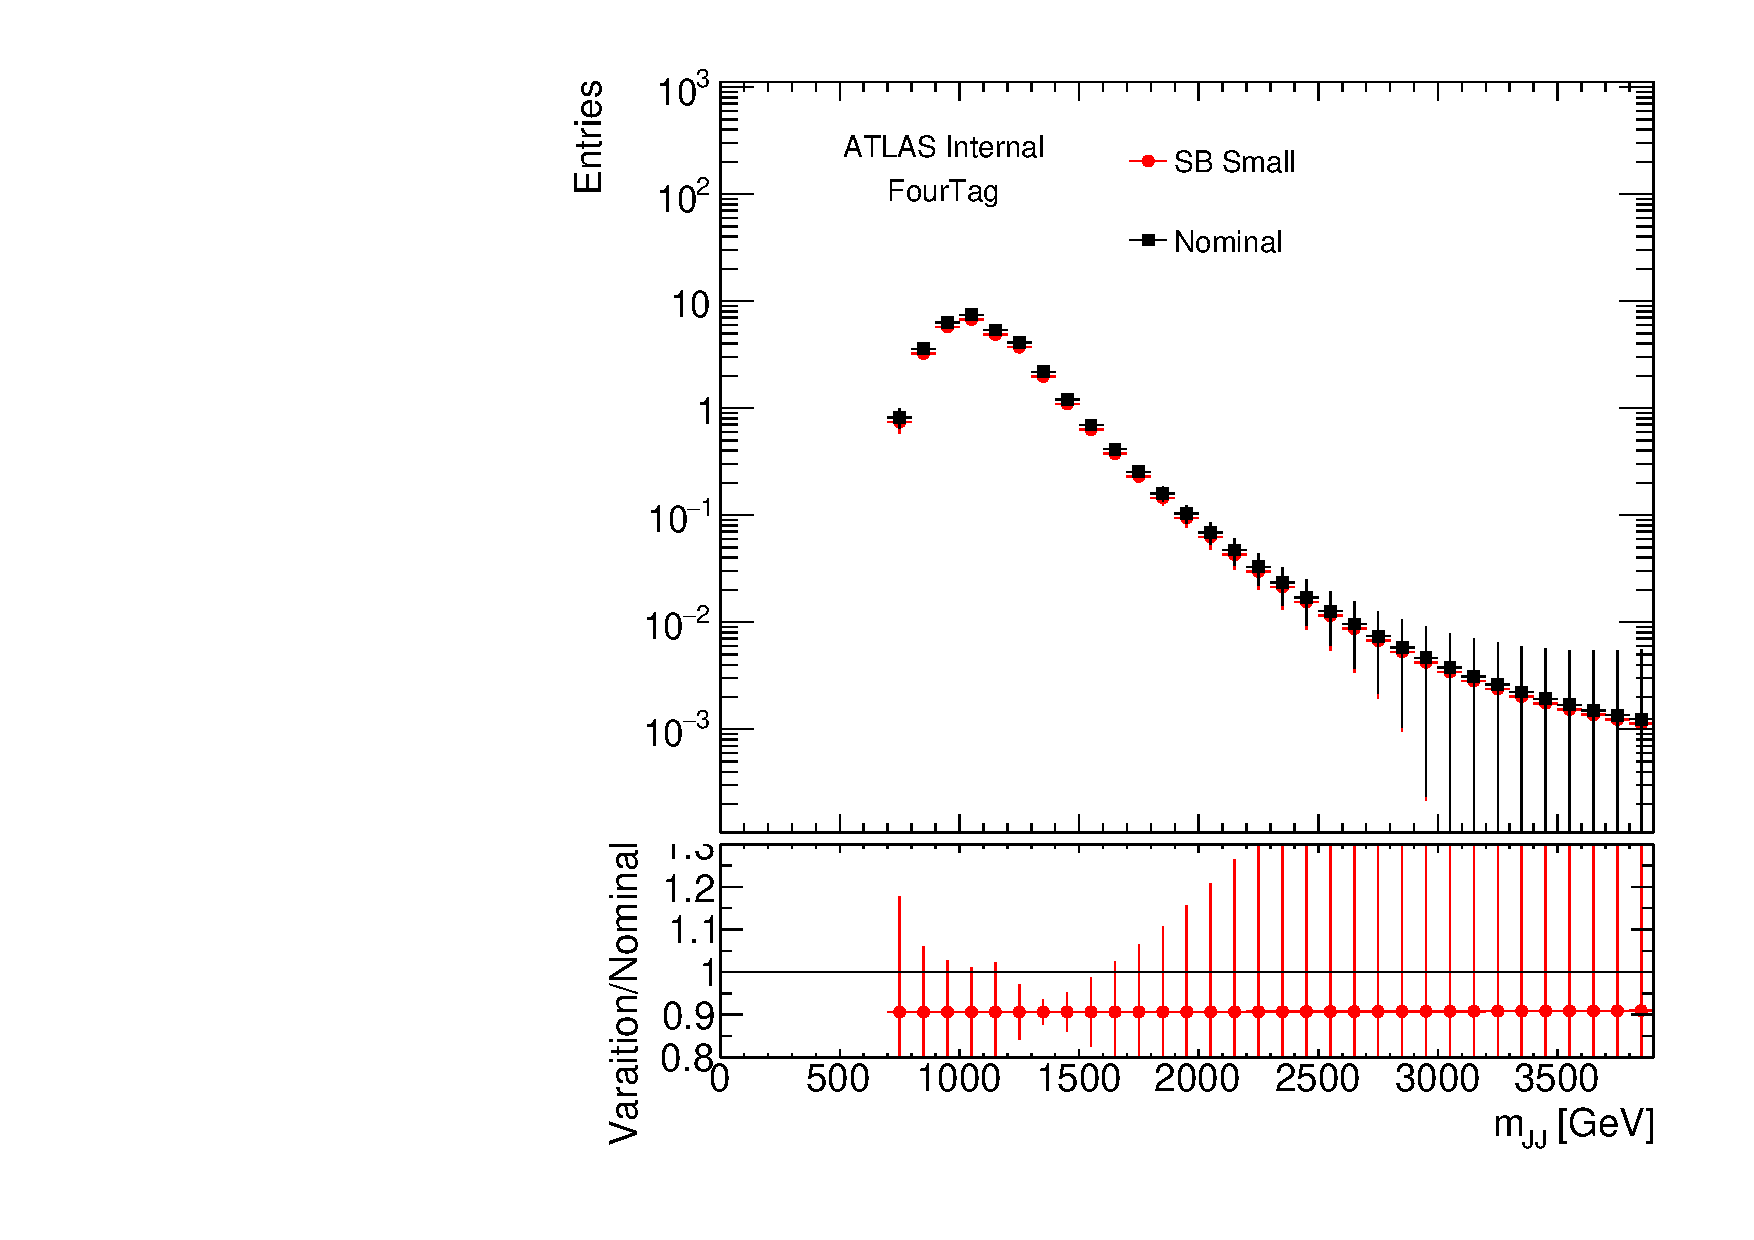
\includegraphics[width=0.25\textwidth,angle=-90]{figures/boosted/Syst_CRSB/SB_Small_compare_FourTag_qcd_hh.pdf}
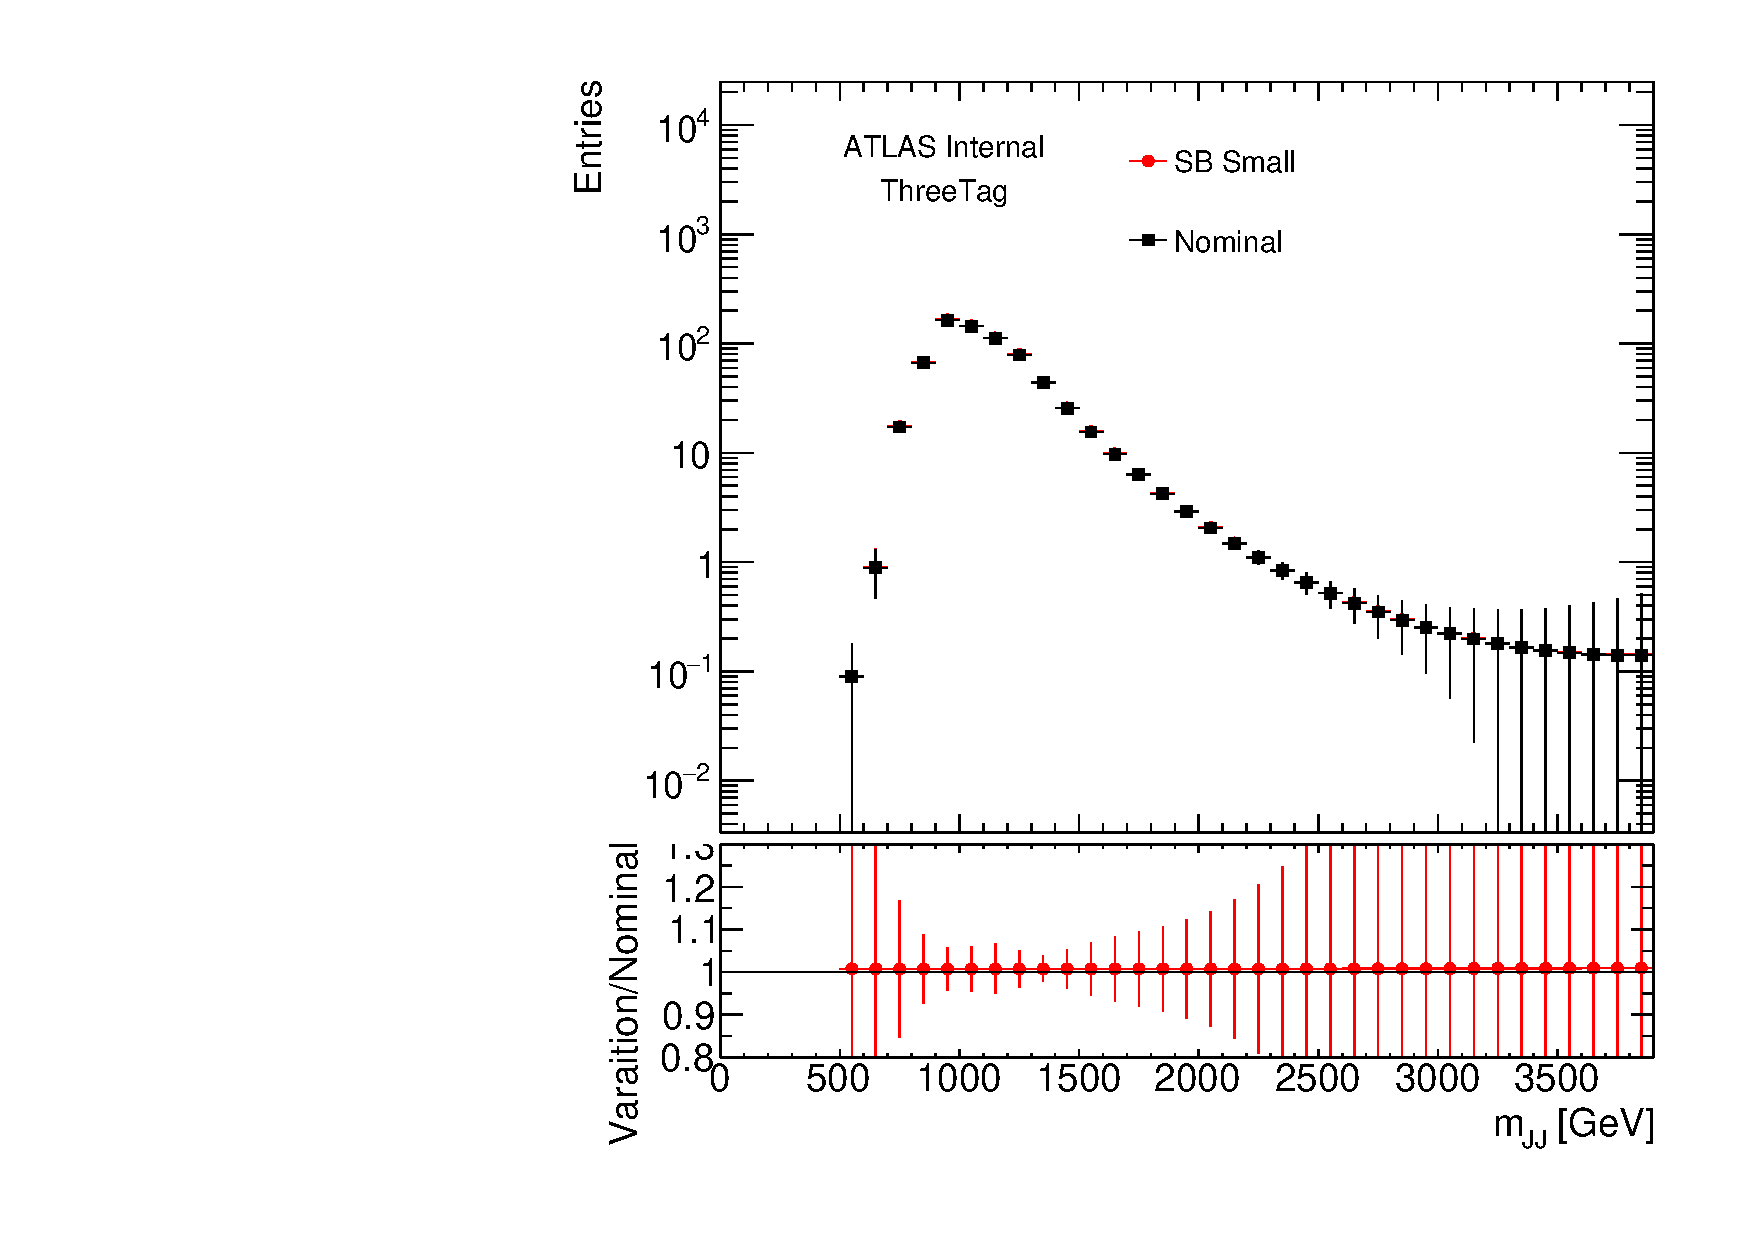
\includegraphics[width=0.25\textwidth,angle=-90]{figures/boosted/Syst_CRSB/SB_Small_compare_ThreeTag_qcd_hh.pdf}
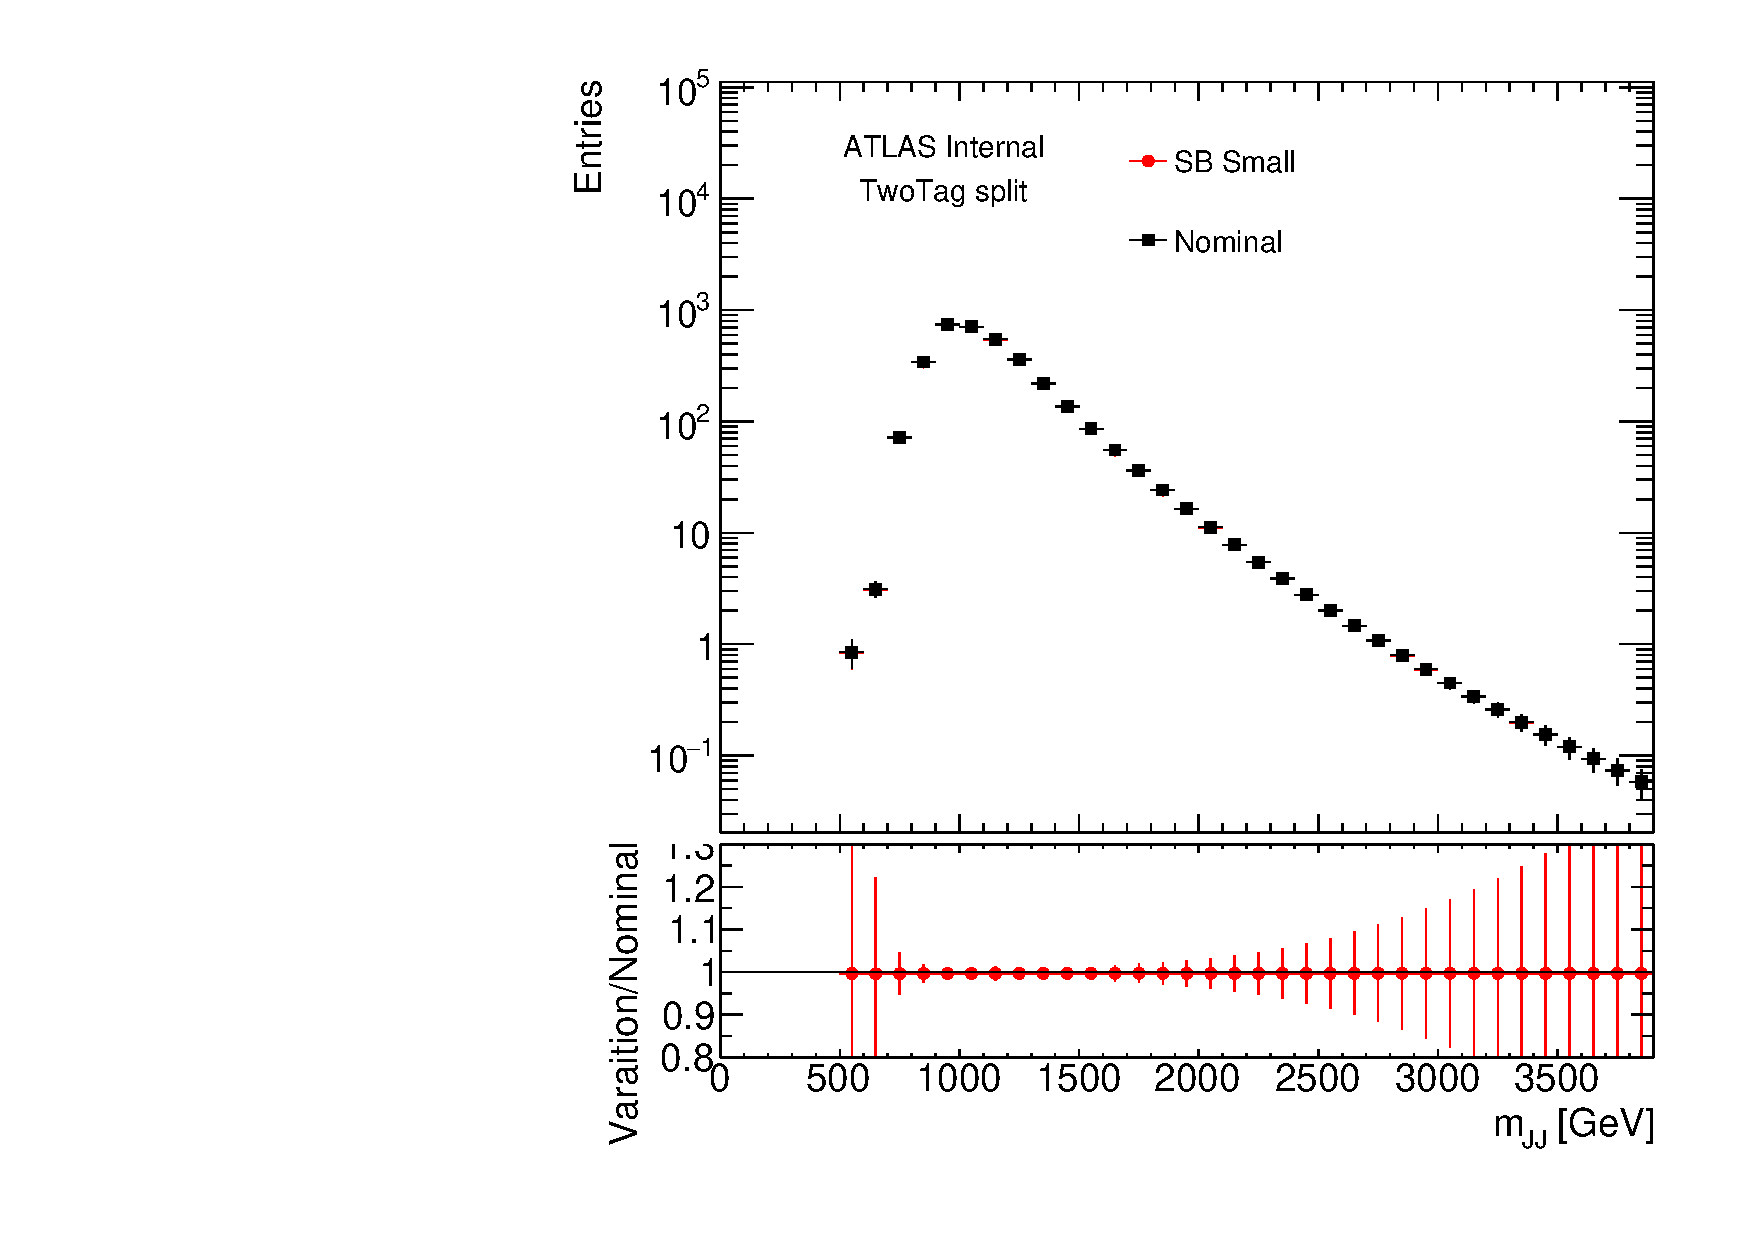
\includegraphics[width=0.25\textwidth,angle=-90]{figures/boosted/Syst_CRSB/SB_Small_compare_TwoTag_split_qcd_hh.pdf}
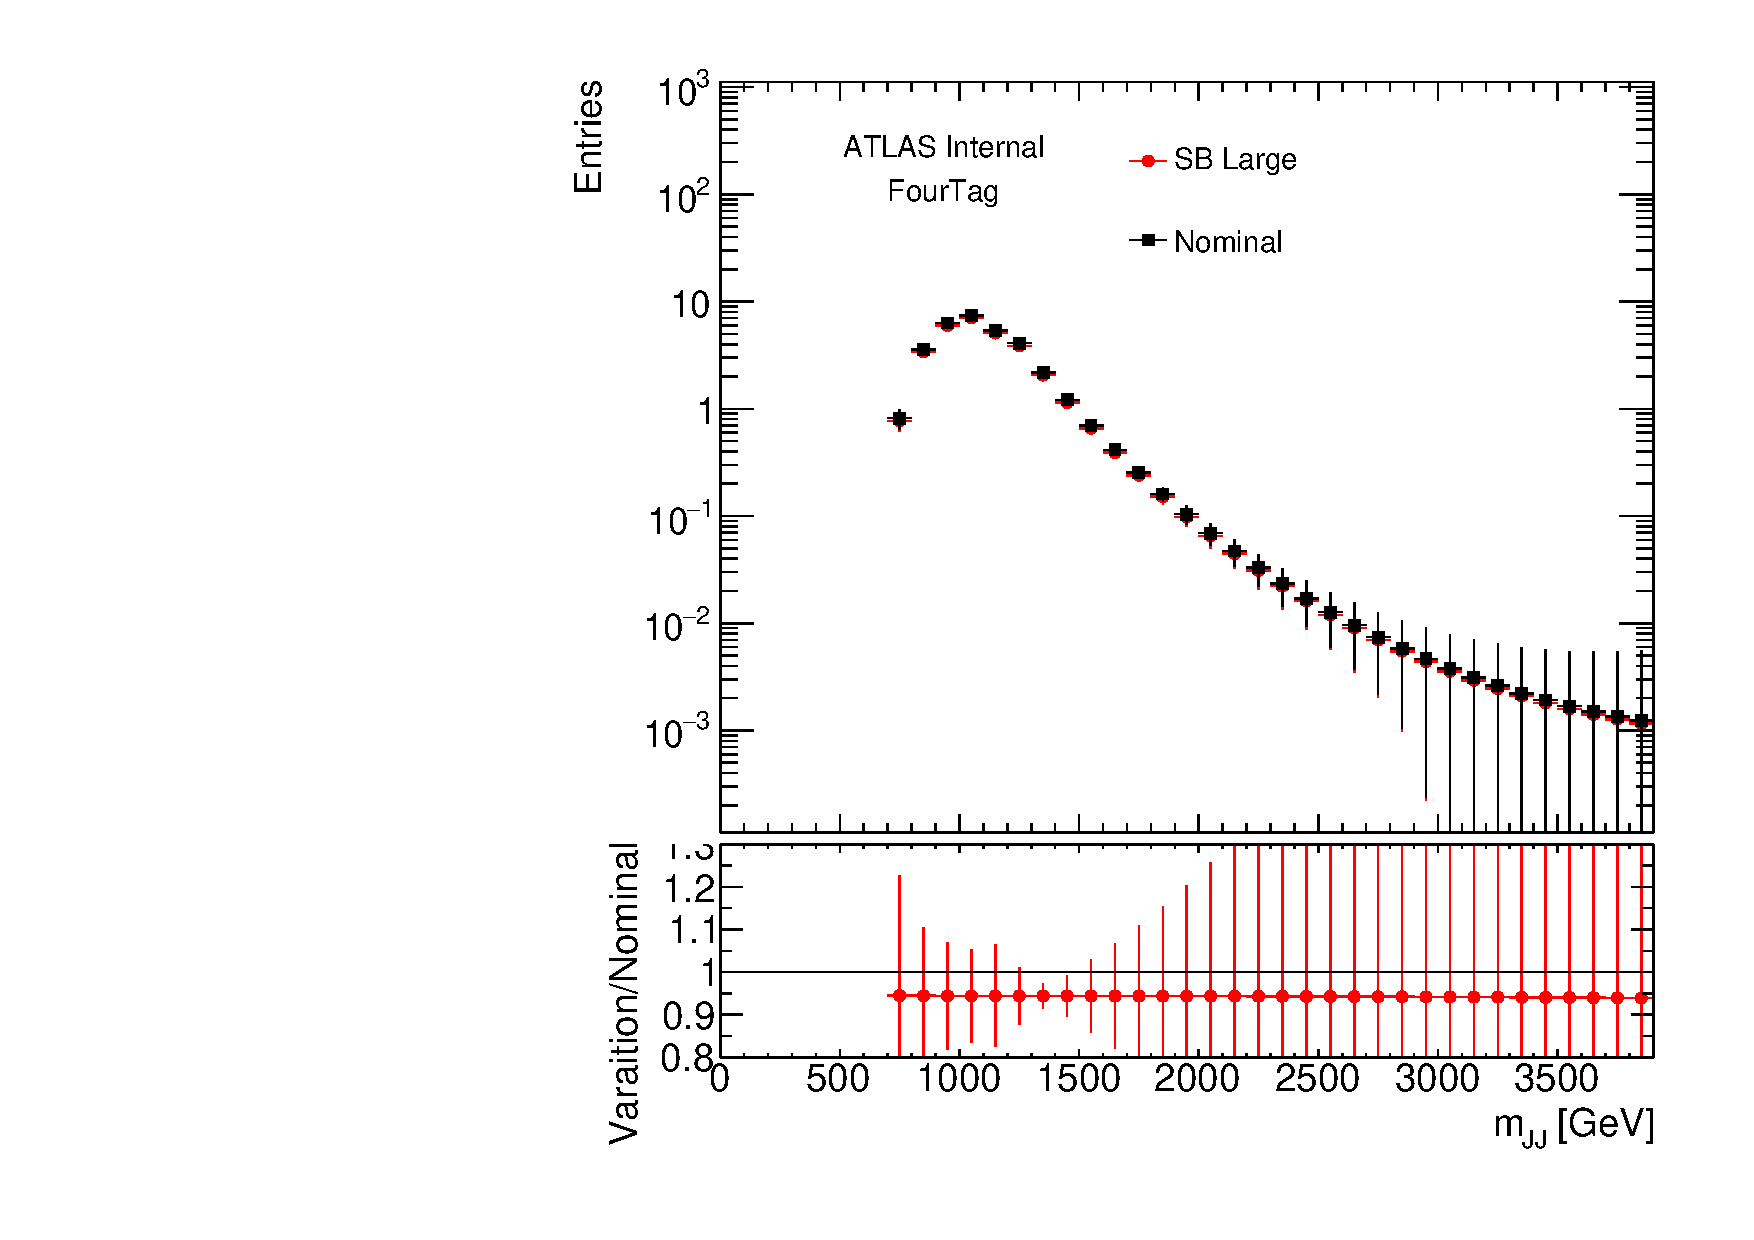
\includegraphics[width=0.25\textwidth,angle=-90]{figures/boosted/Syst_CRSB/SB_Large_compare_FourTag_qcd_hh.pdf}
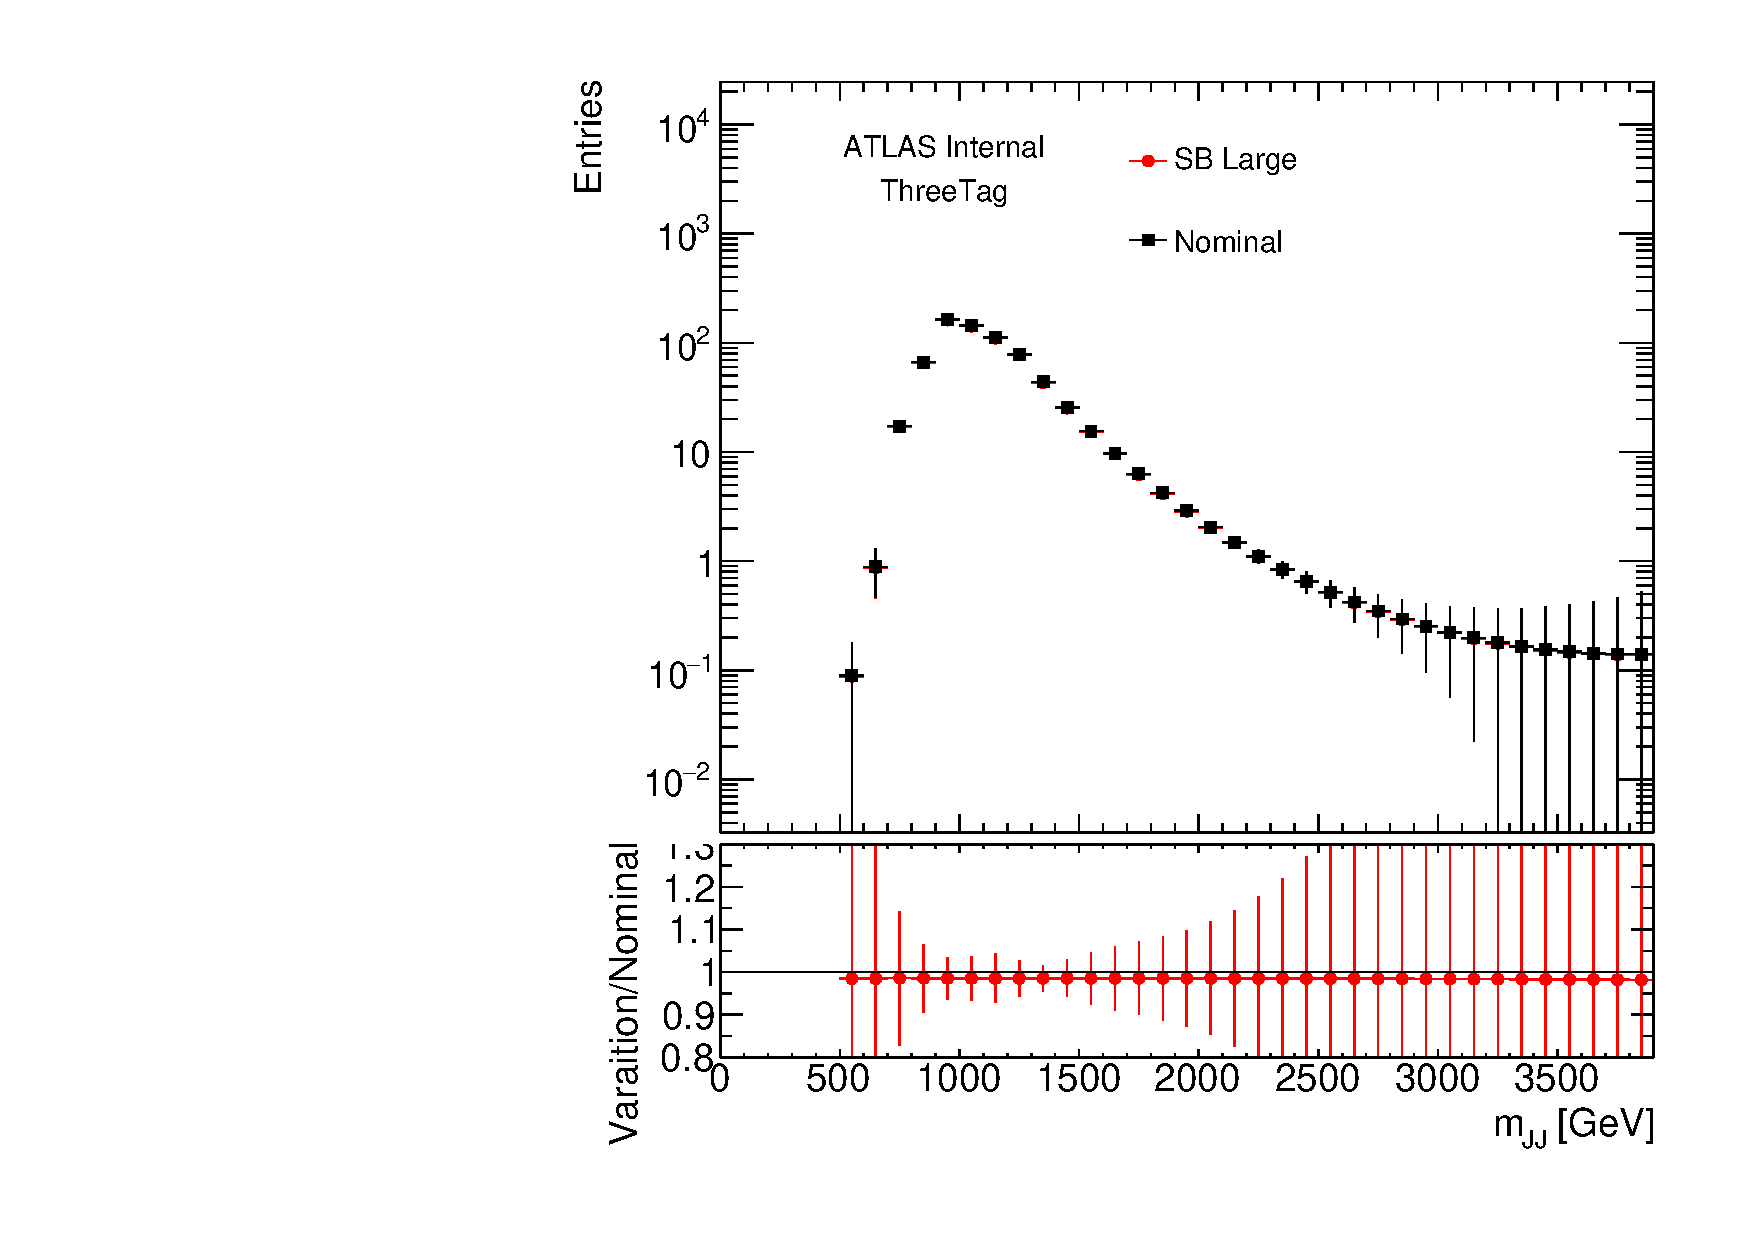
\includegraphics[width=0.25\textwidth,angle=-90]{figures/boosted/Syst_CRSB/SB_Large_compare_ThreeTag_qcd_hh.pdf}
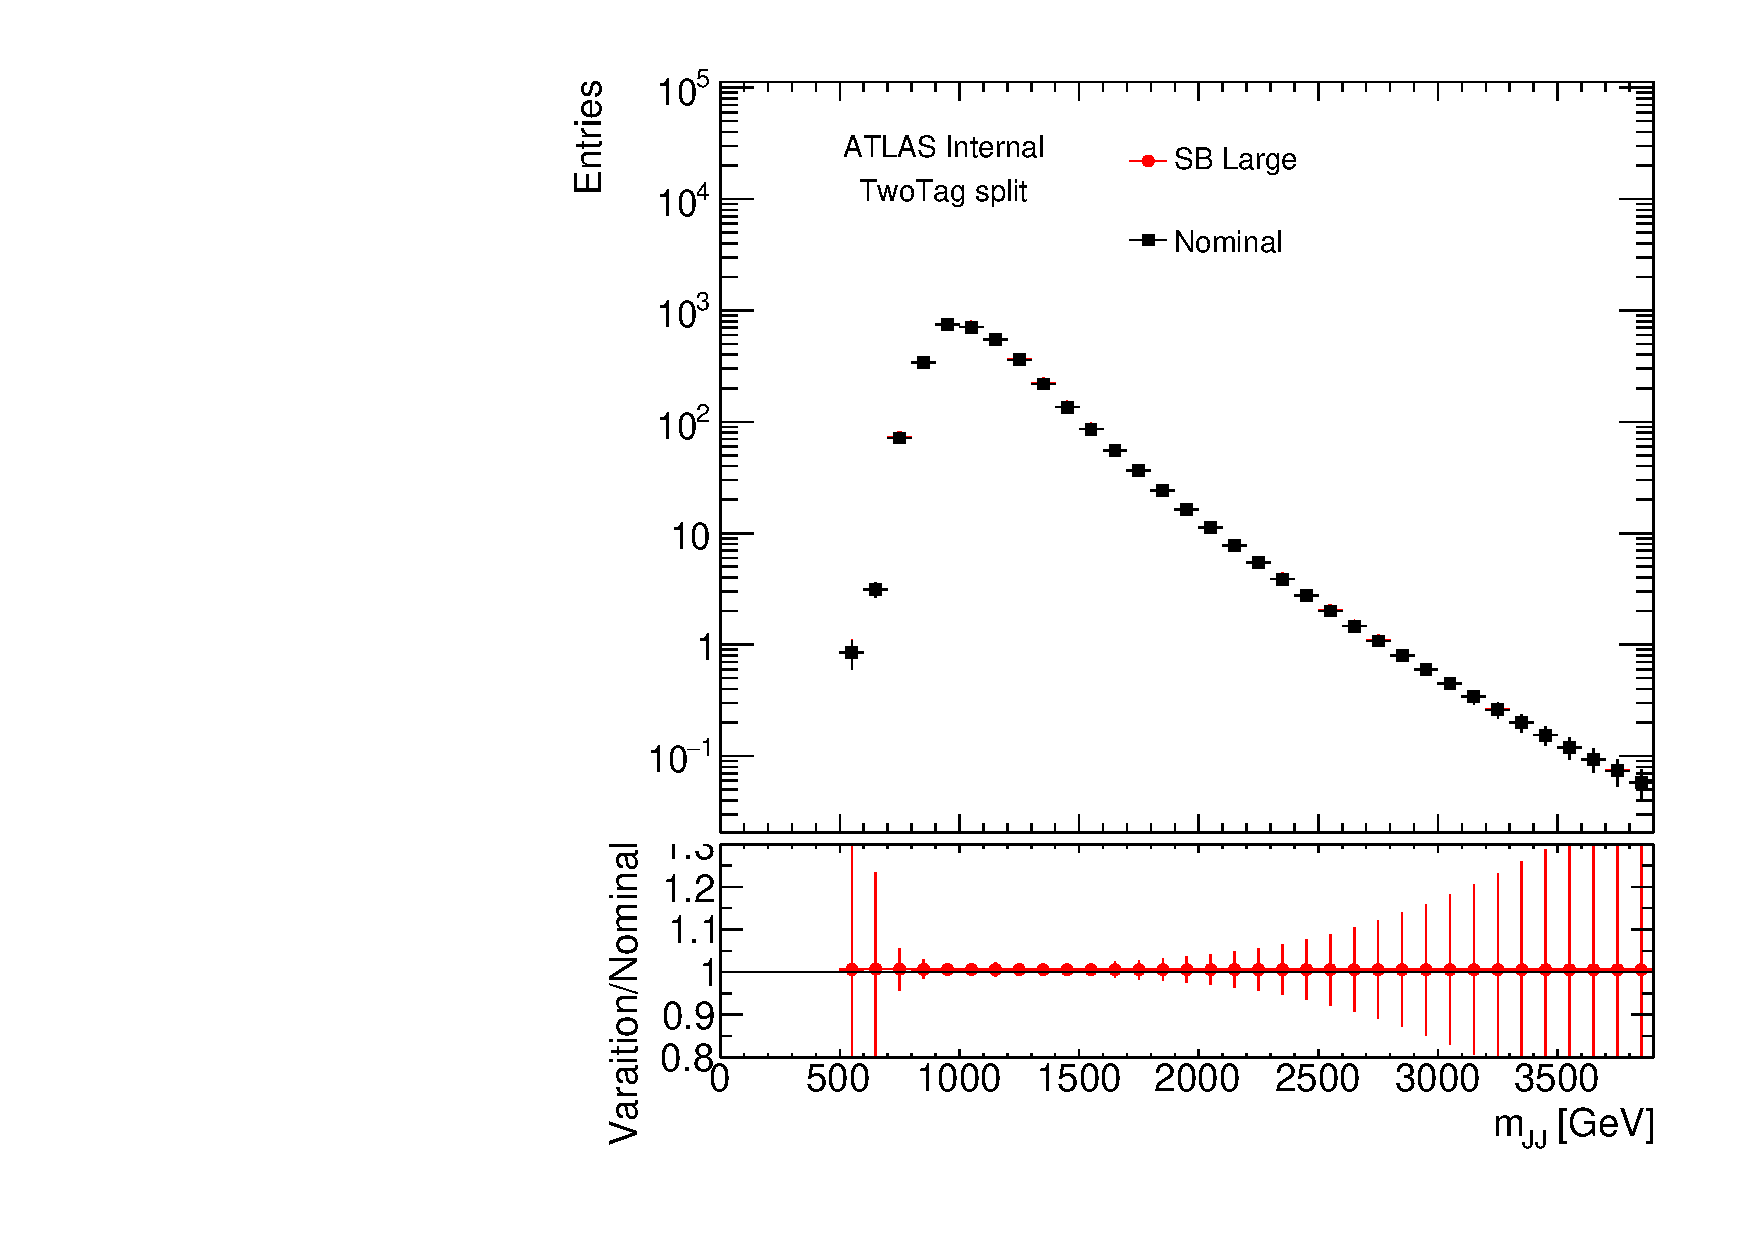
\includegraphics[width=0.25\textwidth,angle=-90]{figures/boosted/Syst_CRSB/SB_Large_compare_TwoTag_split_qcd_hh.pdf}
\end{center}
\caption{Comparisons of the nominal QCD shape prediction (black) with the results of control and sideband region variations (red). The ratio of the shape from each variation to the nominal shape is shown in the lower panel. The left column shows the relevant distributions for the $4b$ signal region, the middle column is for the $3b$ signal region, and the left column is for the $2bs$ signal region. The top row is for the high SB variation, the second row is for the low SB variation, the third row is for the small SB variation and the large raw is for the large SB variation.}
\label{CRSB:QCDShapeSR-SB}
\end{figure}
